 % vim: tw=80

\chapter[Measurement of the Triple-Differential Dijet Cross Section]{Measurement
of the Triple-Differential\\ Dijet Cross Section}
\label{sec:measurement}

The preceeding chapter laid the foundation for the triple-differential dijet
cross section measurement by presenting the NLO pQCD calculations and
demonstrating the observable's sensitivity to the PDFs. Especially the sizable
PDF uncertainties in phase space regions involving boosted dijet events indicate
that a sufficiently precise measurement could be exploited to better constrain
the PDFs. 

This chapter is dedicated to the measurement of the cross section from collision
data recorded by CMS during the 2012 LHC run at a center-of-mass energy of
\SI{8}{\TeV}. The first two sections give the definition of the measured cross
section and the analyzed data sets. Sec.~\ref{sec:event_selection} describes the
event selection in which clean dijet events are identified. Based on simulated
events, the detector response is studied and the jet energy resolution is derived
which is used subsequently to correct the measured cross section for detector
effects in an iterative unfolding procedure. A detailed study of all
experimental sources of uncertainty in Sec.~\ref{sec:experimental_uncertainties}
concludes the measurement.

Finally, the comparison of unfolded data to NLO predictions is presented in
Sec.~\ref{sec:nlo_comparisons}. Furthermore, comparisons to NLO calculations
complemented with matched parton showers, as made possible with the recently
released Herwig~7 MC event generator, are shown.
~\todo{mention powheg if ready}

\section{Cross Section Definition}

The observed dijet event yields are transformed into a triple-differential
cross section, which is defined as
%
\begin{equation*}
    \frac{d^3 \sigma}{d \ptavg d \ystar d \yboost} = \frac{1}{\epsilon
        \mathcal{L}_{\mathrm{int, eff}}} \frac{N}{\Delta \ptavg \Delta \ystar
        \Delta \yboost},
\end{equation*}
%
where $N$ denotes the number of dijet events, $\mathcal{L}_{\mathrm{int, eff}}$
the effective integrated luminosity and $\epsilon$ the product of trigger and
event selection efficiencies which are greater than 99\% in the measured phase
space. The cross section is normalized by the widths of the \ptavg, \ystar, and
\yboost bins. 

The size of the \ptavg bins is chosen based on the observed resolution for
\ptavg at the bin center. For simplification, the same bin widths are chosen
as for the inclusive jet cross section measurement, which has a slightly worse
resolution. The equidistant \ystar and \yboost bins start from zero and go up to
three with a bin size of one.

\section{Data samples}
\label{sec:data sets}

The measurement is based on data collected by CMS in the 2012 run
period of the LHC at a center-of-mass energy of \SI{8}{\TeV}. The accumulated
data corresponds to a total integrated luminosity of $\SI{19.71}{\fbinv}$. 

The 2012 LHC data taking is subdivided into four periods A, B, C and D and the
data sets are split accordingly into separate samples. Each data set is further
split into subsets containing only a fraction of all triggered events which are
grouped according to the physics purpose. This analysis relies on a range of jet
triggers. All events triggered by prescaled jet triggers were streamed into the
data sets \texttt{Jet} and \texttt{JetMon} while the events of unprescaled jet
triggers were moved into the data set \texttt{JetHT}. As this assignment changed
over the 2012 run periods, it was taken care to only select the correct subset
of events. Table~\ref{tab:data:data sets} presents the CMS collision data sets
analyzed in this thesis as well as the integrated luminosity collected in
each run period.

\begin{table}[htbp]
    \centering
    \caption[Datasets of the 2012 LHC run period]
       {The 2012 collision data of CMS comprises four data sets collected in the run periods
           A, B, C and D. The total integrated luminosity of all data collected
           in 2012 sums up to \SI{19.71}{\fbinv}.}
    \label{tab:data:data sets}
    \begin{tabular}{cccc}
    \toprule
    \textbf{run}  & \textbf{run range} & \textbf{data set}                       & \textbf{luminosity}\\
                  &                    &                                        & \si{\fbinv}\\\midrule
    A             & 190456--193621     & /Jet/Run2012A-22Jan2013-v1/AOD         & \num{0.88}\\
    B             & 193834--196531     & /Jet[Mon,HT]/Run2012B-22Jan2013-v1/AOD & \num{4.49}\\
    C             & 198022--203742     & /Jet[Mon,HT]/Run2012C-22Jan2013-v1/AOD & \num{7.06}\\
    D             & 203777--208686     & /Jet[Mon,HT]/Run2012D-22Jan2013-v1/AOD & \num{7.37}\\
    \bottomrule
    \end{tabular}
\end{table}
\todo{check for rounding errors}

\subsection{Monte Carlo Samples}

To compare the measured data with simulated events, two
Monte Carlo event generators were used, which are described in
Sec.~\ref{subsection:mc_generators}. Each MC generator is utilizing an optimized
tune to simulate the underlying event. Additionally, the Monte Carlo event samples
contain not only the hard scattering event, but also also an admixture
simulating the pileup collisions observed in real collisions.

The Madgraph Monte Carlo sample is generated with a multi-leg improved QCD
process. By using Madgraph, the LO matrix elements do not only contain the $2
\rightarrow 2$ matrix elements, but also multi-leg matrix elements. These better
describe multi-jet events, but have to be matched to the subsequent parton
shower. The underlying event is modeled using the tune Z2$^*$. The parton shower
and hadronization is carried out using the Pythia~6 event generator interfaced
to Madgraph by the LHE event record~\cite{Alwall:2006yp}. This simulated events
sample is the main sample used for data comparisons, not because of the
multileg-improved matrix elements which are not as important for the dijet
analysis in this thesis, but because of the huge number of events generated and simulated.

Furthermore, a data sample generated with Pythia~8 is used. While including only the $2
\rightarrow 2$ LO matrix elements, the event simulation and the underlying event
tune are improved in this newer version of the Pythia Monte Carlo generator.

To be able to perform comparisons between data and simulated events on
reconstructed level, events from both MC event generators were propagated
through the complete simulation of the CMS detector. This allows for further
studies like the measurement of the jet transverse momentum resolution which are
needed to finally correct the measured cross sections for detector effects.

Predictions of jet cross sections, especially those involving the jet transverse
momenta, are notoriously difficult to be calculated because of the steeply
falling spectrum. Consequently, it is not possible to generate enough events to
populate all the phase space up to highest \pt with a sufficiently large
number of events. However, there are two approaches to overcome this issue.
The first method involves the reweighting of the generation process to generate
more events at high transverse momentum. Unfortunately, this spoils the absolute
normalization of the cross section as well as it involves the consideration of
huge event weights. The second method is based on splitting the phase space in
multiple regions, in which events are generated separately. The different phase
space regions are then stitched together later in the data analysis while taking
into account the cross sections in the different phase space regions. 

The Madgraph sample is split into four regions according to the scalar sum of
the transverse momenta, $H_{\mathrm{T}}$, while the Pythia 8 sample is split
into twelve data sets according to the transverse momentum of the leading jet.
Table~\ref{tab:mc_samples} shows all Monte Carlo data sets as well as the cross
section and the generated number of events.

\section{Event selection}
\label{sec:event_selection}

The selection of events is based on several quality criteria which are either
recommended by CMS or developed specifically for this analysis to yield clean
dijet events.  Furthermore, phase space cuts on the jets ensure the
applicability and comparability of NLO theory calculations.

\subsection{Certified Data Selection}

The first step in the event processing chain is to only pick data from runs and
luminosity sections which fulfill certain criteria. These criteria include
proper performance of all detector subsystems as well as the passing of data
quality monitoring (DQM) steps during the validation process. The good
lumisections within a run are announced using a JSON data file, called
\textsc{Golden JSON}. The applied lumisection certification
file\footnote{\texttt{Cert\_190456-208686\_8TeV\_22Jan2013ReReco\_Collisions12\_JSON}}
in this analysis is based on the final event reconstruction of the 2012 CMS data
sets.

\subsection{Trigger Selection}

To measure and reconstruct the \ptavg spectrum of dijet production, a set of
single jet triggers has been used. Single jet triggers consist of one L1 trigger
seed and multiple HLT filters. The L1 trigger has a lower threshold to ensure
full efficiency versus \pt of the HLT trigger. Since the \pt spectrum is steeply
falling and the rates for low-\pt jets are very high, it is not feasible to use
a single unprescaled trigger for the selection of all interesting events.
Instead, a set of five prescaled low-\pt trigger paths, each with different
prescale value, is used to collect sufficient data in the lower part of the \pt
spectrum.  Additionally, one unprescaled trigger is used in the high \pt region, in
which the rate is sufficiently small to collect and store all
events. A prescale value of $n$ means, that only every $n$-th event accepted by
a trigger, is kept. Of course, the applied prescale values have to be taken into
account when the original spectrum is reconstructed. 

\begin{table}[htbp]
    \centering
    \caption[Single Jet Trigger Paths]{List of all single jet trigger paths used in the analysis. Each
        trigger is employed in a mutually exclusive phase space region in \ptavg in which
        the trigger exhibits an efficiency larger than 99\%. The column
        $p_{\mathrm{T},99\%}$ indicates the value at which each trigger reaches
        that value. The last column reports the effective luminosity seen by
        each trigger. This number, divided by the total integrated luminosity of
        \SI{19.71}{\fbinv}, gives the effective prescale applied on a trigger
        over the whole run period.}
    \label{tab:triggers}
    \begin{tabular}{lcccc}
        \toprule
        \textbf{Trigger path}        & \textbf{L1 threshold} & \textbf{HLT threshold} & \boldmath$p_{\mathrm{T},99\%}$ & \textbf{Eff. Lumi} \\
                                     & \si{\GeV}             & \si{\GeV}              & \si{\GeV}              & \si{\fbinv}\\\midrule
                      HLT\_PFJet40   & 16                    & 40                     & --                     & \num{0.8e-4}\\
                      HLT\_PFJet80   & 36                    & 80                     & 123                    & \num{0.21e-2}\\
                      HLT\_PFJet140  & 68                    & 140                    & 192                    & \num{0.56e-1}\\
                      HLT\_PFJet200  & 92                    & 200                    & 263                    & \num{0.26}\\
                      HLT\_PFJet260  & 128                   & 260                    & 353                    & \num{1.06}\\
                      HLT\_PFJet320  & 128                   & 320                    & 412                    & \num{19.71}\\
        \bottomrule
    \end{tabular}
\end{table}

Table~\ref{tab:triggers} shows all single jet triggers used in the data
analysis. Each trigger is used in mutually exclusive regions of \ptavg, in which
the trigger is fully efficient.

\begin{figure}[htbp]
    \centering
    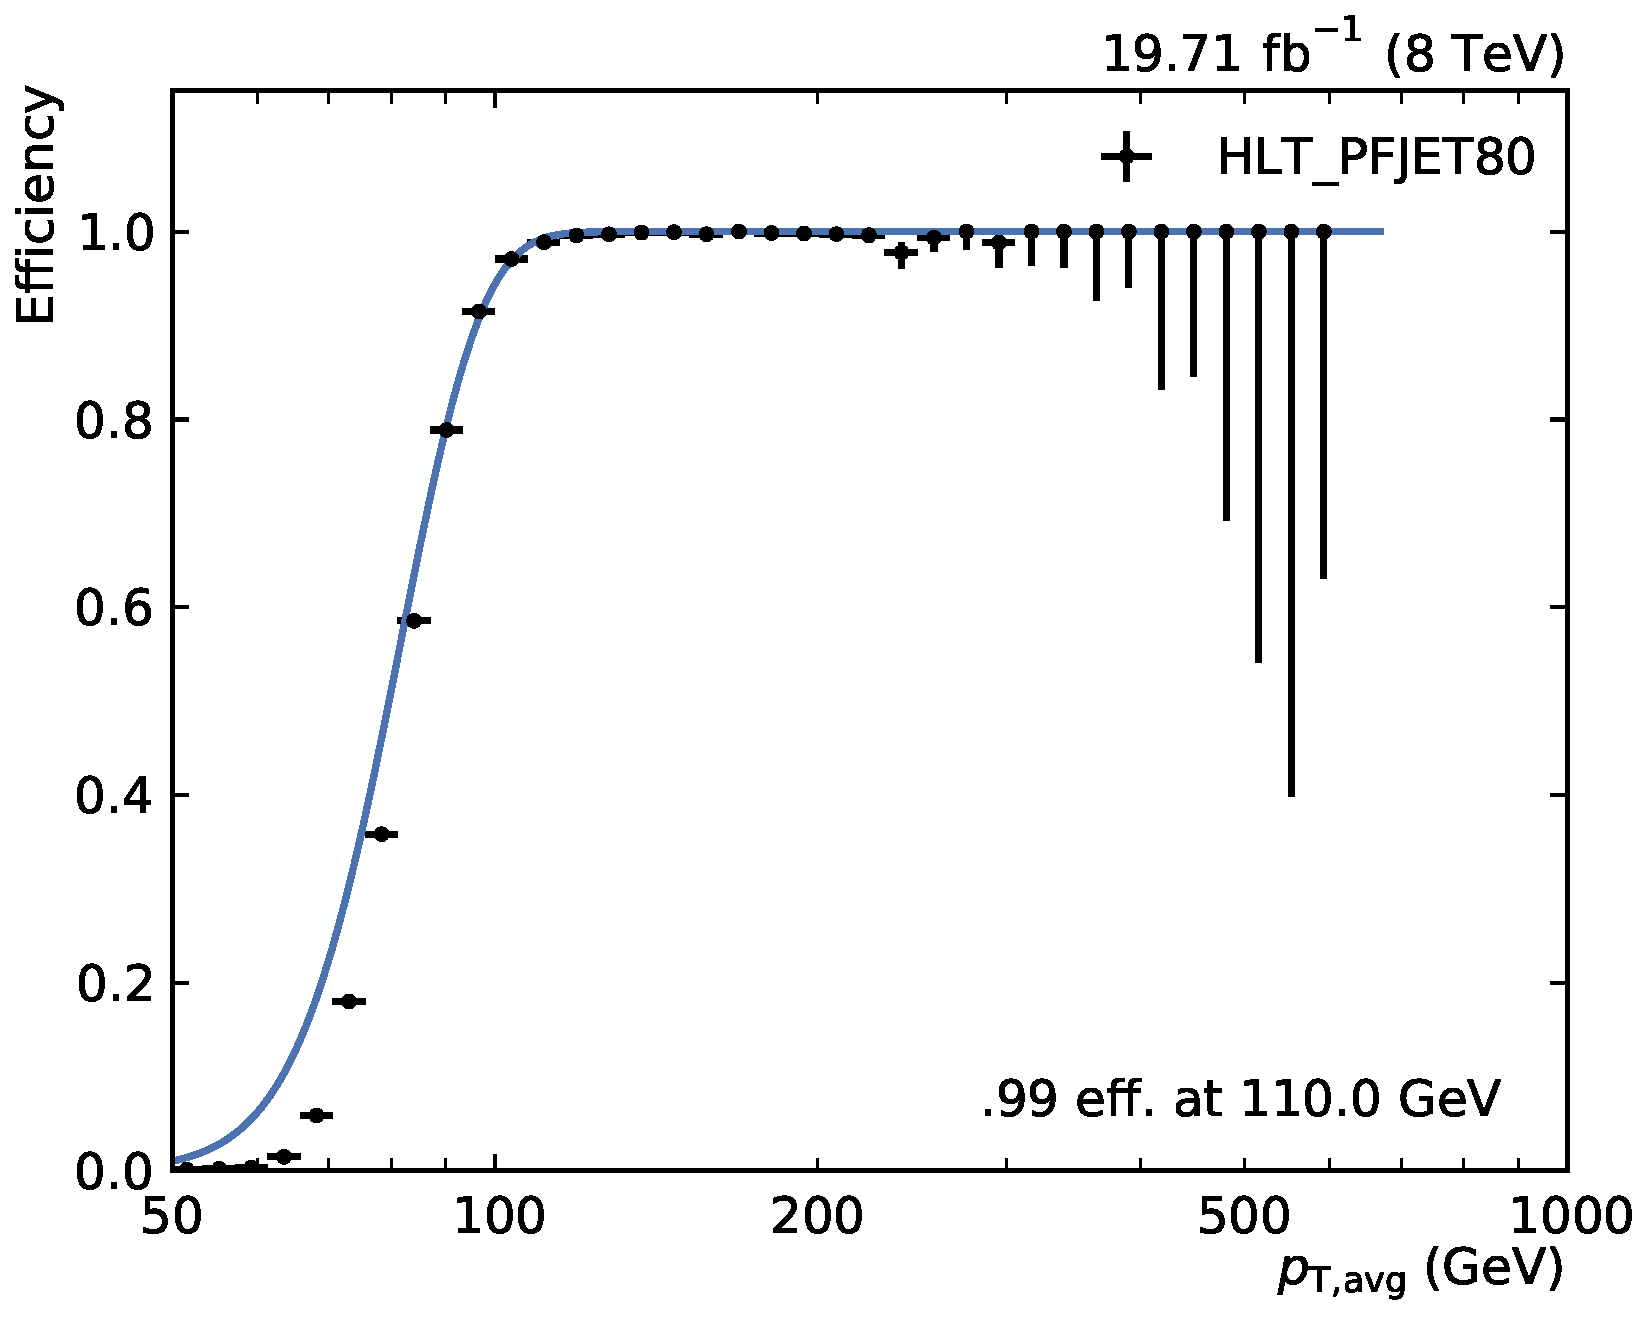
\includegraphics[width=0.49\textwidth]{figures/measurement/trigger_eff_HLT_PFJET80_default.pdf}\hfill
    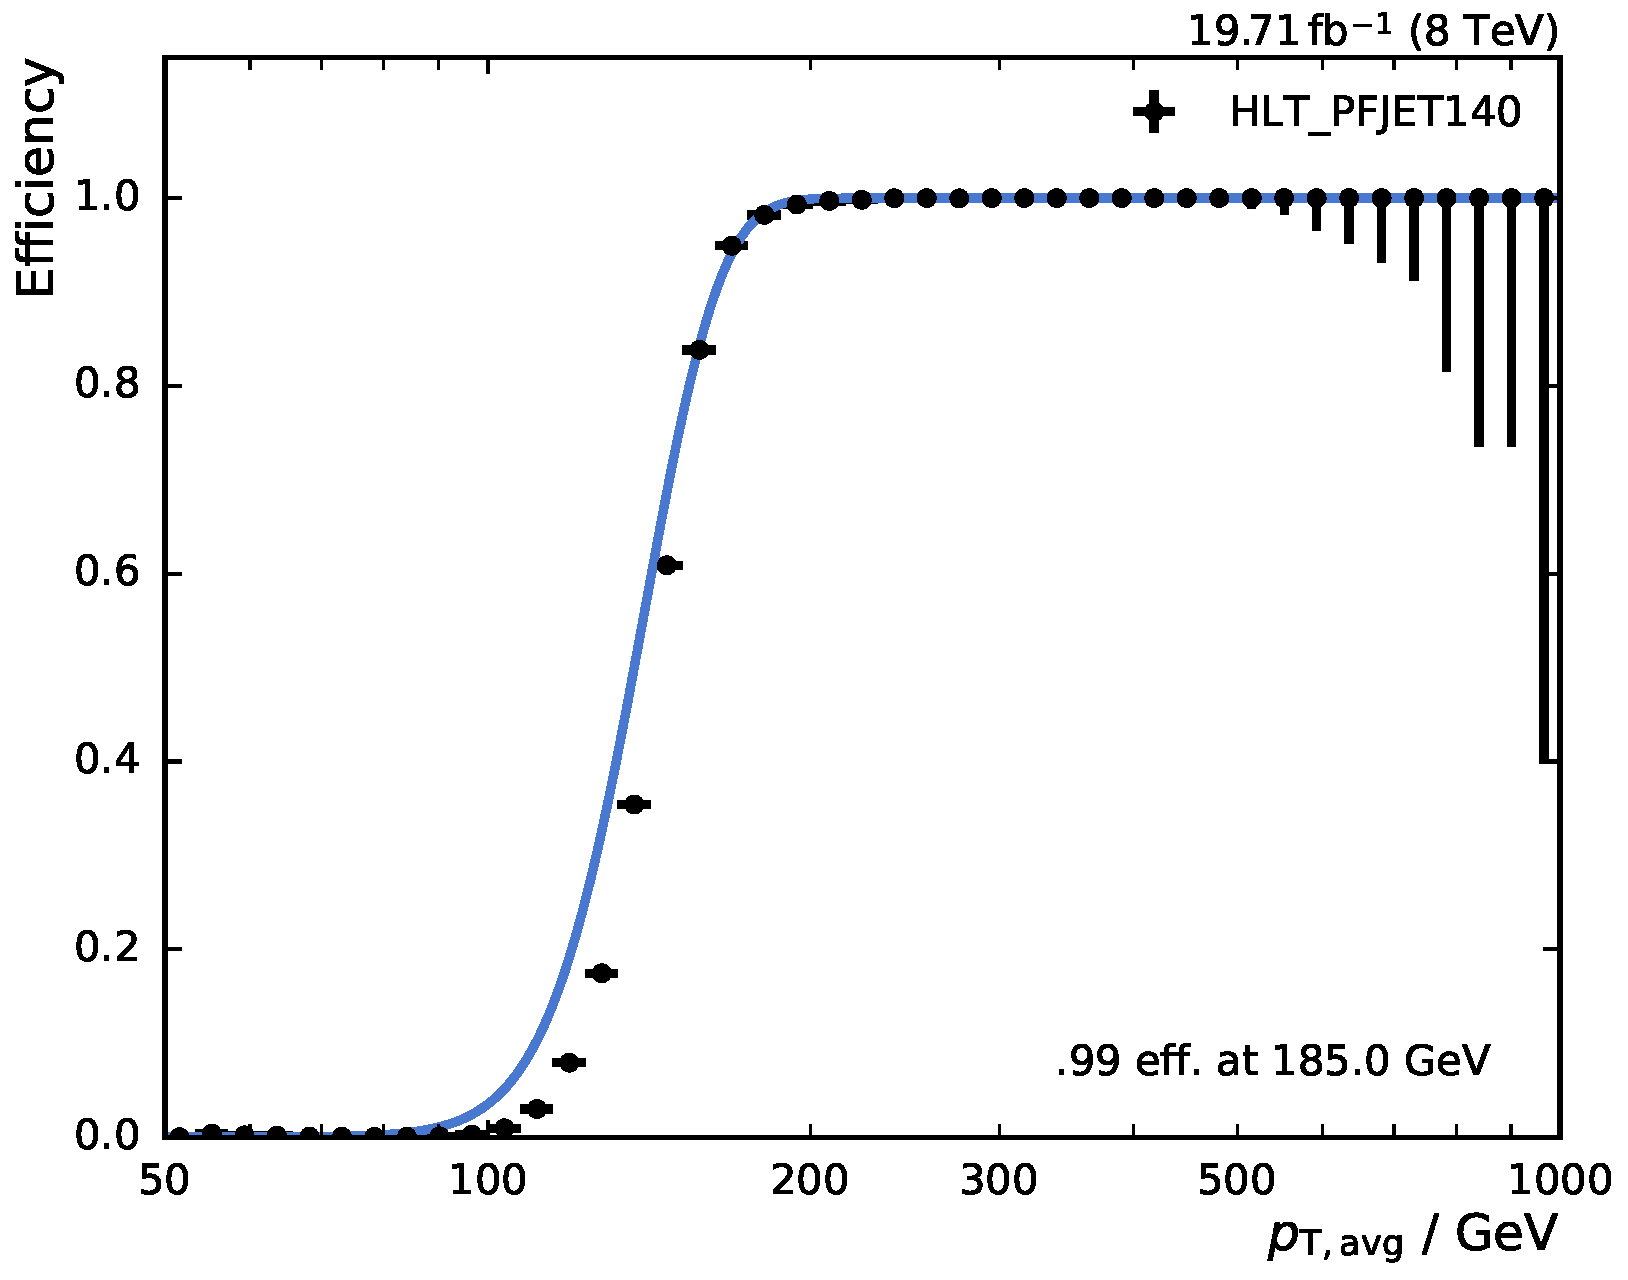
\includegraphics[width=0.49\textwidth]{figures/measurement/trigger_eff_HLT_PFJET140_default.pdf}
    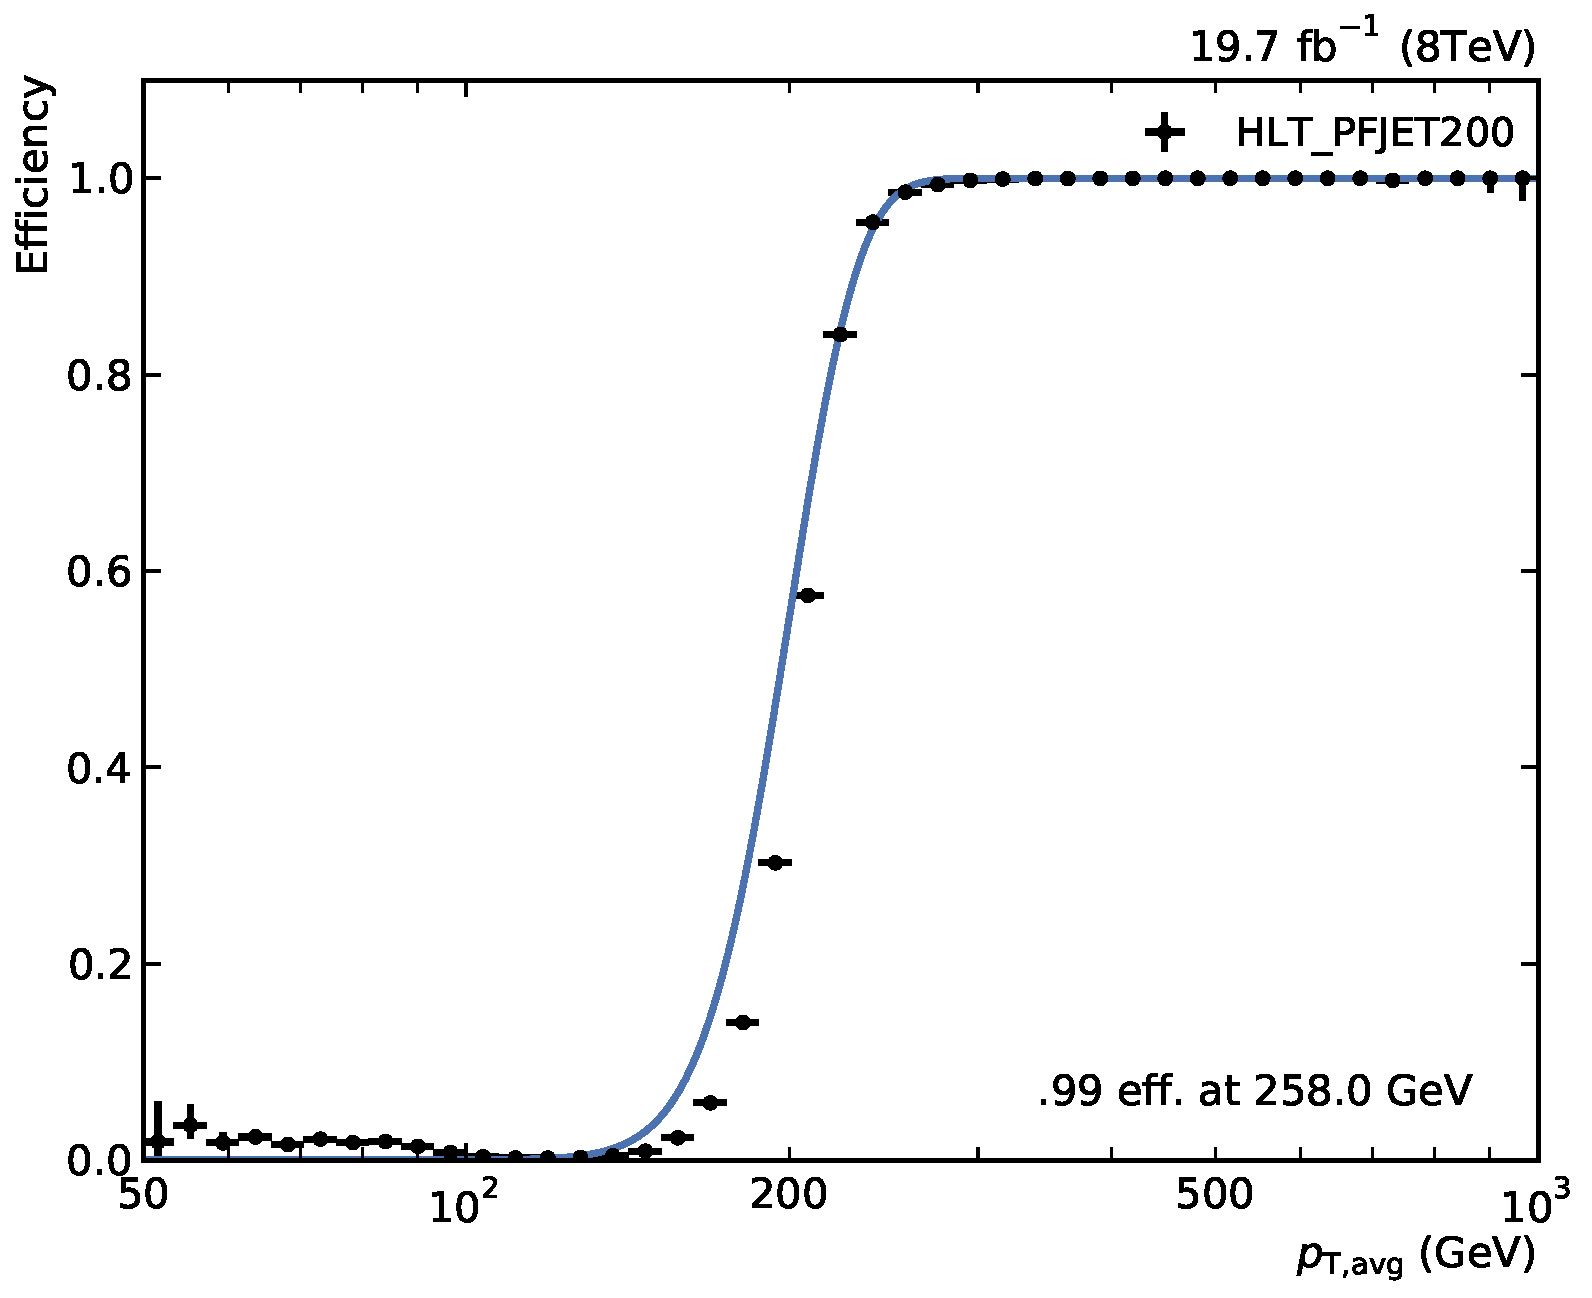
\includegraphics[width=0.49\textwidth]{figures/measurement/trigger_eff_HLT_PFJET200_default.pdf}\hfill
    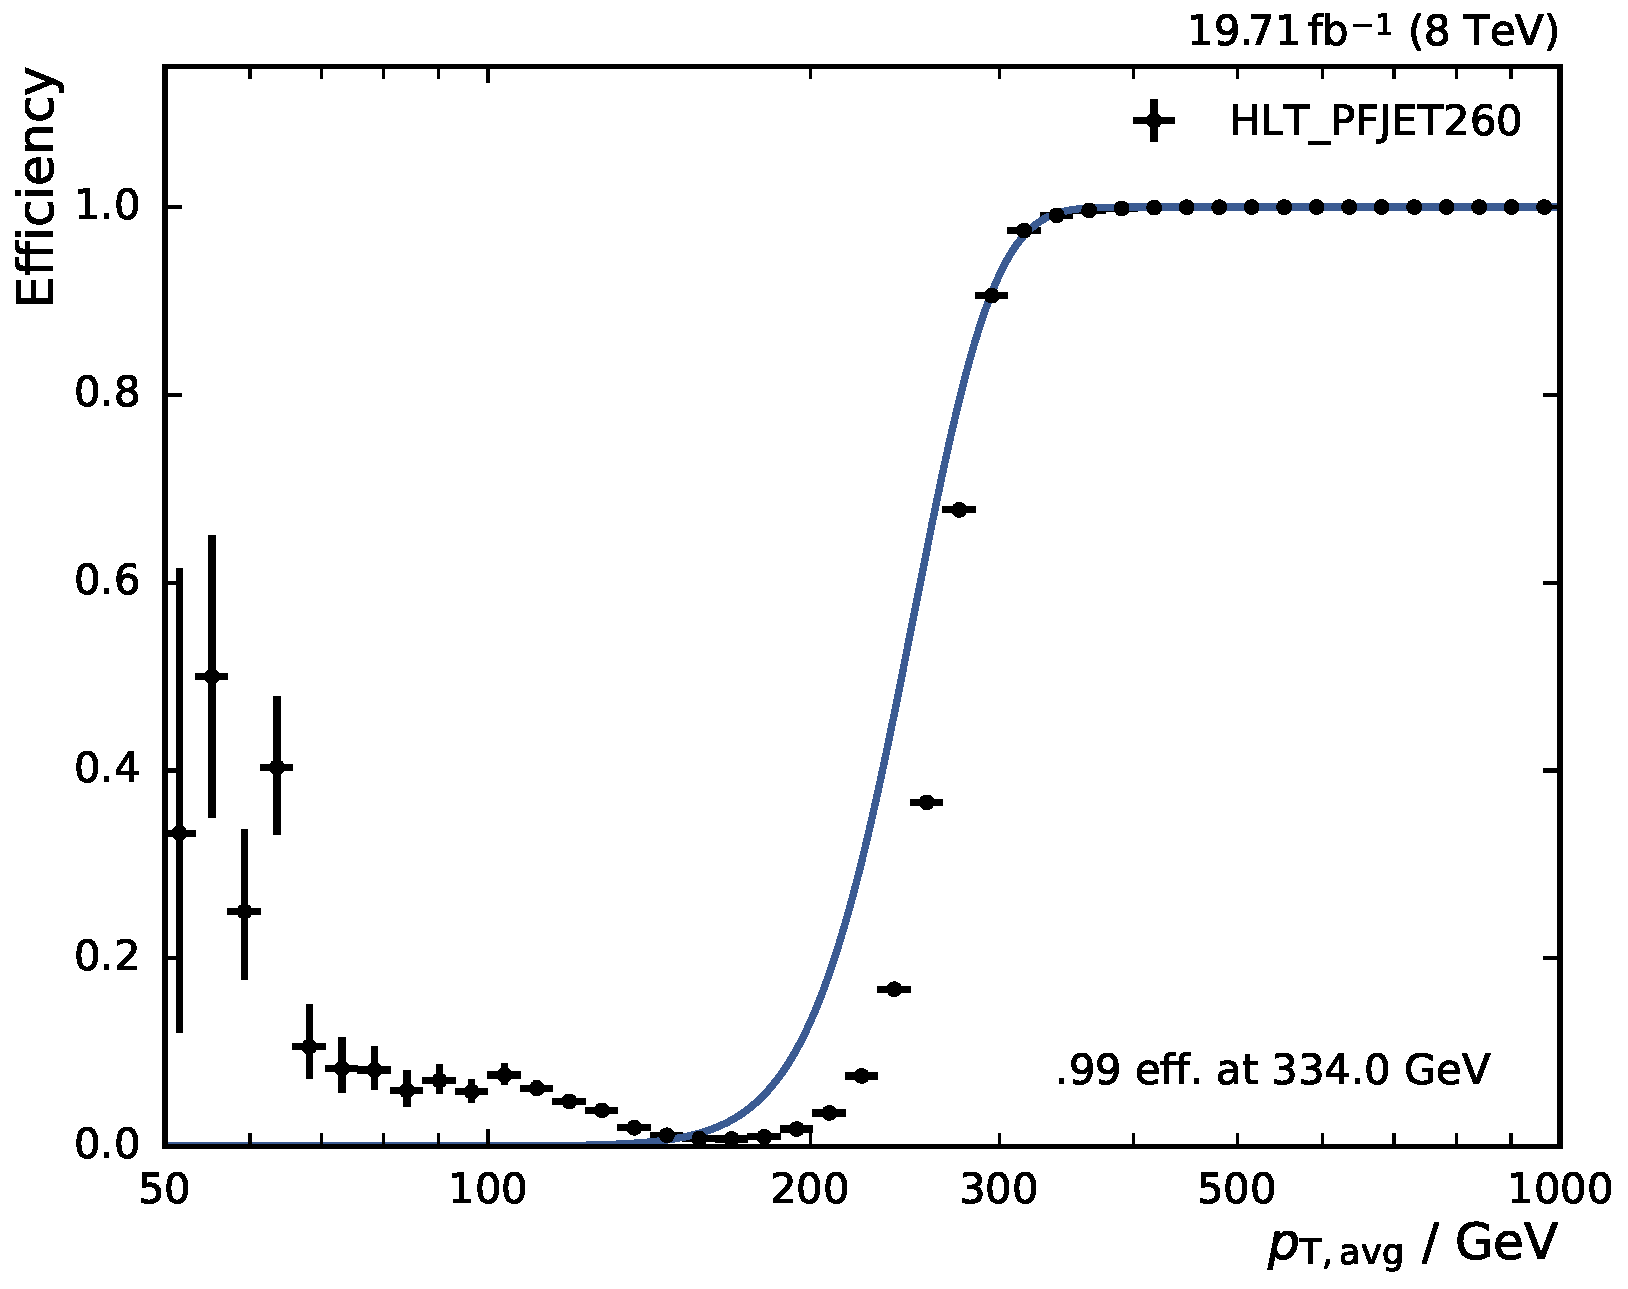
\includegraphics[width=0.49\textwidth]{figures/measurement/trigger_eff_HLT_PFJET260_default.pdf}
    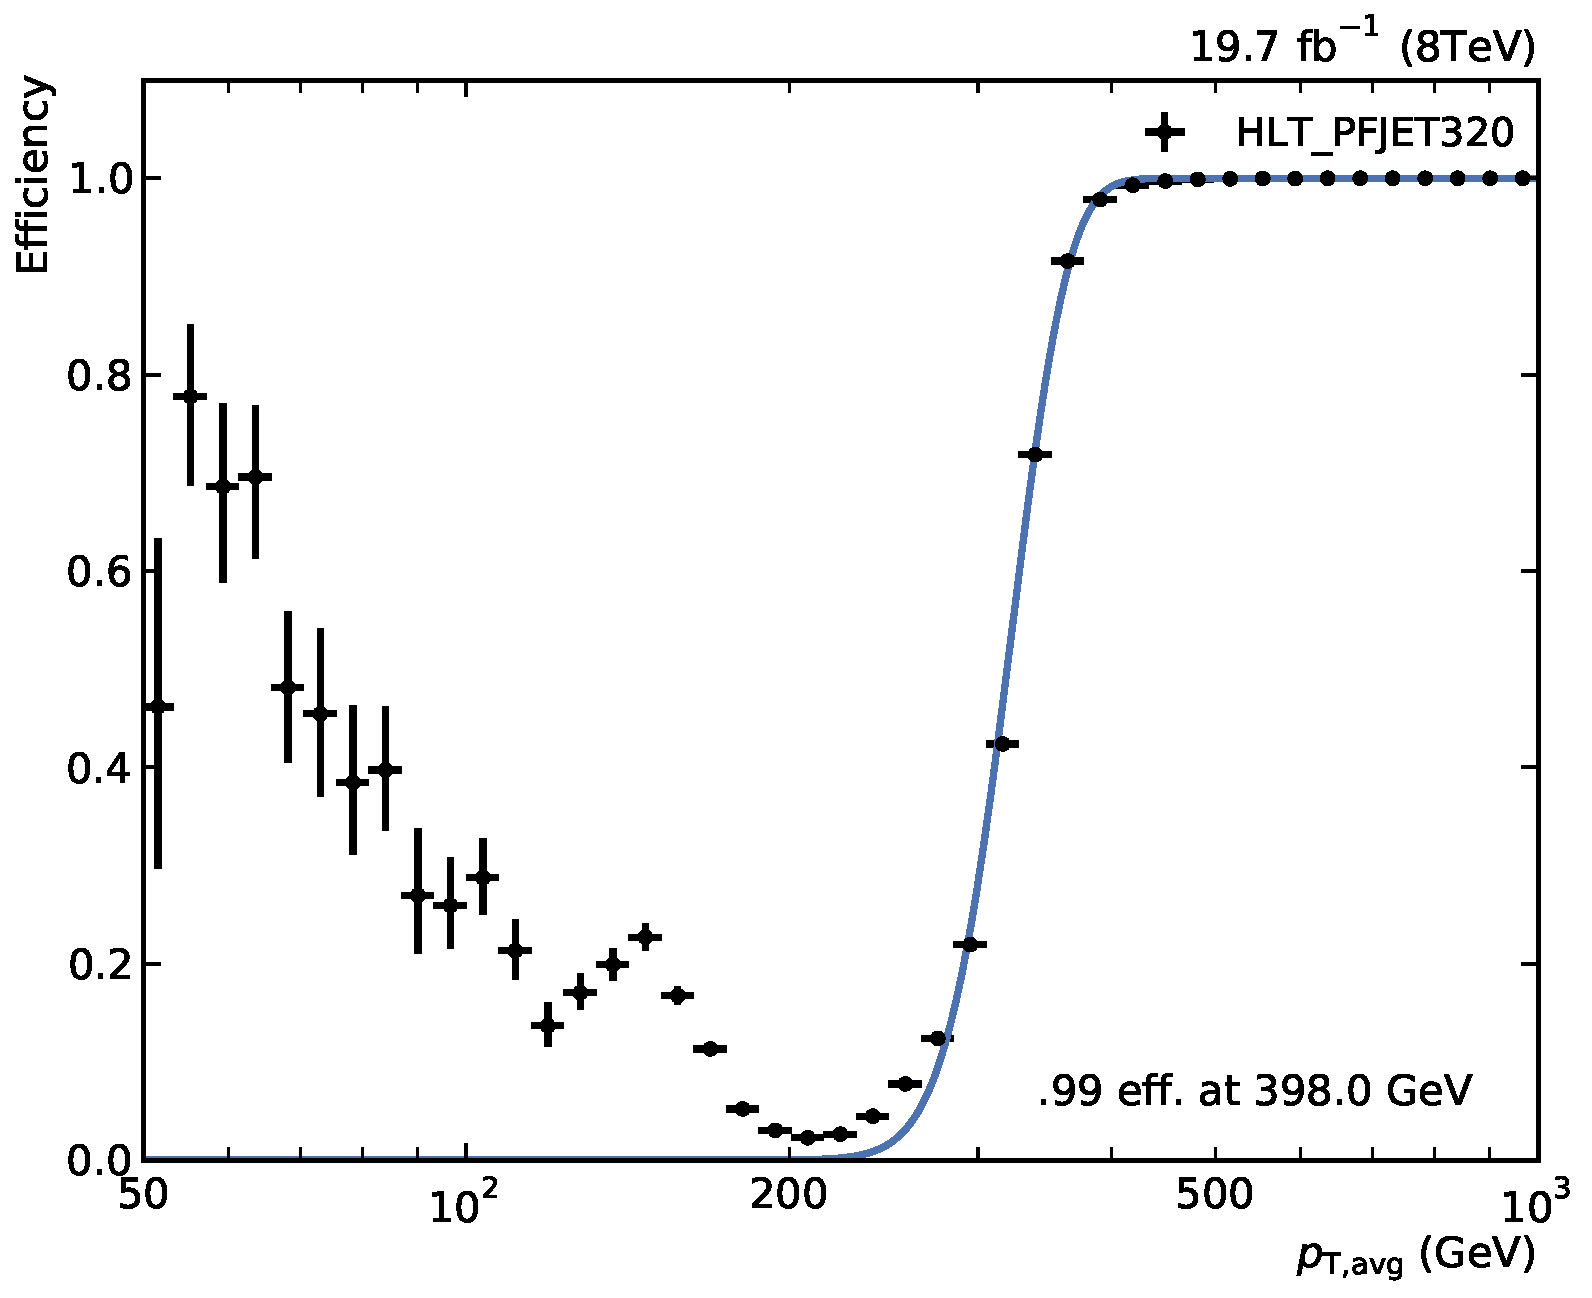
\includegraphics[width=0.49\textwidth]{figures/measurement/trigger_eff_HLT_PFJET320_default.pdf}\hfill
    \caption[Turn-on curves of single jet HLT trigger paths]{Trigger turn-on curves for the single jet trigger
    paths used in the analysis. To determine the 99\% efficiency threshold, the
    trigger turn-on curves are fitted using a sigmoid function taking into account the
    uncertainties using Clopper-Pearson confidence intervals.}
    \label{fig:trigger_eff}
\end{figure}

The jet reconstruction algorithms and the jet energy corrections applied on HLT
level slightly differ from the ones used for the final event reconstruction.
Futhermore, the efficiency of each trigger is not calculated as a function of
jet \pt, which was used in the trigger decision, but versus \ptavg of the two
leading jets as used in this analysis. Therefore, the triggers exhibit a turn-on
behaviour, as can been seen in Fig.~\ref{fig:trigger_eff}. Consequently, it is
neccessary to determine the threshold above which a trigger becomes fully
efficient. It is defined as the value at which the efficiency is exceeds 99\%.

Basically, it is possible to calculate the efficiency of a given trigger by
dividing the number of passing events through the number of events which pass
the next-lower trigger in \pt, because by definition the looser trigger is efficient,
as soon as the higher trigger becomes efficient. This is aggravated through the
different prescales applied to each trigger path. While it is possible to
normalize the yield by the effective luminosity seen by each trigger, this
method is affected by larger statistical fluctuations as the number of events
differs strongly between the two trigger paths.

Therefore, a more challenging but superior method is employed: When the L1
and HLT triggers are processed, the jet four-vectors, on
which the trigger decision is based, are stored. Thus, it is possible to
recalculate the trigger decision by comparing the transverse momentum of the L1
trigger object with the L1 threshold and the \pt of the HLT trigger object with
the HLT threshold~\cite{Stober:2012abc}.

Similarly, the trigger decision of the next higher trigger can be emulated
starting from a lower trigger path. A set of events $S_1 = \left\{E_i | T_A
(E_i) = \mathrm{true} \right\}$ which was accepted  by the lower trigger path $T_A$ is
used to determine the subset $S_2 = \left\{E_i|T_A(E_i) \wedge  T_B(E_i)
\right\}$ which also passes the next higher trigger $T_B$, see
Eq.~\ref{eq:trigger_eff}. The quotient of both event sets is used to determine
the turn-on curve as shown for each trigger path in Fig.~\ref{fig:trigger_eff}. 
The uncertainty on the efficiency is
indicated by error bars which represent Clopper-Pearson confidence intervals.

\begin{equation}
\label{eq:trigger_eff}
    f_{\mathrm{eff}} (x) = \frac{N(\left\{E_i|T_A(E_i) \wedge T_B(E_i), x)\right\}}{N(\left\{ E_i | T_A(E_i) = \mathrm{true} \right\} , x)}
\end{equation}

To determine the point, at which the trigger efficiency is larger than 99\%, the
turn-on distribution is fitted using a sigmoid function, that describes the
turn-on behaviour of the trigger paths.

\begin{equation}
\label{eq:trigger_eff_fit}
    f_{\mathrm{fit}} (x) = \frac{1}{2} \left( 1 + \erf \left(\frac{x-\mu}{\sqrt{2}\sigma}\right)\right)
\end{equation}

The thresholds which were finally used in the data analysis deviate slightly
from the ones shown in Figure~\ref{fig:trigger_eff} as each trigger threshold
was measured separately in each \ystar and \yboost bin respectively and the most
conservative, thus the highest threshold, is finally chosen. They are given in
Table~\ref{tab:triggers}

It has to be mentioned, that there are also HLT triggers available which
specifically trigger on the average transverse momentum of the dijet system.
These were implemented for dijet calibration purposes. Naturally, they appear to
be the better choice also for this analysis. The \ptavg trigger paths were studied,
but the performance is only comparable and partially even slightly worse due to
larger prescales applied to these trigger paths which result in larger
statistical uncertainties compared to the single jet trigger paths.

\subsection{Primary Vertex Selection}

The cuts on the primary vertices further reject beam background and off-centre bunch
crossings. Each event has to contain at least one primary vertex (PV) which is well
reconstructed within a distance of $|z_\mathrm{PV}| < \SI{24}{\centi \meter}$ to
the nominal interaction point of the detector. Futhermore, the radial distance
$\rho_\mathrm{PV}$ needs to be smaller than $\SI{2}{\centi\meter}$. To
ensure a high quality of the vertex reconstruction in the fit, the number of
degrees of freedom in the vertex fit, $n_{\mathrm{dof,PV}}$ needs to be at least
four. Consequently, at least four tracks need to be present in order to
perform a valid vertex fit.

\subsection{Missing transverse energy cut}

If all particles could be identified and perfectly measured, the transverse
momentum of all particles would sum up to zero. The imbalance in the transverse
momentum of all visible particles, which can be measured in the detector is
called the missing transverse momentum (MET). Neutrinos, for example, leave the
detector undetected and do contribute to the MET. MET is an important ingredient
in many measurements involving W bosons, top quarks or searches for physics
beyond the standard model which involve undetectable particles. 

\begin{figure}[htbp]
    \centering
    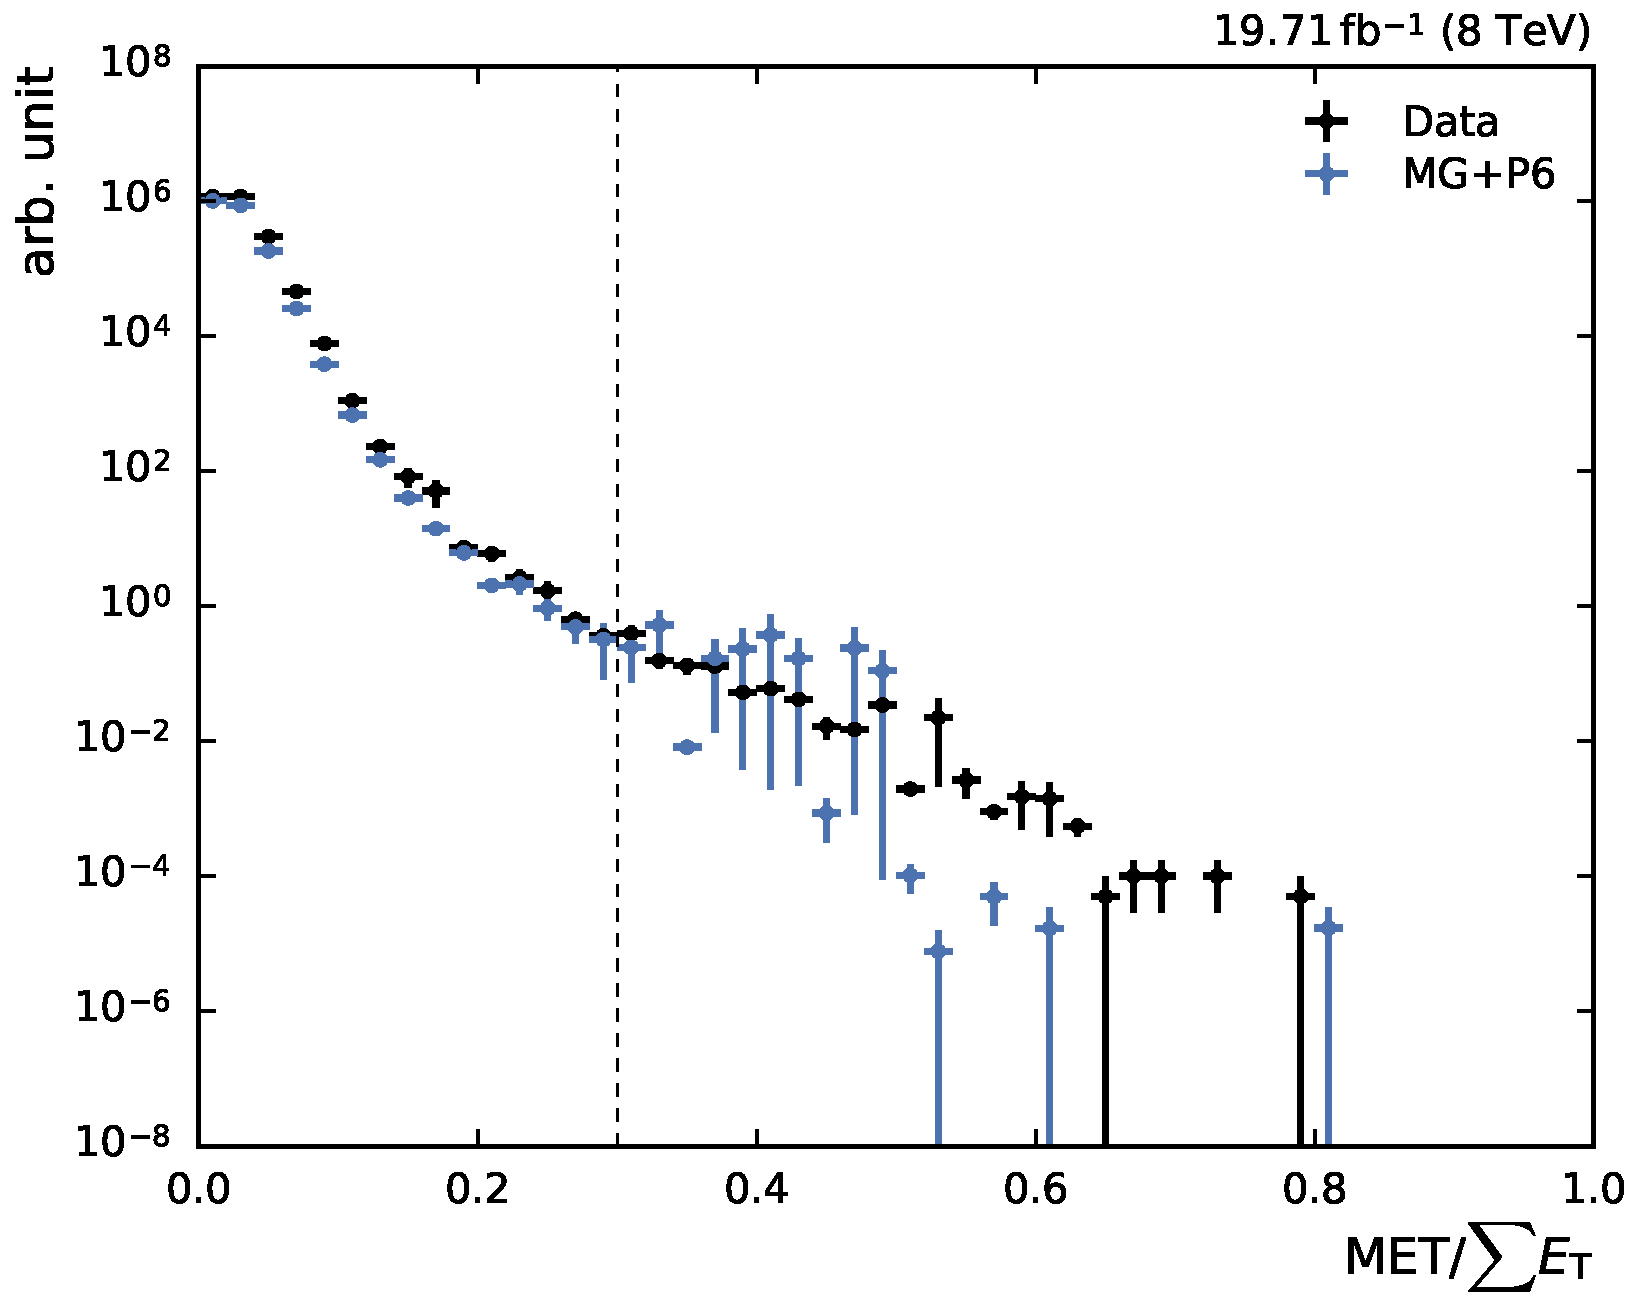
\includegraphics[width=0.7\textwidth]{figures/measurement/metoversumet.pdf}
    \caption[Missing transverse energy distribution]{Missing transverse energy
    fraction of the total transverse energy per event in data and simulated
    events. To remove background and noise, events with a fraction exceeding a
    threshold are rejected. }
    \label{fig:mc:met_fraction}
\end{figure}

However, a large fraction of MET in an event is not always caused by physics
processes. Very often, the reason can be found in detector noise, cosmic rays or
beam-halo particles. Therefore, a sequence of algorithms developed by the MET
working group at CMS~\cite{jetmet:metfilters}, is employed which identifies and
rejects these events.  Moreover, a cut is applied which removes events in which
the missing transverse energy fraction \met constitutes a large fraction of the
total transverse energy $\sum_i E_{\mathrm{T},i}$, see
Fig.~\ref{fig:mc:met_fraction},

\begin{equation}
    \frac{\met}{\sum_i E_{\mathrm{T},i}} < 0.3.
\end{equation}

\subsection{Jet Identification}

The jet identification criteria (jet ID) rejects noise and noise-enhanced jets
while all real jets are kept. The jet ID is not applied event-wise, but each jet
is accepted or removed from the list of valid jets. The algorithm works on
reconstructed jets using information of the clustered particle candidates.
Following the official recommendations of the \textsc{JetMET}
group~\cite{jetmet:jetid}, the loose jet ID is used. All jets passing the jet ID
are then further processed in the analysis chain. 

The properties of the reconstructed jets and their respective cuts are listed in
Table~\ref{tab:jetid}. The cut on the fraction of neutral hadrons and photons
removes HCAL noise and ECAL noise, respectively. Muons, that are falsely
identified and clustered as jets are removed by the muon fraction criterion.
Based on information of the tracker, additional selection cuts are enforced in
the region $|\eta| < 2.4$. Fake jets clustered from electrons are removed by the
charged electromagnetic fraction cut. Furthermore, the fraction of charged hadrons in the
jet must be larger than zero. This cut is important since the CHS algorithm
removes charged particles from pileup vertices. Consequently, jets without any
charged hadrons are very likely to be pileup jets. The
Figs.~\ref{fig:jet_constituents_fractions} and~\ref{fig:jet_constituents_counts}
show the distributions of the jet constituents observed in data and simulated
events.

\begin{figure}[htbp]
    \centering
    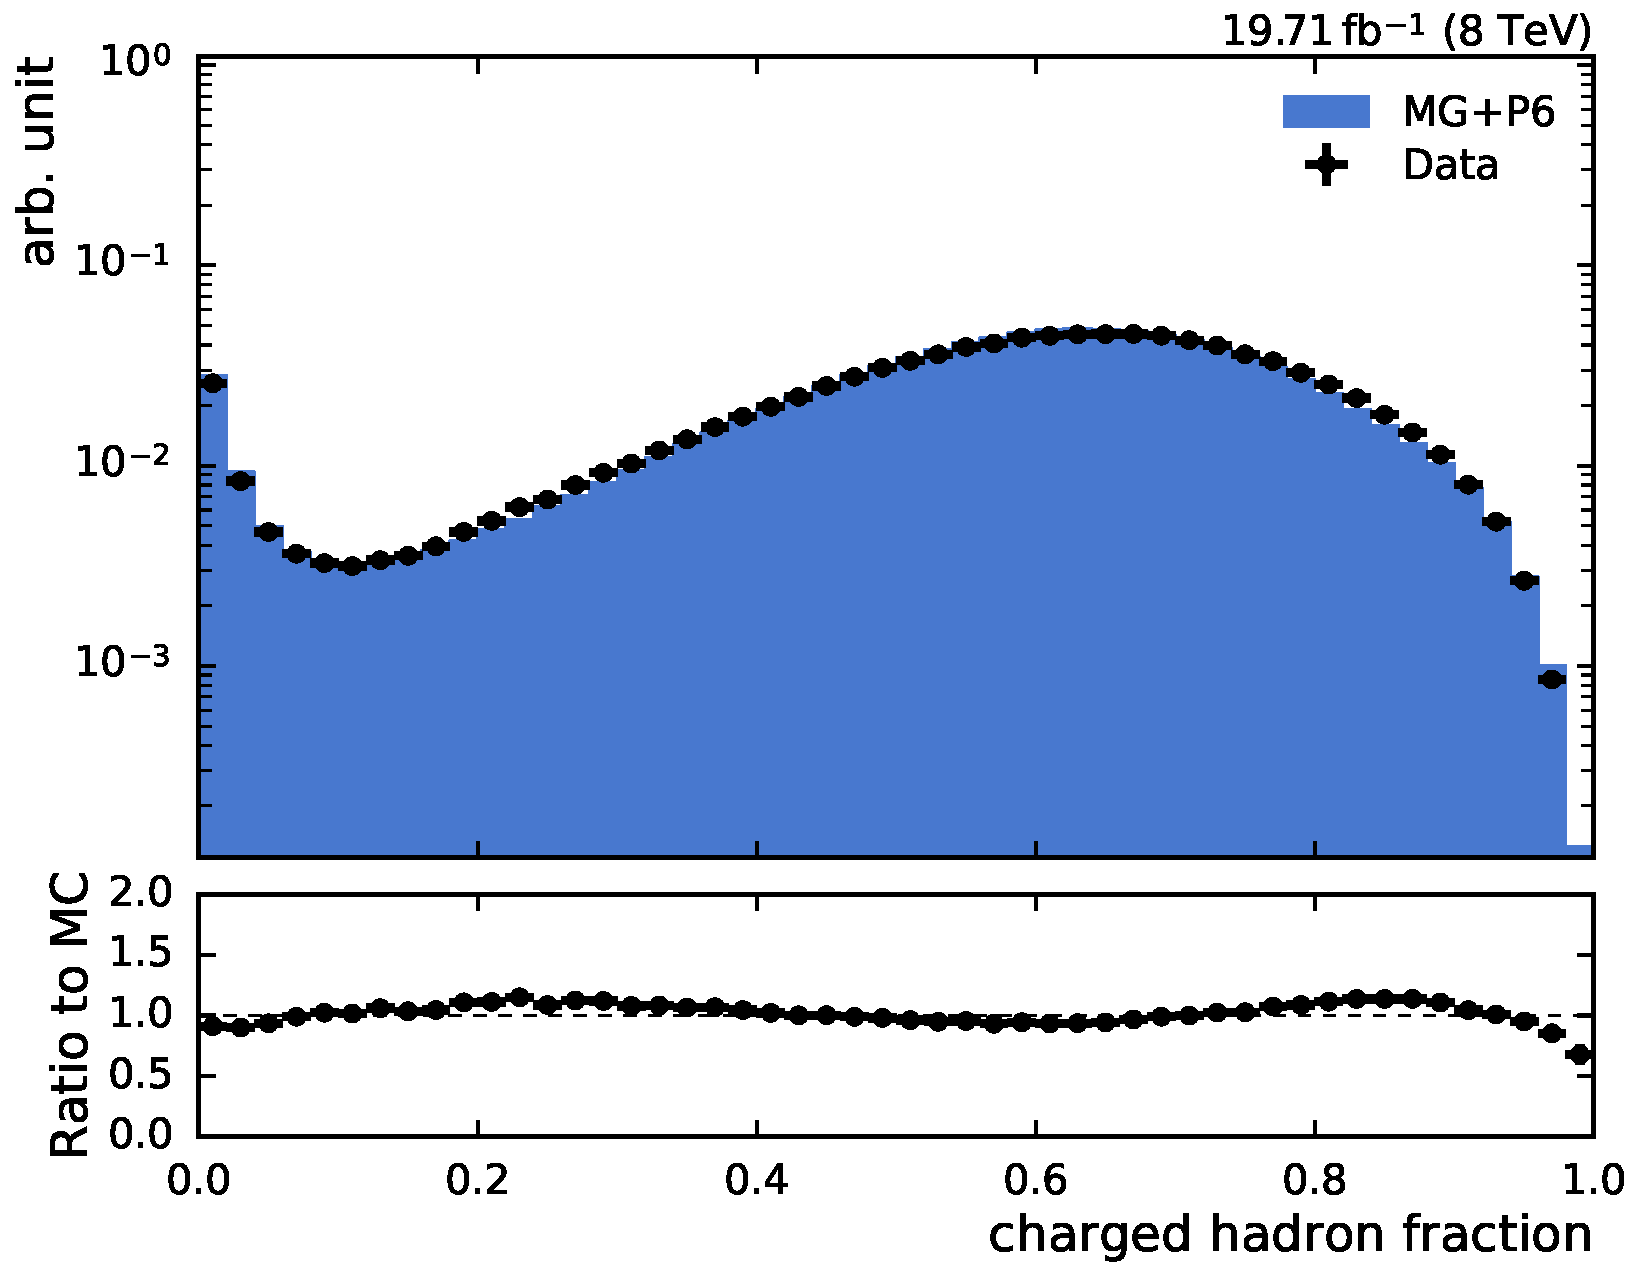
\includegraphics[width=0.49\textwidth]{figures/measurement/jet_constituent_chargedHadronFraction.pdf}\hfill
    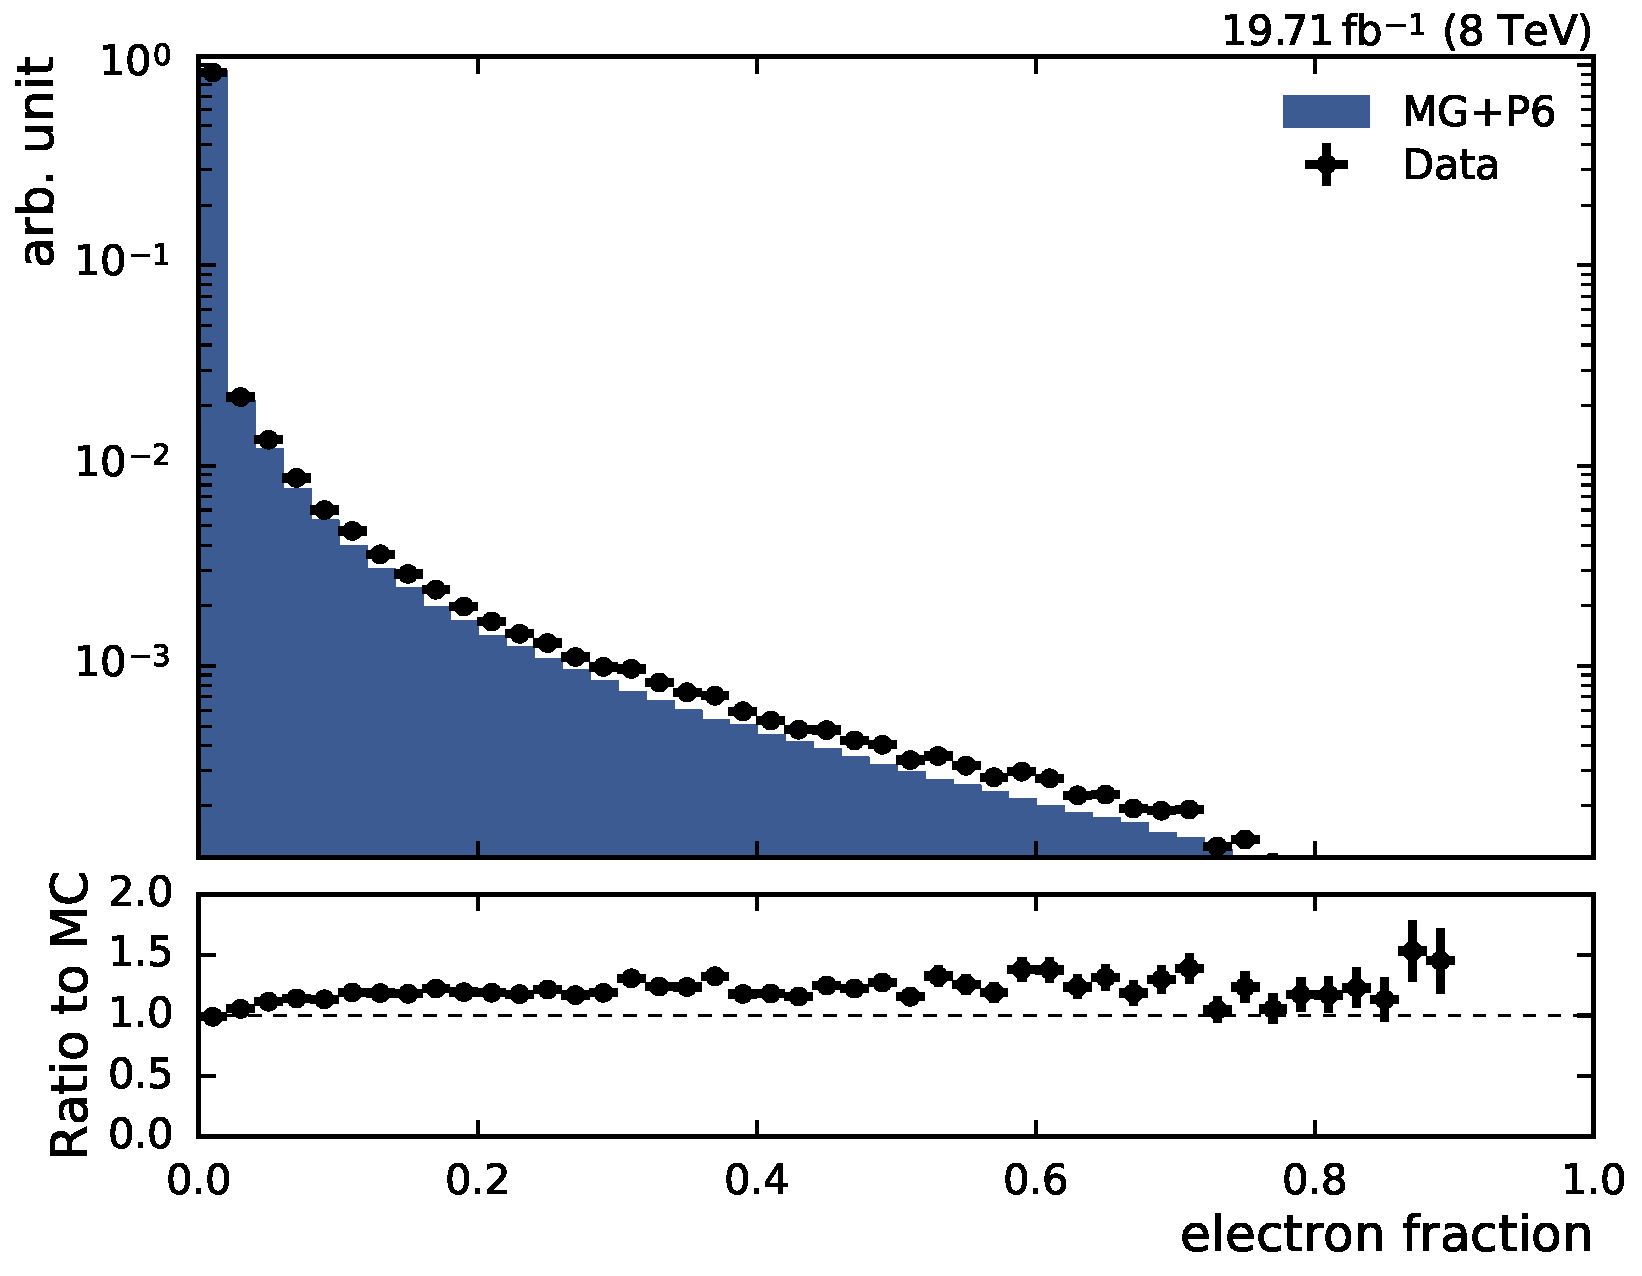
\includegraphics[width=0.49\textwidth]{figures/measurement/jet_constituent_electronFraction.pdf}
    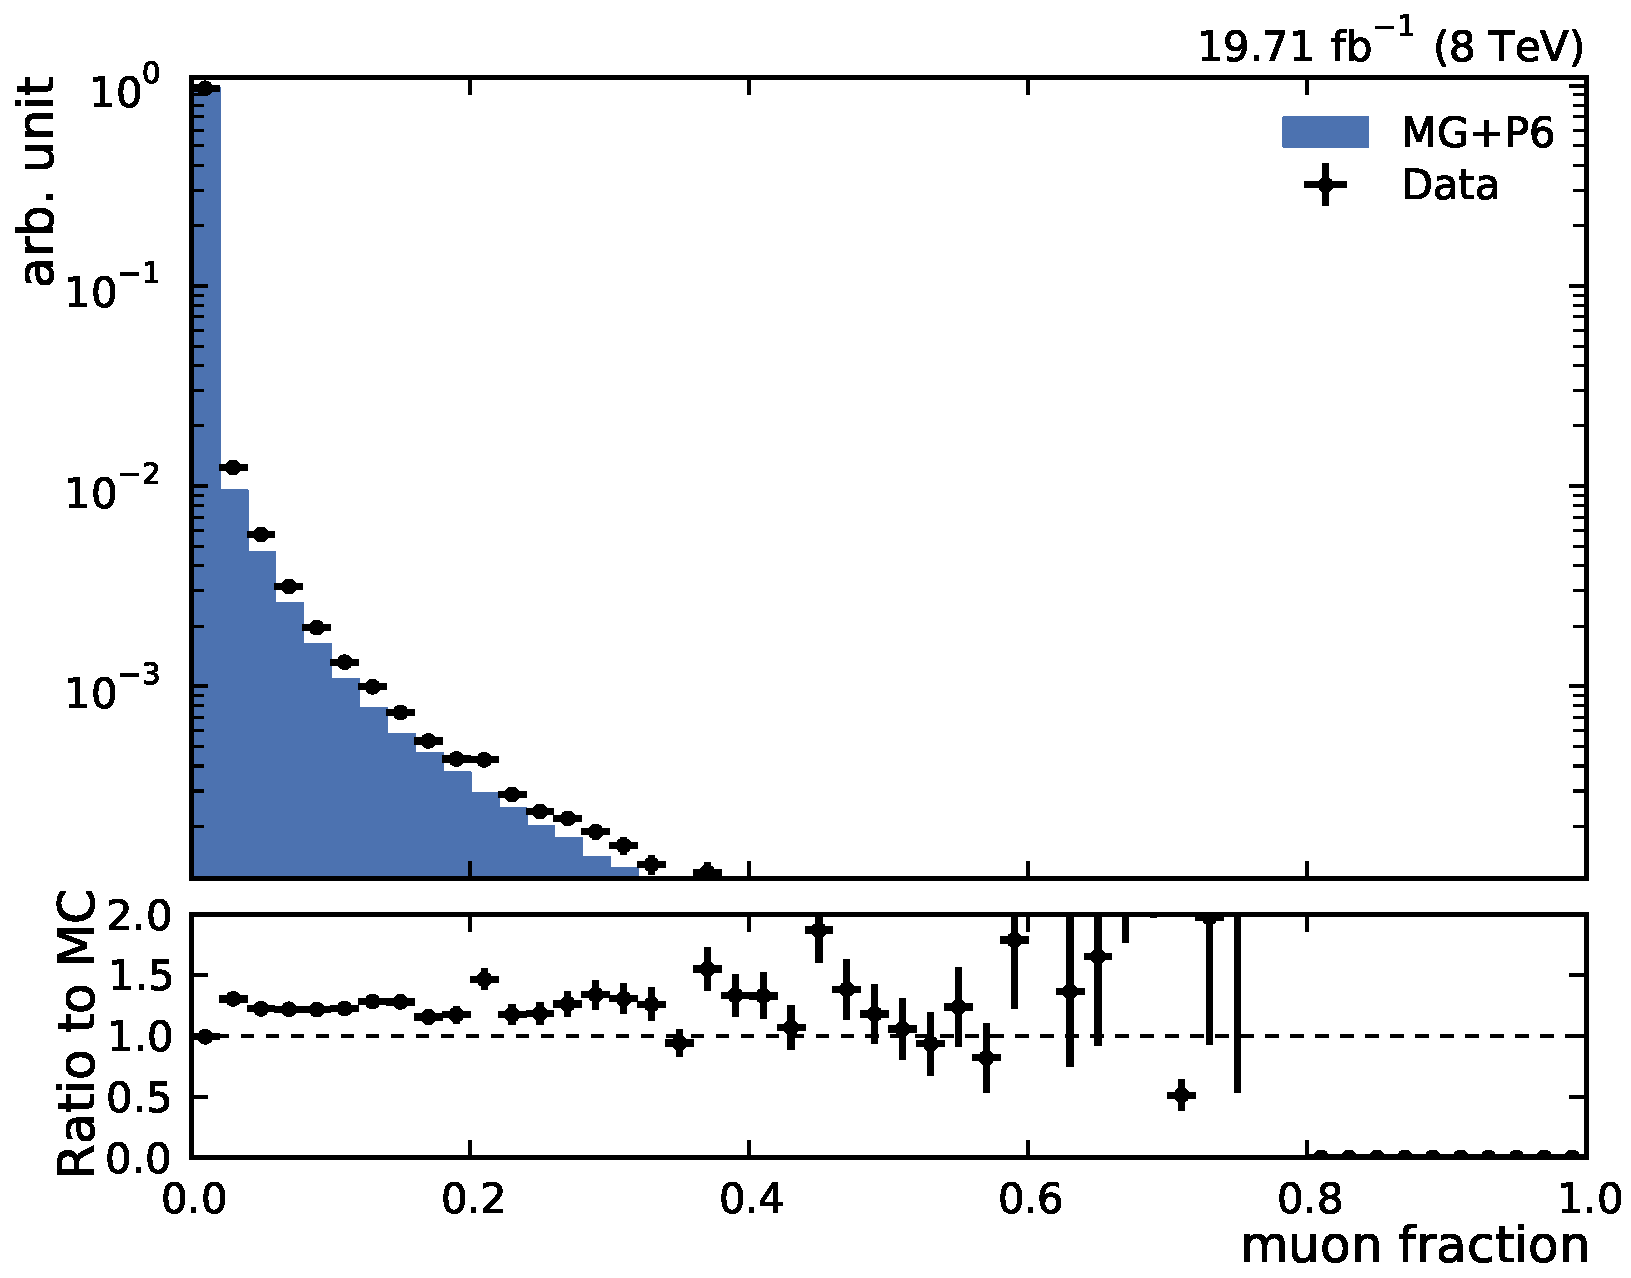
\includegraphics[width=0.49\textwidth]{figures/measurement/jet_constituent_muonFraction.pdf}\hfill
    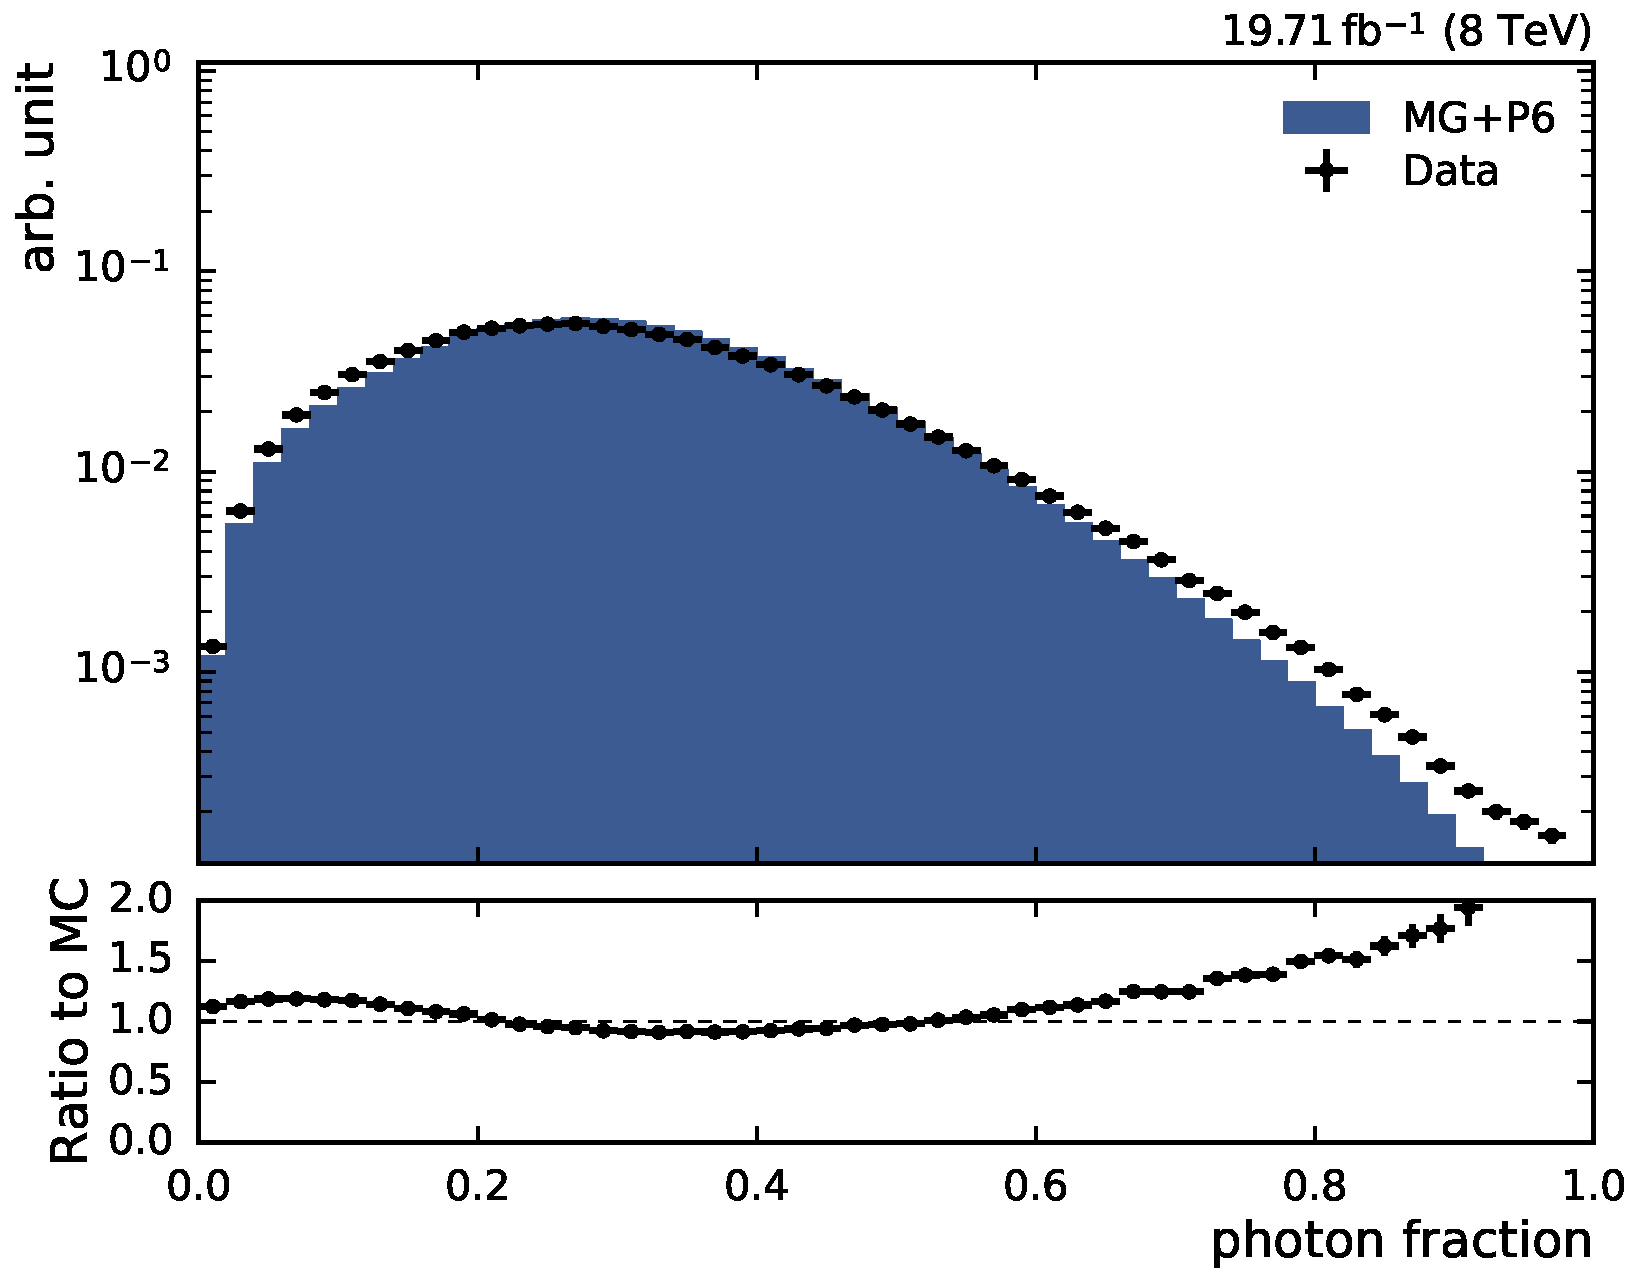
\includegraphics[width=0.49\textwidth]{figures/measurement/jet_constituent_neutralEMFraction.pdf}
    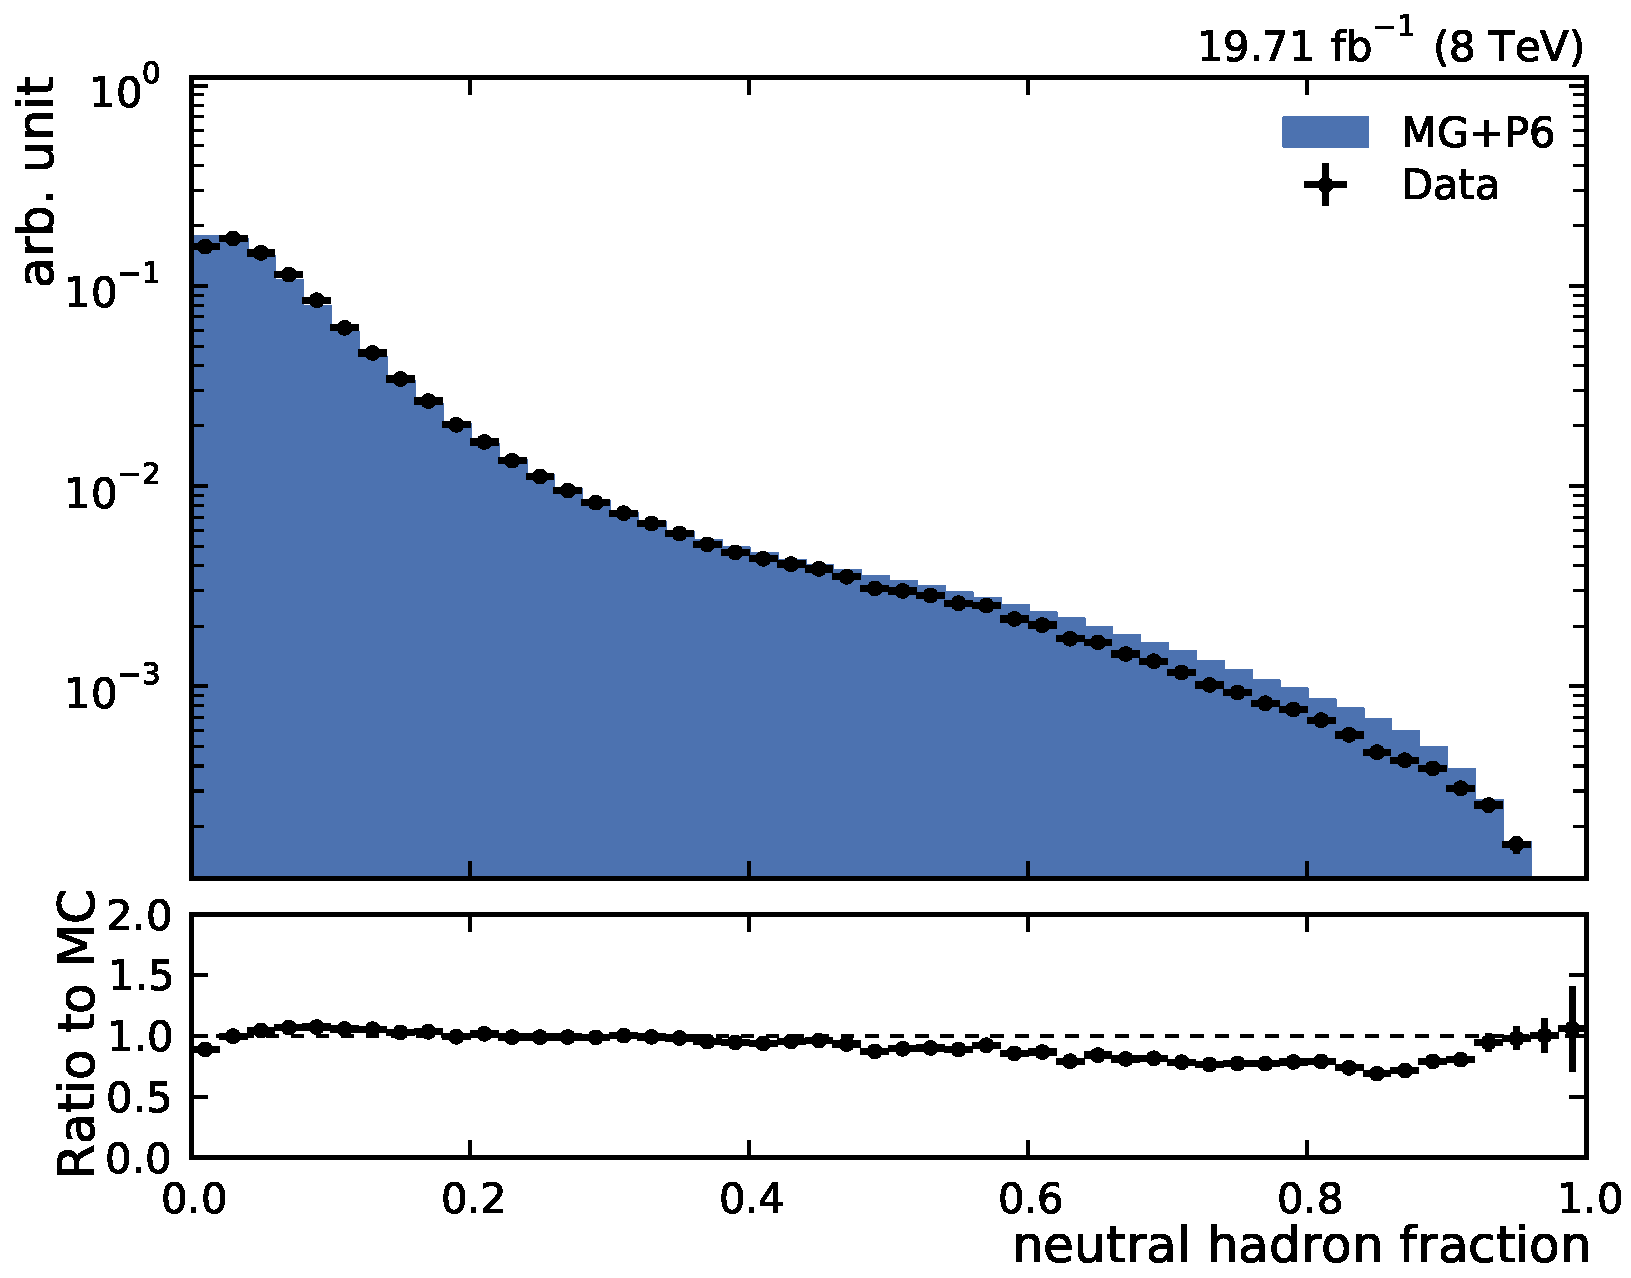
\includegraphics[width=0.49\textwidth]{figures/measurement/jet_constituent_neutralHadronFraction.pdf}
    \caption[PF candidate fractions in jets]{The fractions of jet constituents as
            observed in data and simulated events for different types of PF candidates.
            Data and simulation are normalized to the same number of events.}
    \label{fig:jet_constituents_fractions}
\end{figure}

\begin{figure}[htbp]
    \centering
    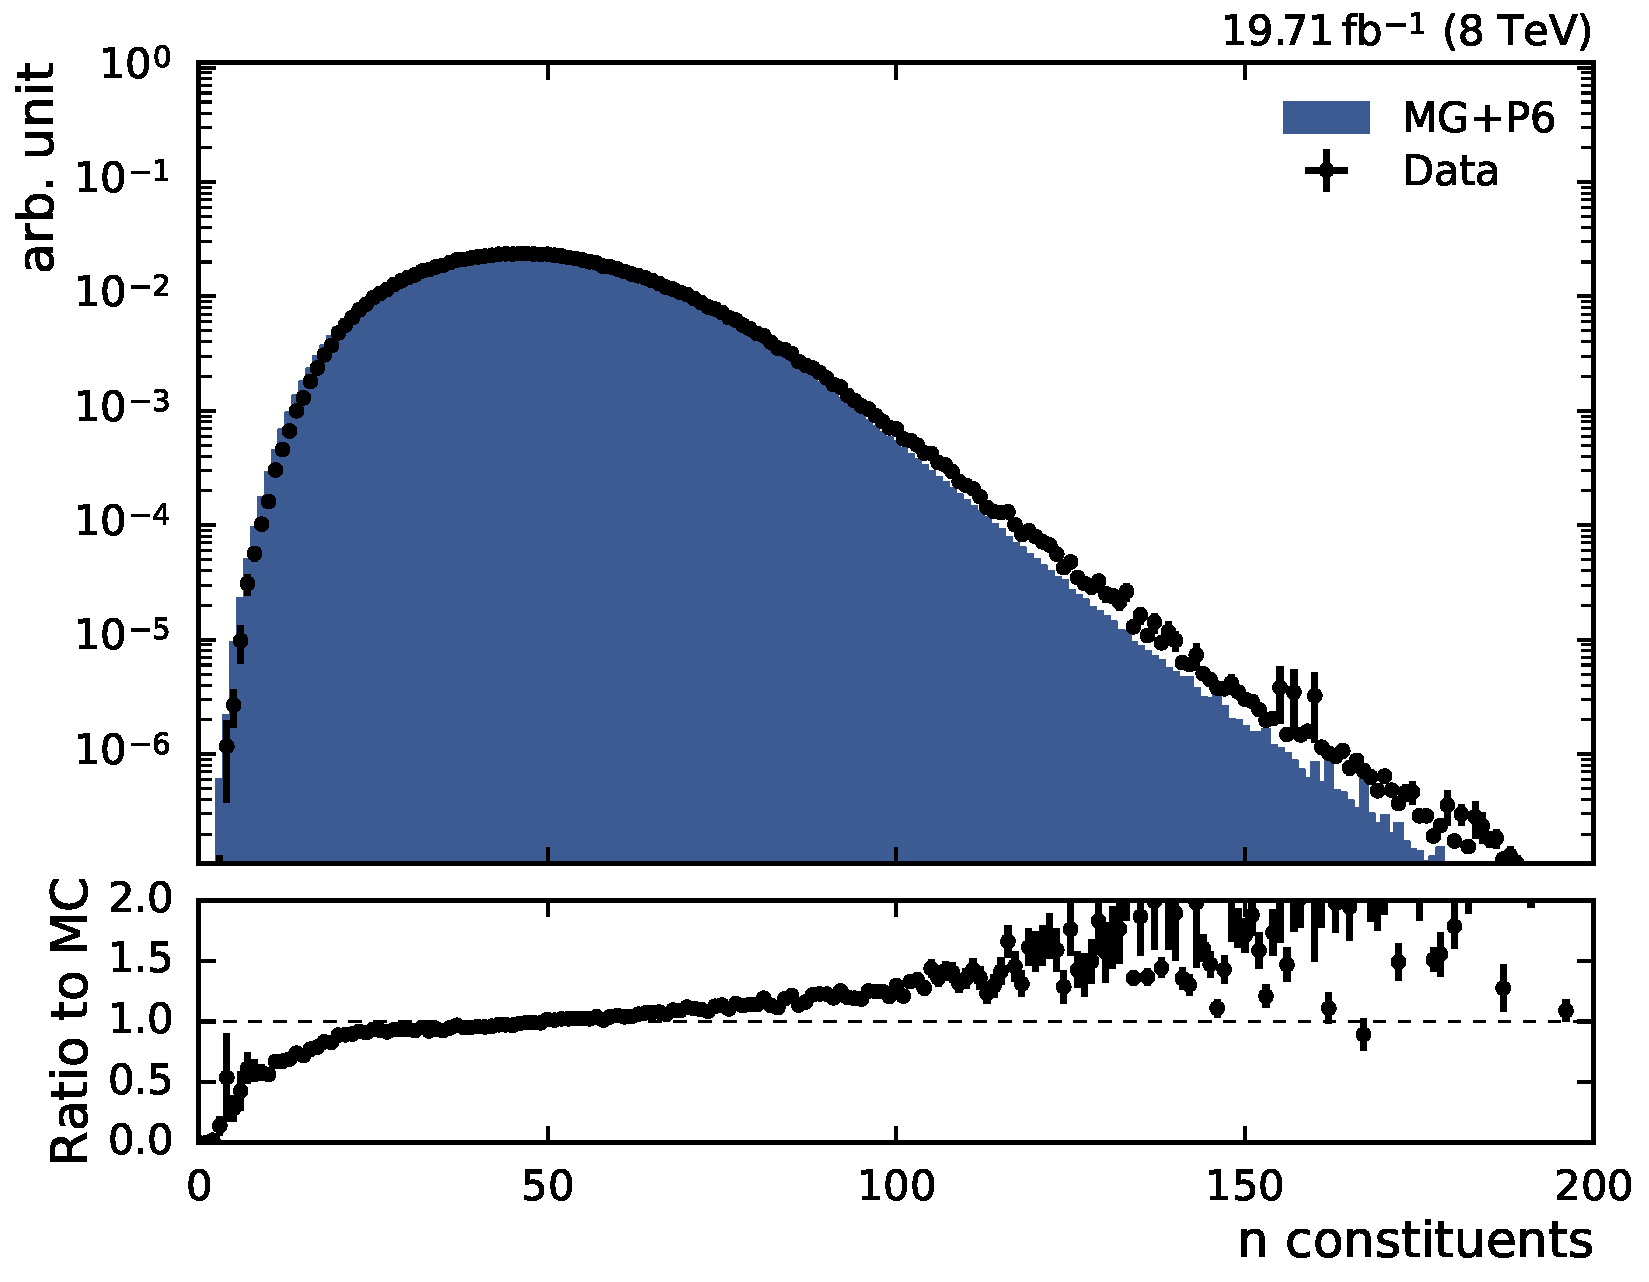
\includegraphics[width=0.49\textwidth]{figures/measurement/jet_constituent_nConstituents.pdf}\hfill
    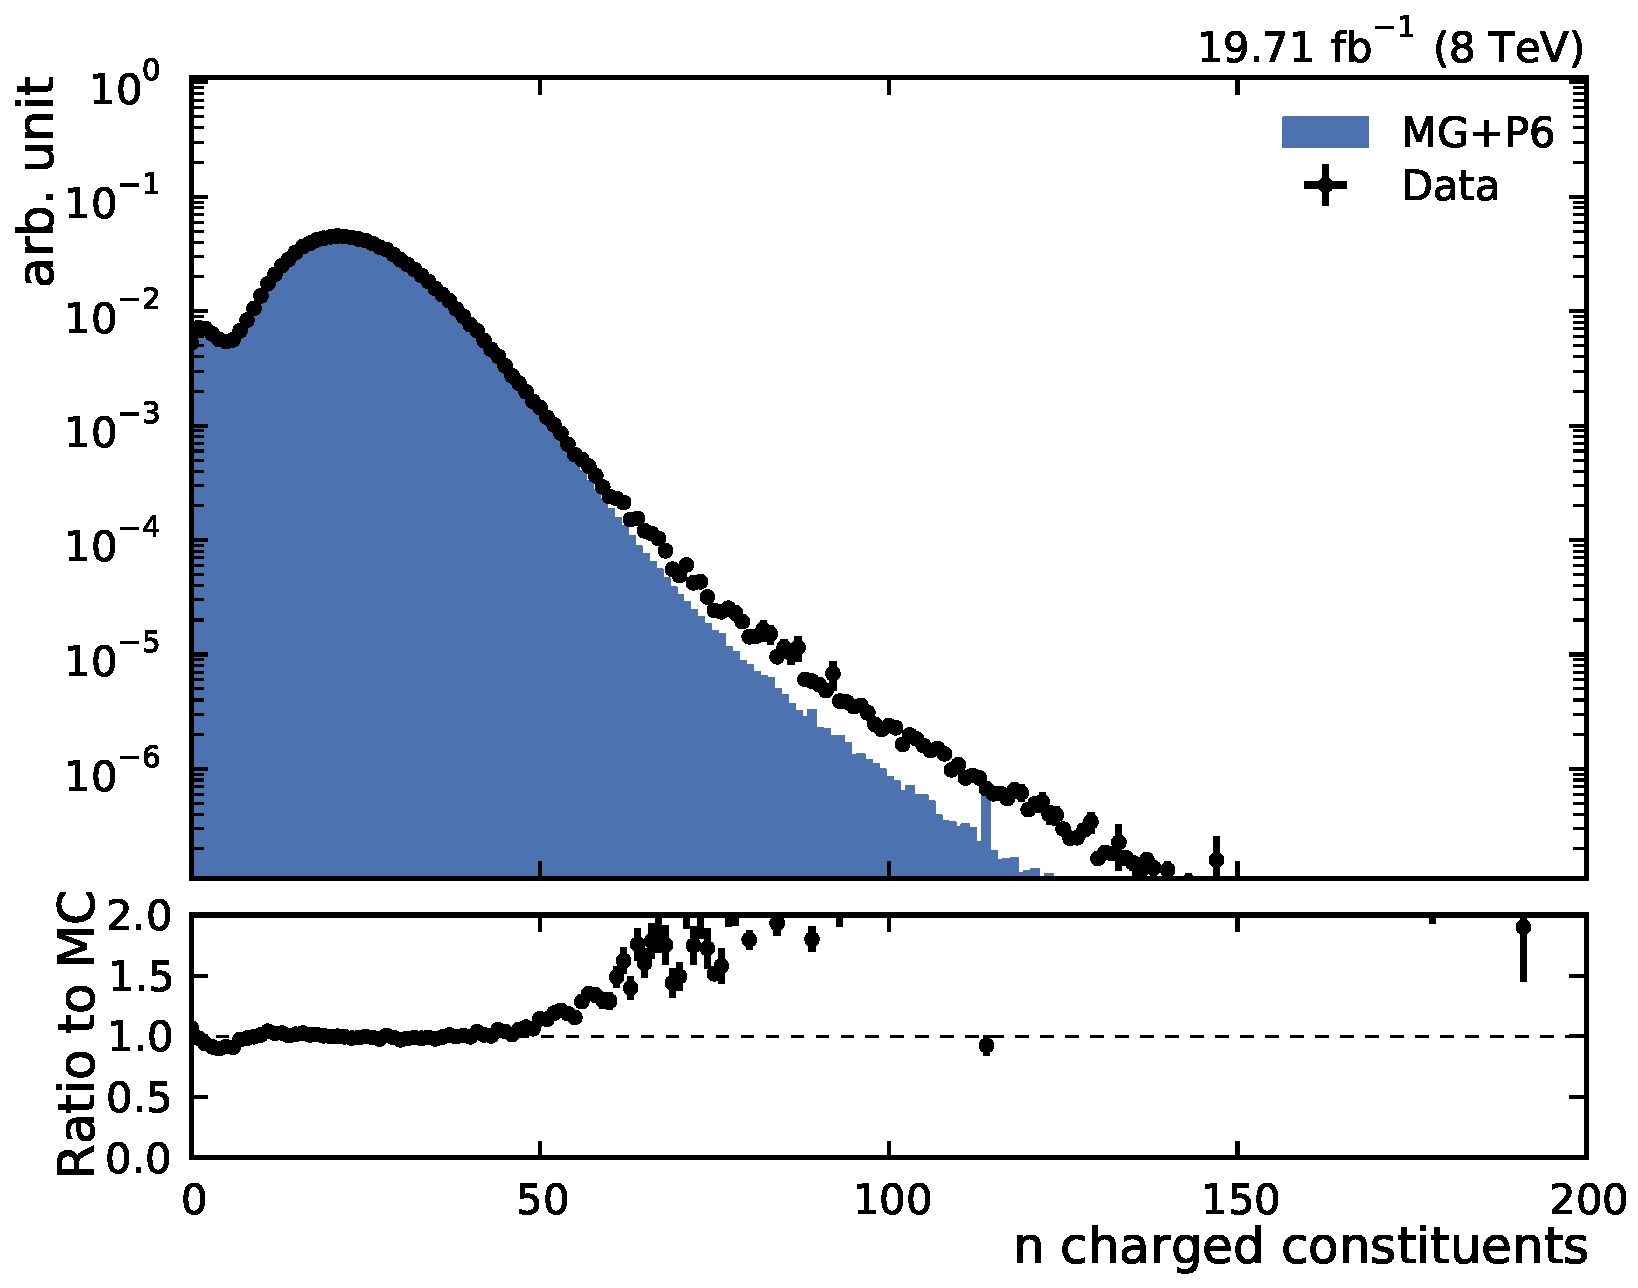
\includegraphics[width=0.49\textwidth]{figures/measurement/jet_constituent_nCharged.pdf}
    \caption[Number of particle candidates in jets.]{Number of PF candidates
             clustered into a jet in data and simulated events. Data and simulation are
             normalized to the same number of events.}
    \label{fig:jet_constituents_counts}
\end{figure}

While studying the loose and tight jet criteria, it was found that the tight jet
ID removes a non-negligible fraction of jets in the forward region of the
phase space considered in this analysis. Therefore, the loose jet ID is favored
and applied in this thesis as it is also the official recommendation of the
\textsc{JetMET} group.

\begin{table}[htbp]
    \centering
    \caption[Jet ID criteria]{The jet ID removes noise and fake jets based on
        the properties of the reconstructed jets and the clustered particle
        candidates. All selection cuts which are recommended by the
        \textsc{JetMET} group are applied~\cite{jetmet:jetid}. The loose jet ID is
        used in this analysis as the tight ID removes a non-negligible fraction
        of signal events, particularly in the forward region without tracker
        coverage.}
    \label{tab:jetid}
    \begin{tabular}{llll}
    \toprule
                                 & \textbf{property}       & \textbf{loose ID} & \textbf{tight ID}\\\cmidrule(lr){2-4}
                                 \textbf{Whole $\bm{\eta}$ region} &                         &                   & \\\cmidrule(lr){1-1}
                                 & neutral hadron fraction & $< 0.99$          & $< 0.90$\\
                                 & neutral EM fraction     & $< 0.99$          & $< 0.90$\\
                                 & number of constituents  & $> 1$             & $> 1$\\
                                 & muon fraction           & $< 0.8$           & $< 0.80$\\
                                 \textbf{only $\bm{|\eta| < 2.4}$} &                         &                   & \\\cmidrule(lr){1-1}
                                 & charged hadron fraction & $> 0$             & $> 0$\\
                                 & charged multiplicity    & $> 0$             & $> 0$\\
                                 & charged EM fraction     & $< 0.99$          & $< 0.90$\\
    \bottomrule
    \end{tabular}
\end{table}


\subsection{Jet ID Efficiency}

The loose jet ID ensures a high purity of real jet events while at the same time
the efficiency is promised to be larger than 99\% for real jets. To confirm the
high selection efficiency, it is studied using a tag-and-probe technique.

Dijet events, in which the leading two jets are well balanced in $\phi$, are
selected using
\begin{equation*}
    | \Delta\phi - \pi | < 0.3
\end{equation*}
%
where $\Delta\phi$ is the azimuthal difference between the two leading jets. One of the
dijets is chosen as tag jets and has to fulfill the loose jet id. It is tested,
if the probe jet also passes the jet ID. The ratio of events in which the probe
jet also passes the criteria versus the total number of dijet events is used to
calculate the efficiency. Fig.~\ref{fig:jetid_eff} shows the efficiency as a
function of \ptavg of the dijet system for all \ystar and \yboost bins. As
promised by the \textsc{JetMET} group the efficiency is in all cases larger than
99\%.

\begin{figure}[htbp]
    \centering
    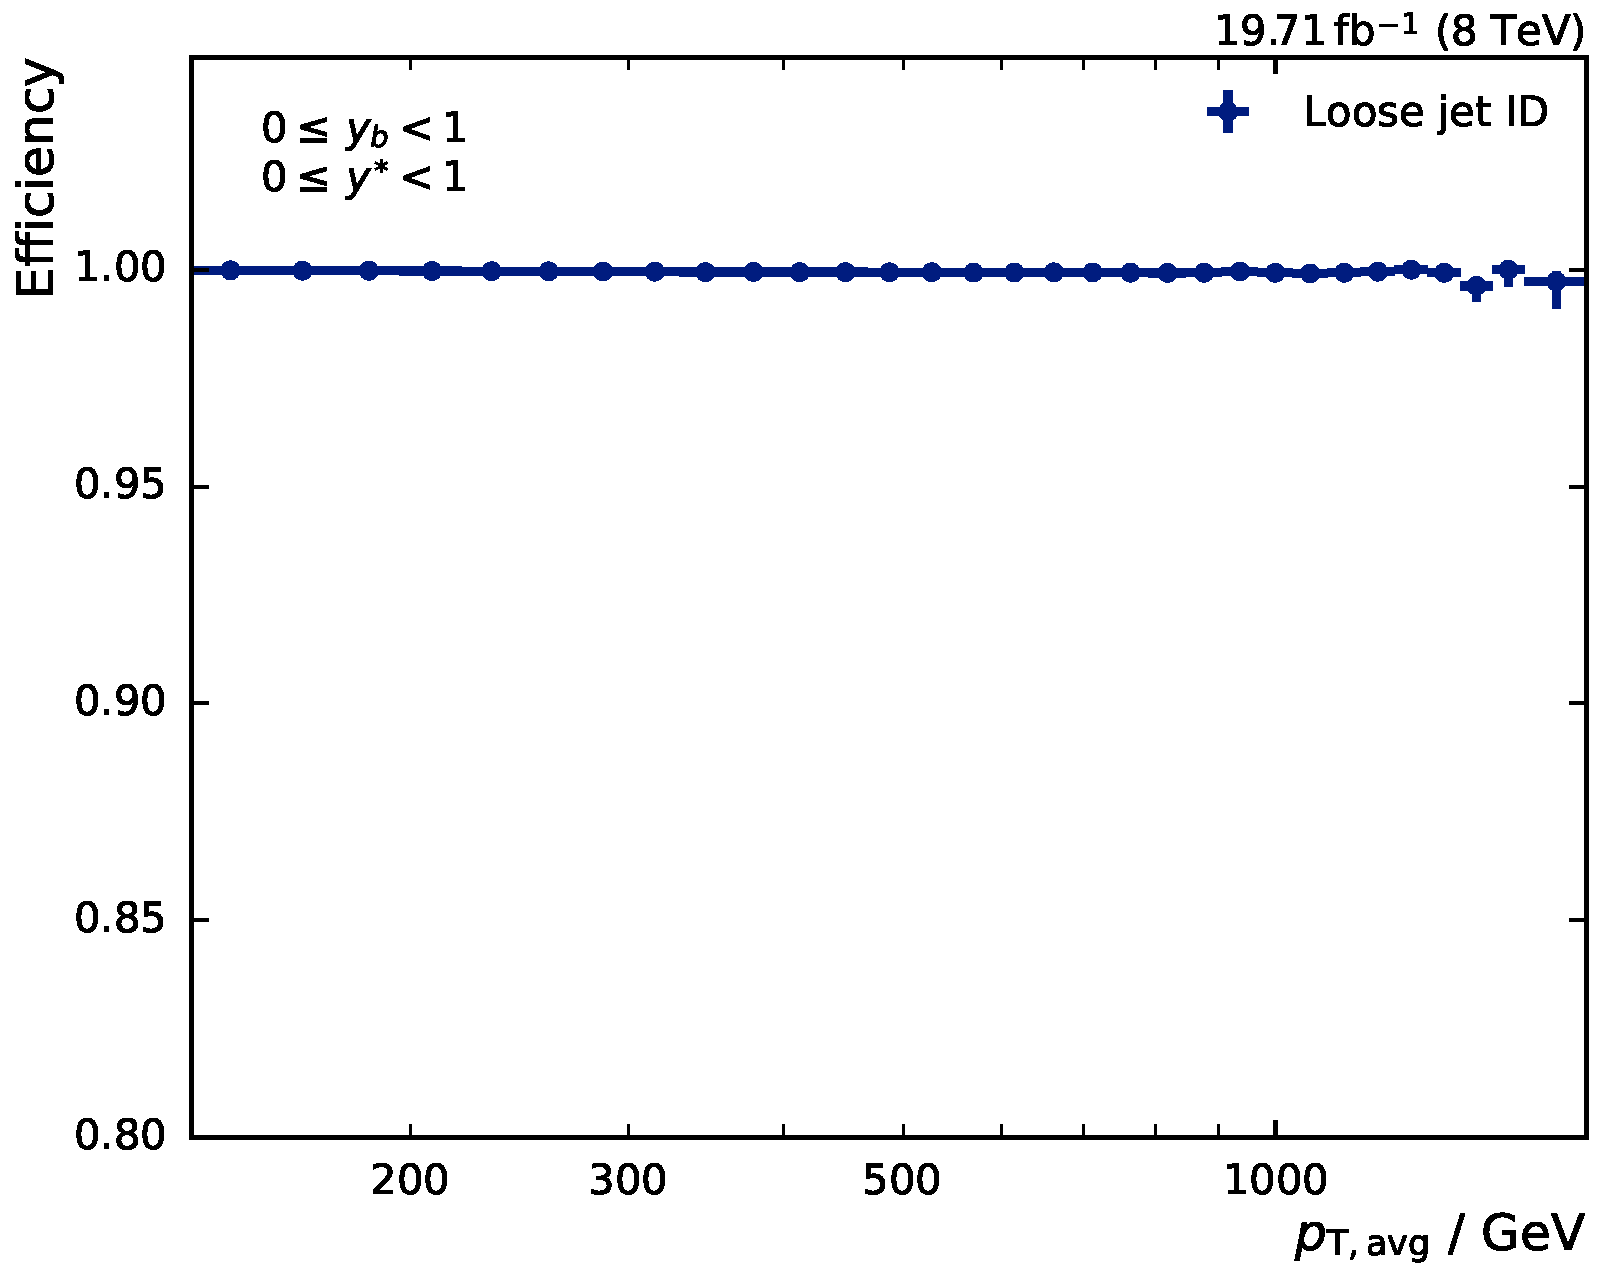
\includegraphics[width=0.49\textwidth]{figures/measurement/jetideff_yb0ys0.pdf}\hfill
    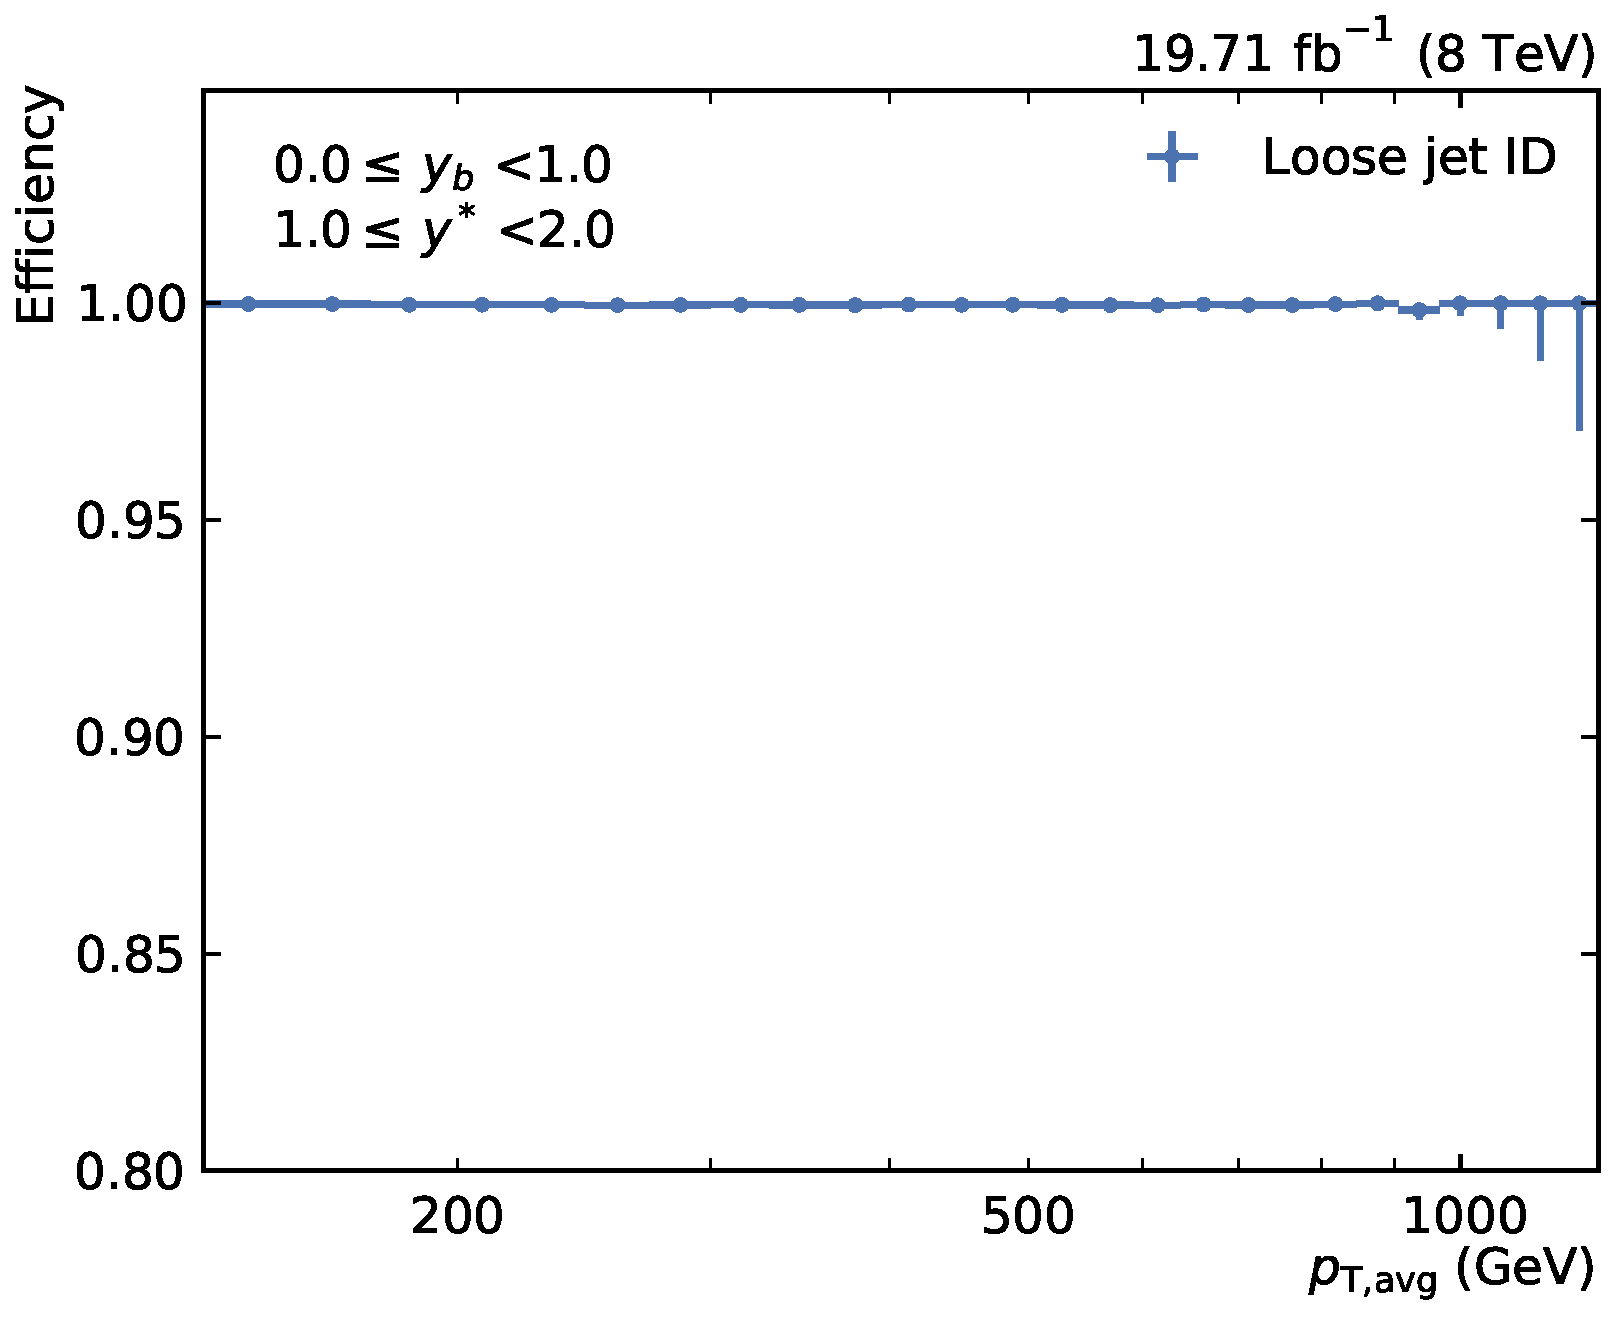
\includegraphics[width=0.49\textwidth]{figures/measurement/jetideff_yb0ys1.pdf}
    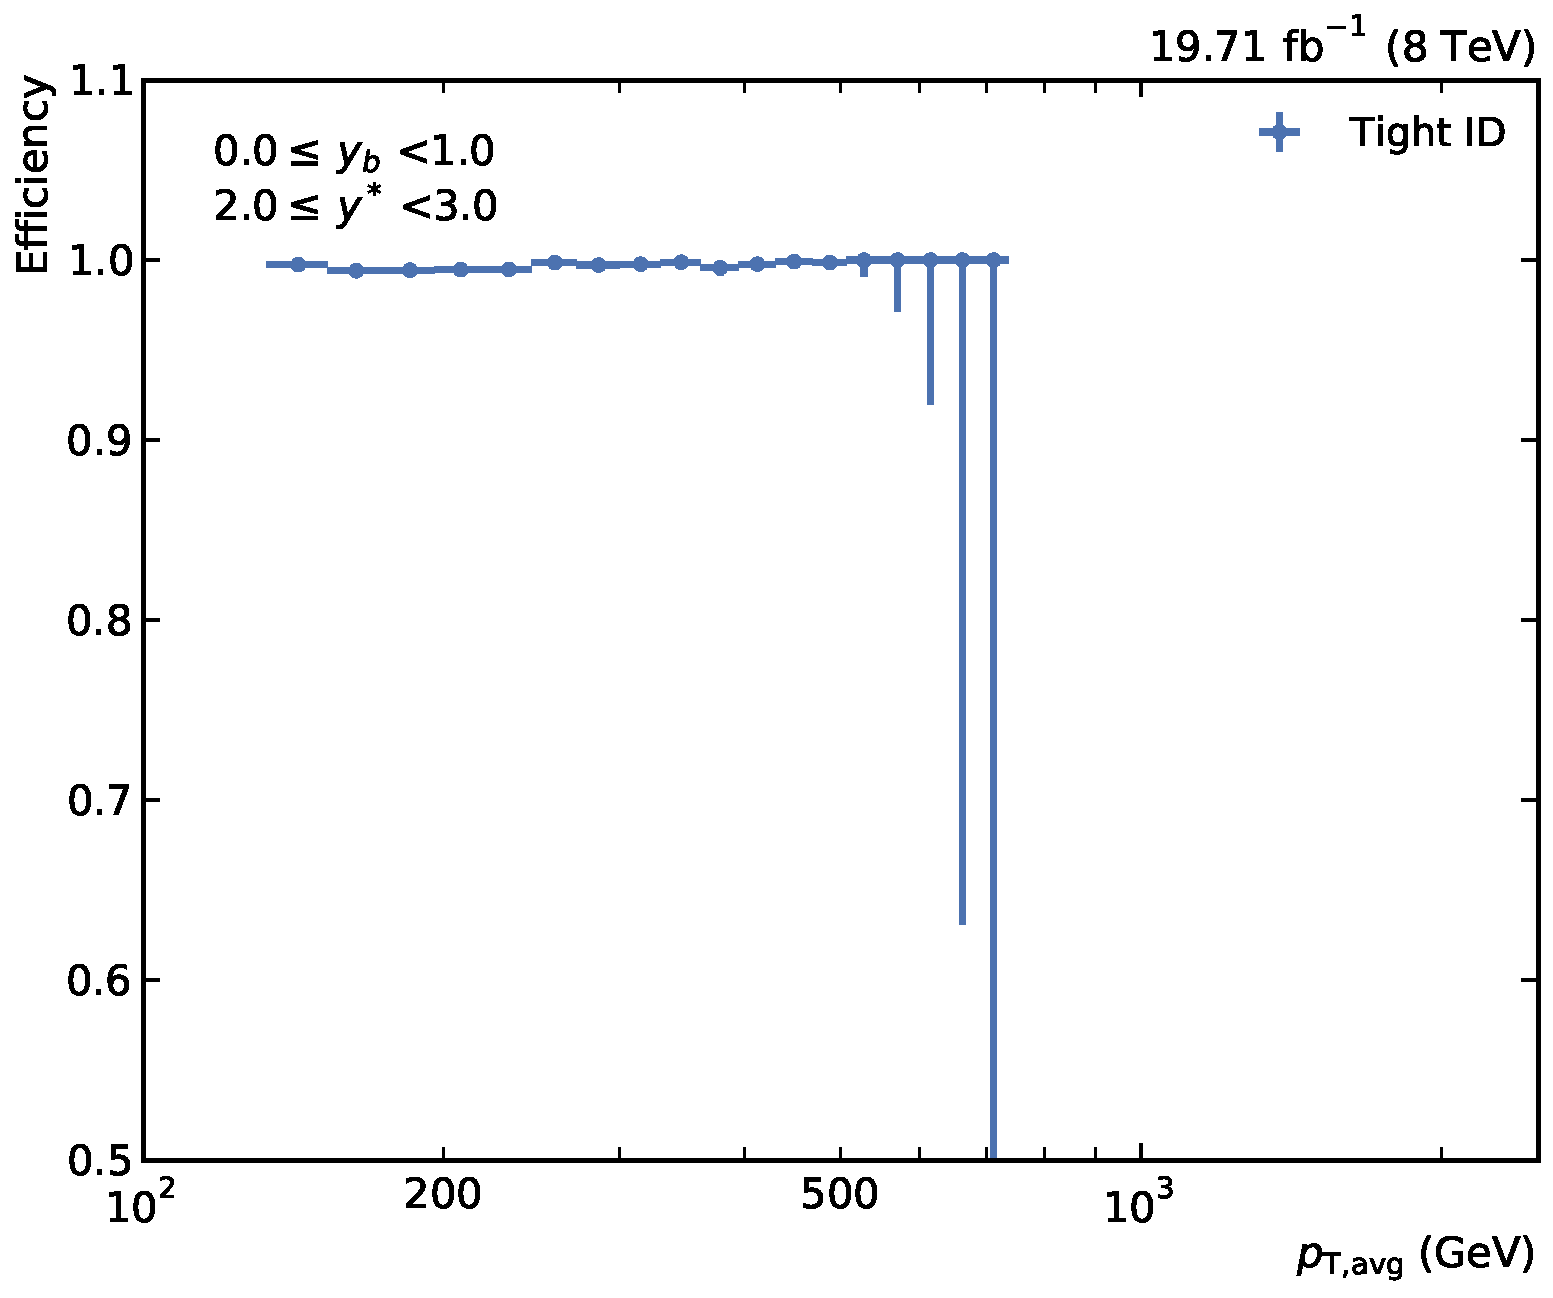
\includegraphics[width=0.49\textwidth]{figures/measurement/jetideff_yb0ys2.pdf}\hfill
    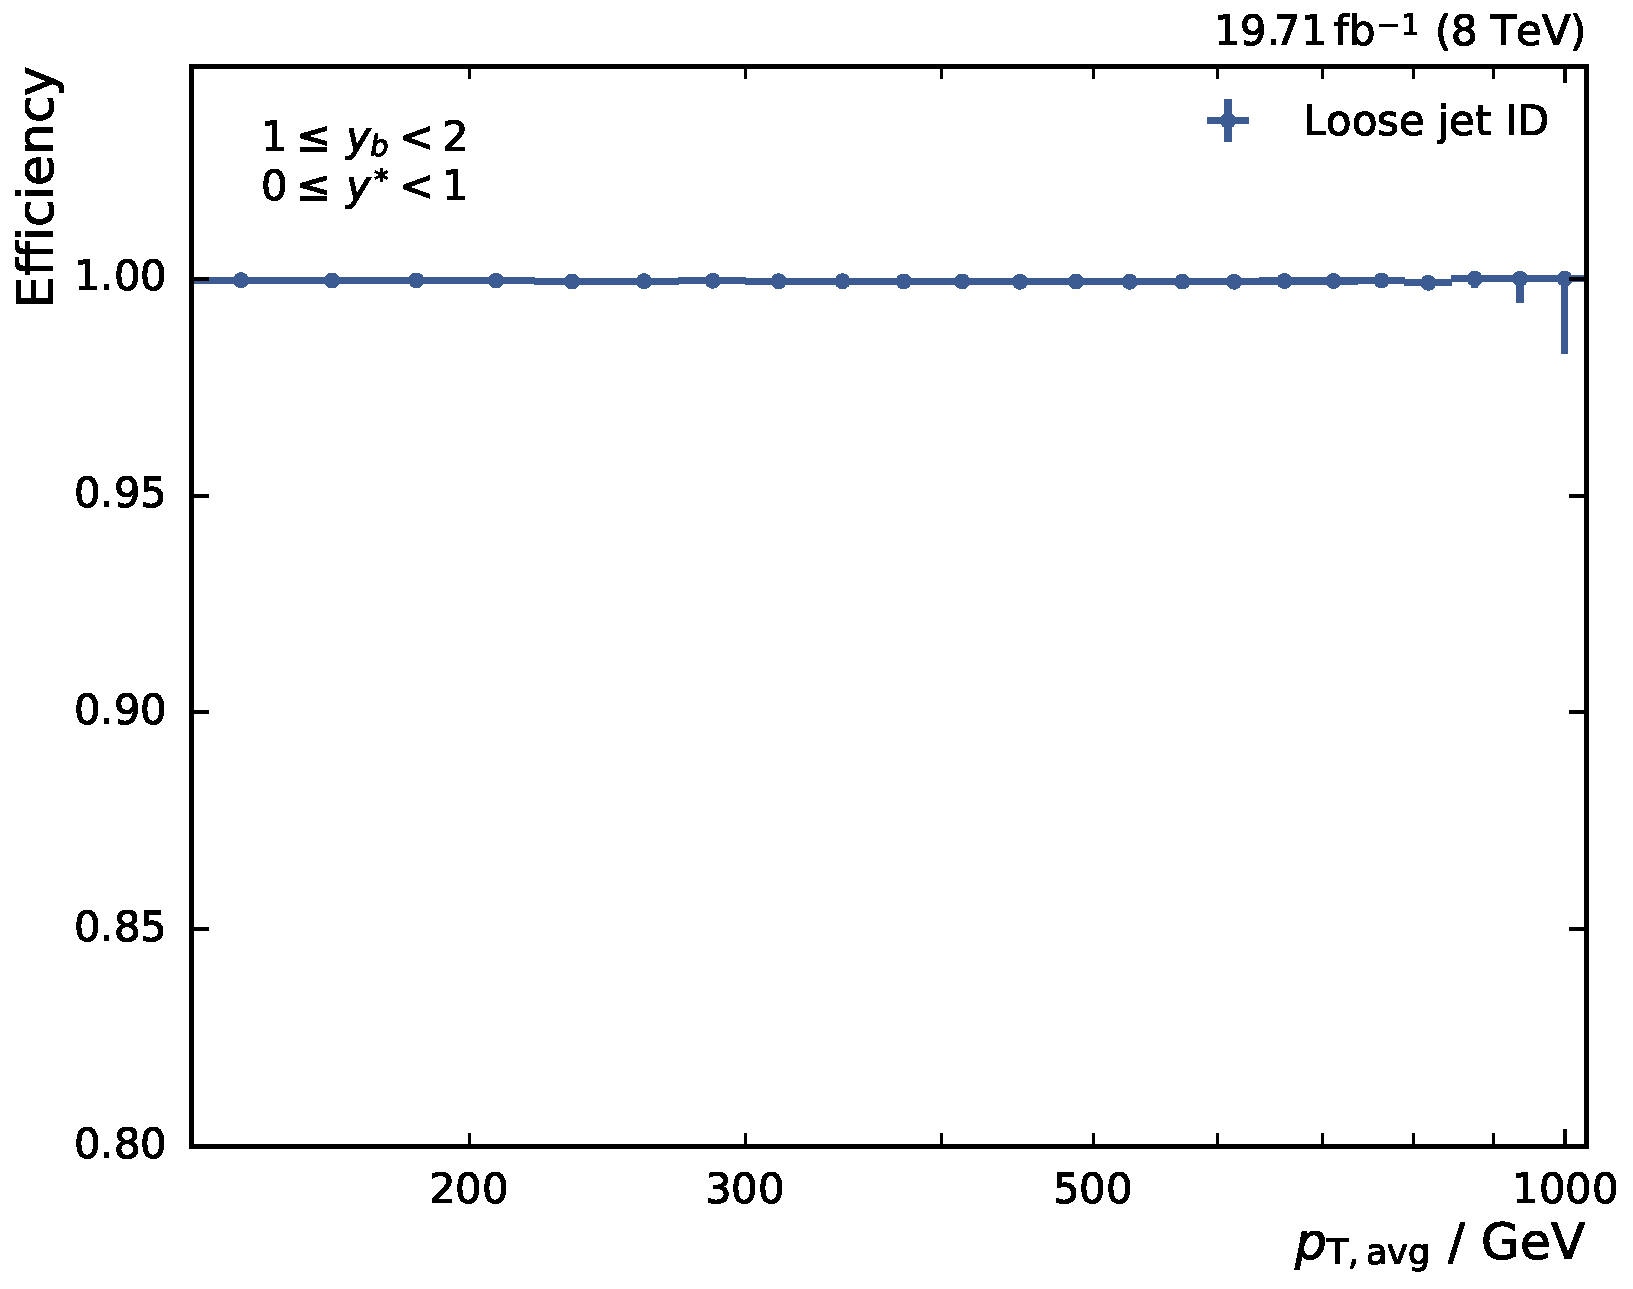
\includegraphics[width=0.49\textwidth]{figures/measurement/jetideff_yb1ys0.pdf}
    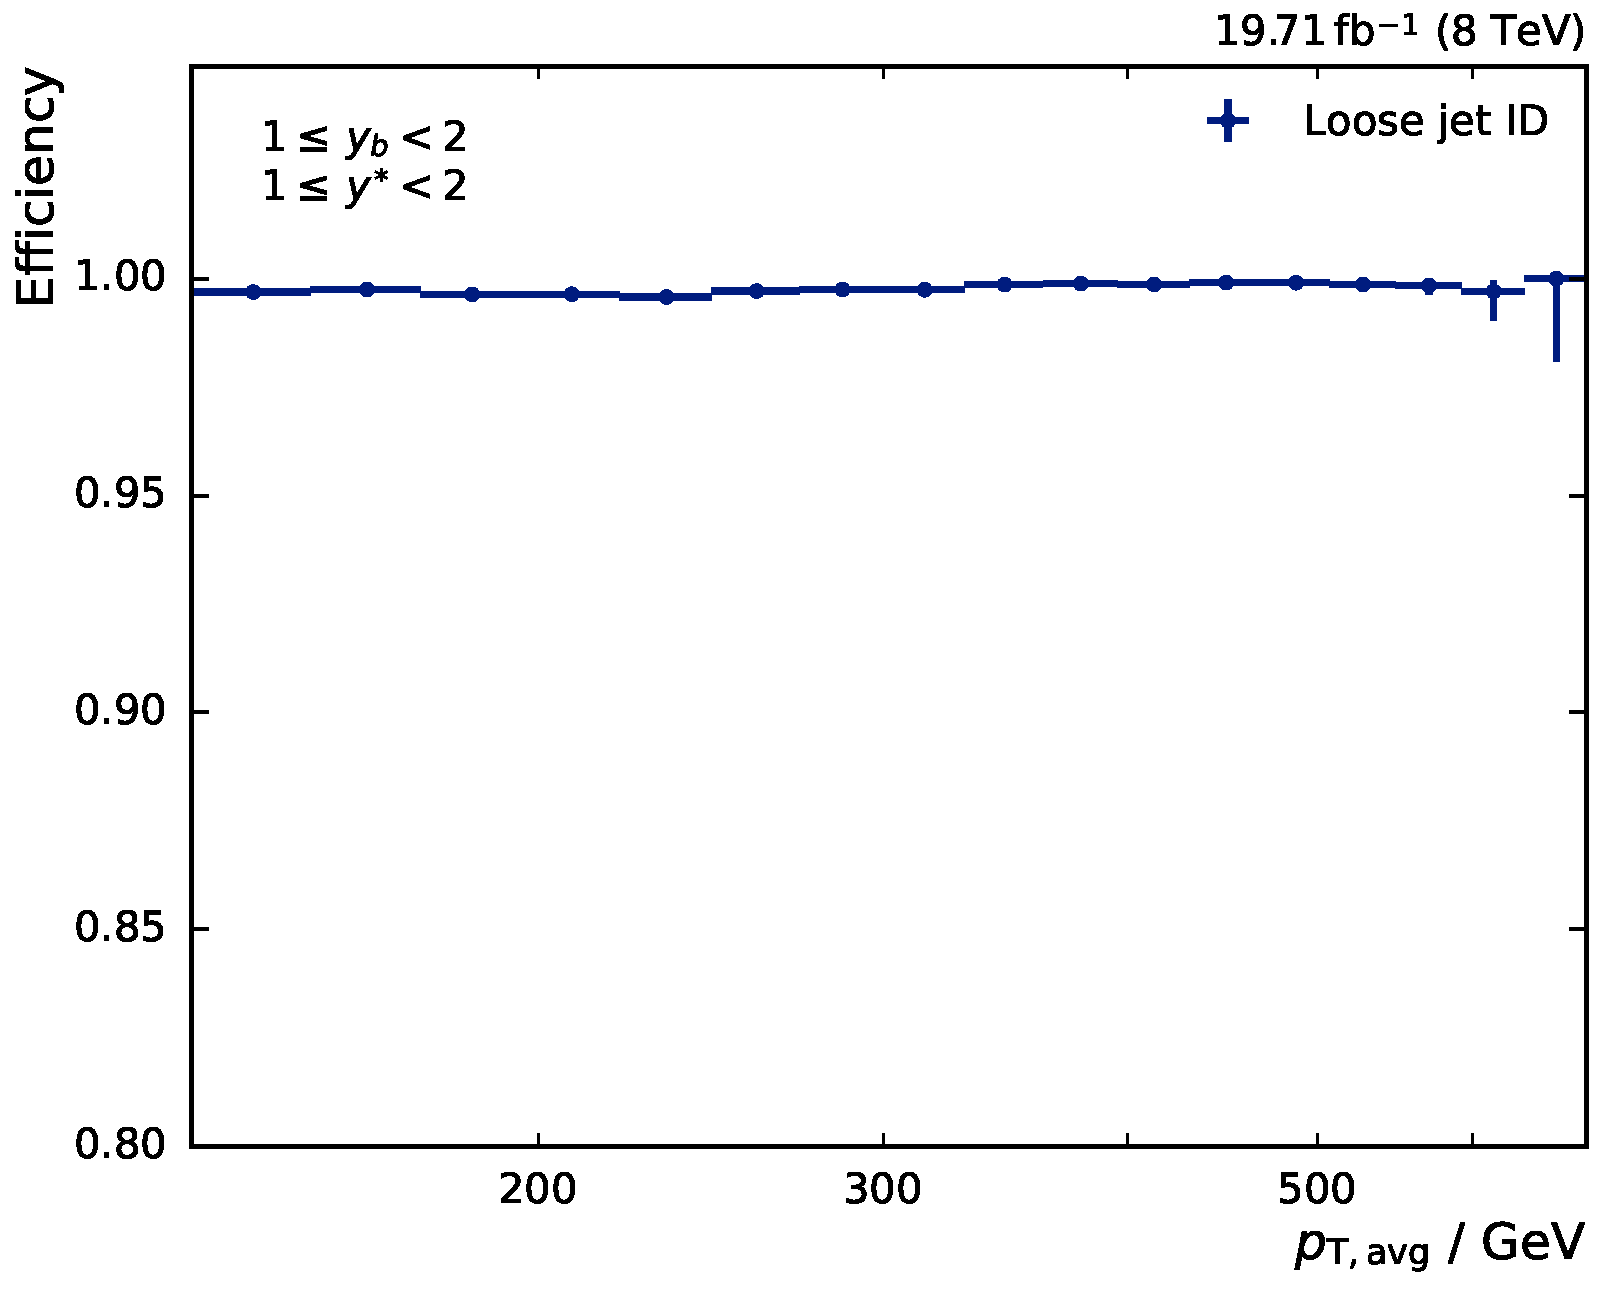
\includegraphics[width=0.49\textwidth]{figures/measurement/jetideff_yb1ys1.pdf}\hfill
    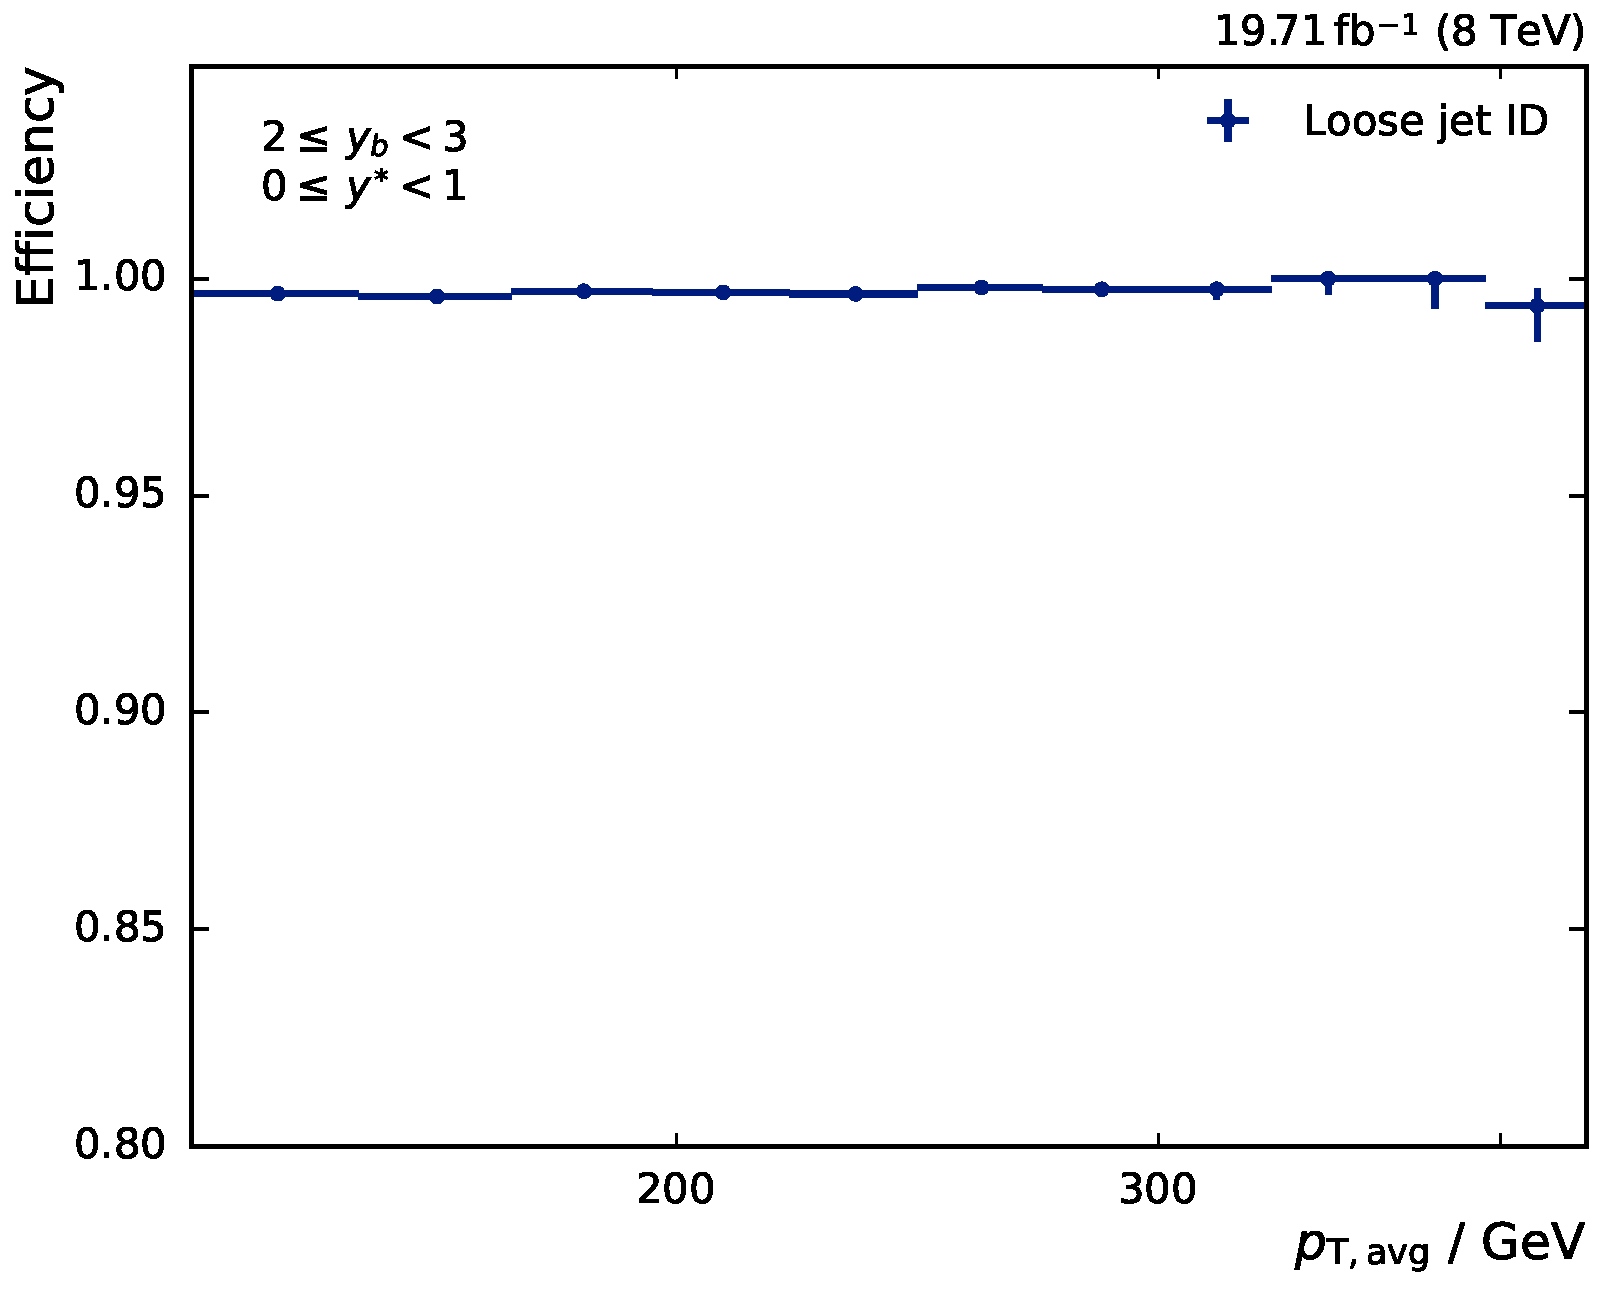
\includegraphics[width=0.49\textwidth]{figures/measurement/jetideff_yb2ys0.pdf}
    \caption[Efficiency of the jet ID]{The jet ID efficiciency as a function of
    \ptavg for all \ystar and \yboost bins. It is studied using a
    tag-and-probe approach on clean dijet event topologies. The efficiency is
    shown as a function of \ptavg for all bins. It is in all cases larger than 99\%.}
    \label{fig:jetid_eff}
\end{figure}

\subsection{Jet Correction and Selection}

This measurement is based on jets clustered from PF candidates using the
anti-\kt algorithm with a jet size parameter of 0.7. The following phase space
cuts remove jets instead of whole events due to their transverse momentum and rapidity. Consequently,
all jet energy corrections recommended by CMS are applied prior to this
selection in order to have the correct energy scale of the jets. The factorized
correction approach employed by CMS is discussed in Sec.~\ref{sec:jec} and
comprise different correction levels for jets in data\footnote{The JEC version
 applied on data is internally referred to as \texttt{Winter14\_V8}} and for
    jets in simulated events\footnote{The latest JEC for run-independent Monte
        Carlo Samples are called \texttt{START53\_V27}}.


The accessible phase space in theoretical calculations and in the measurement is
synchronized by selecting jets only from a restricted part of the complete phase
space in which the detector acceptance is high and the applicability of NLO
pQCD calculations is guaranteed.
%
\begin{align*}
    \ptjet &> \SI{50}{\GeV}\\
    |y_\mathrm{jet}| &\leq 3.0\\
\end{align*}
%
Events, in which the leading or second jet is failing the jet selection, are
discarded to only keep events in which both leading jets actually stem
from the hard scattering. Furthermore, an additional cut on the
average transverse momentum of the dijets is applied. This cut is neccessary, as
the first jet trigger becomes efficient at this point and theory calculations
and measurement have to be synchronized.
%
\begin{align*}
    \ptavg &> \SI{133}{\GeV}
\end{align*}
%
Often, it is recommended to have asymmetric cuts on the transverse momentum of
the two leading jets to avoid an infrared sensitive region. This is not an issue
here because of the much higher cut on the average transverse momentum. Other
advantage of the high cut on \ptavg are the avoidance of a turn-on region which
would lead to complications in the applied unfolding procedure as well as the
restriction to a phase space region in which non-perturbative contributions are
small.

\subsection{Jet Angular Correction}

The jet energy corrections relate the reconstructed jet energy to the
particle level jet energy, but they do not include any correction for angular
reconstruction deficiencies of the jets. However, especially in the transition
regions of the detector, \ie when the tracker coverage ends, a systematic
reconstruction bias is observed, see Fig.~\ref{fig:jet_eta_corr}. Jets are
reconstructed with systematically larger absolute pseudo-rapidity, \ie shifted
towards the forward region. While the absolute shift is rather small, it's a
relevant systematic effect when the rapidity separation of two jets is of
interest. However, two effects limit the impact of the mismodelling. First, it
is only pronounced for jets with low transverse momentum as can be seen in
Fig~\ref{fig:jet_eta_corr_vs_pt} and second, the large bin size in rapidity
reduces the effects. 

Nonetheless, the systematic error is accounted for by applying a correction on
each jet based on the average difference between the pseudo-rapidity of
particle level jets and reconstructed jets as a function of reconstructed jet
\pt and pseudo-rapidity. The Figs.~\ref{fig:jet_eta_corr} and
~\ref{fig:jet_eta_corr_vs_pt} also show the dstribution after applying the
correction, in which the majority of the $\eta$ dependent effects is removed.

\begin{figure}[htbp]
    \centering
    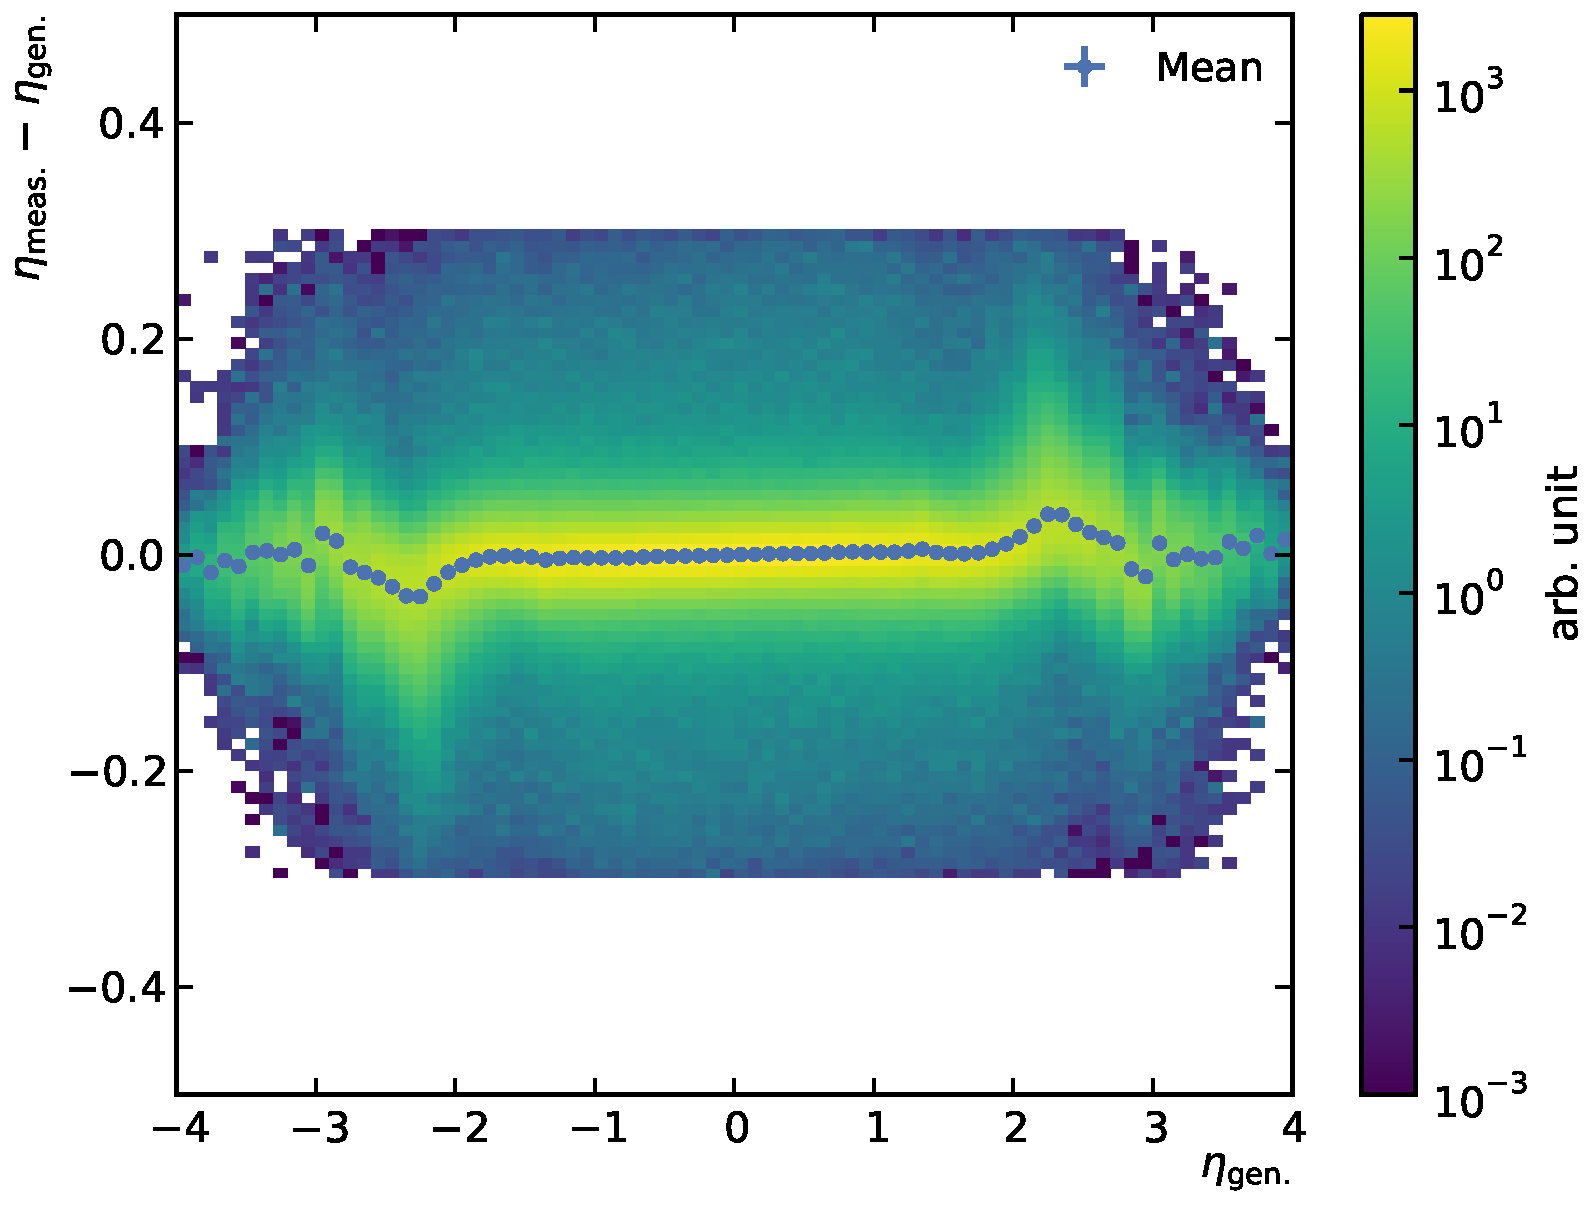
\includegraphics[width=0.49\textwidth]{figures/measurement/genvsreco_eta.pdf}\hfill
    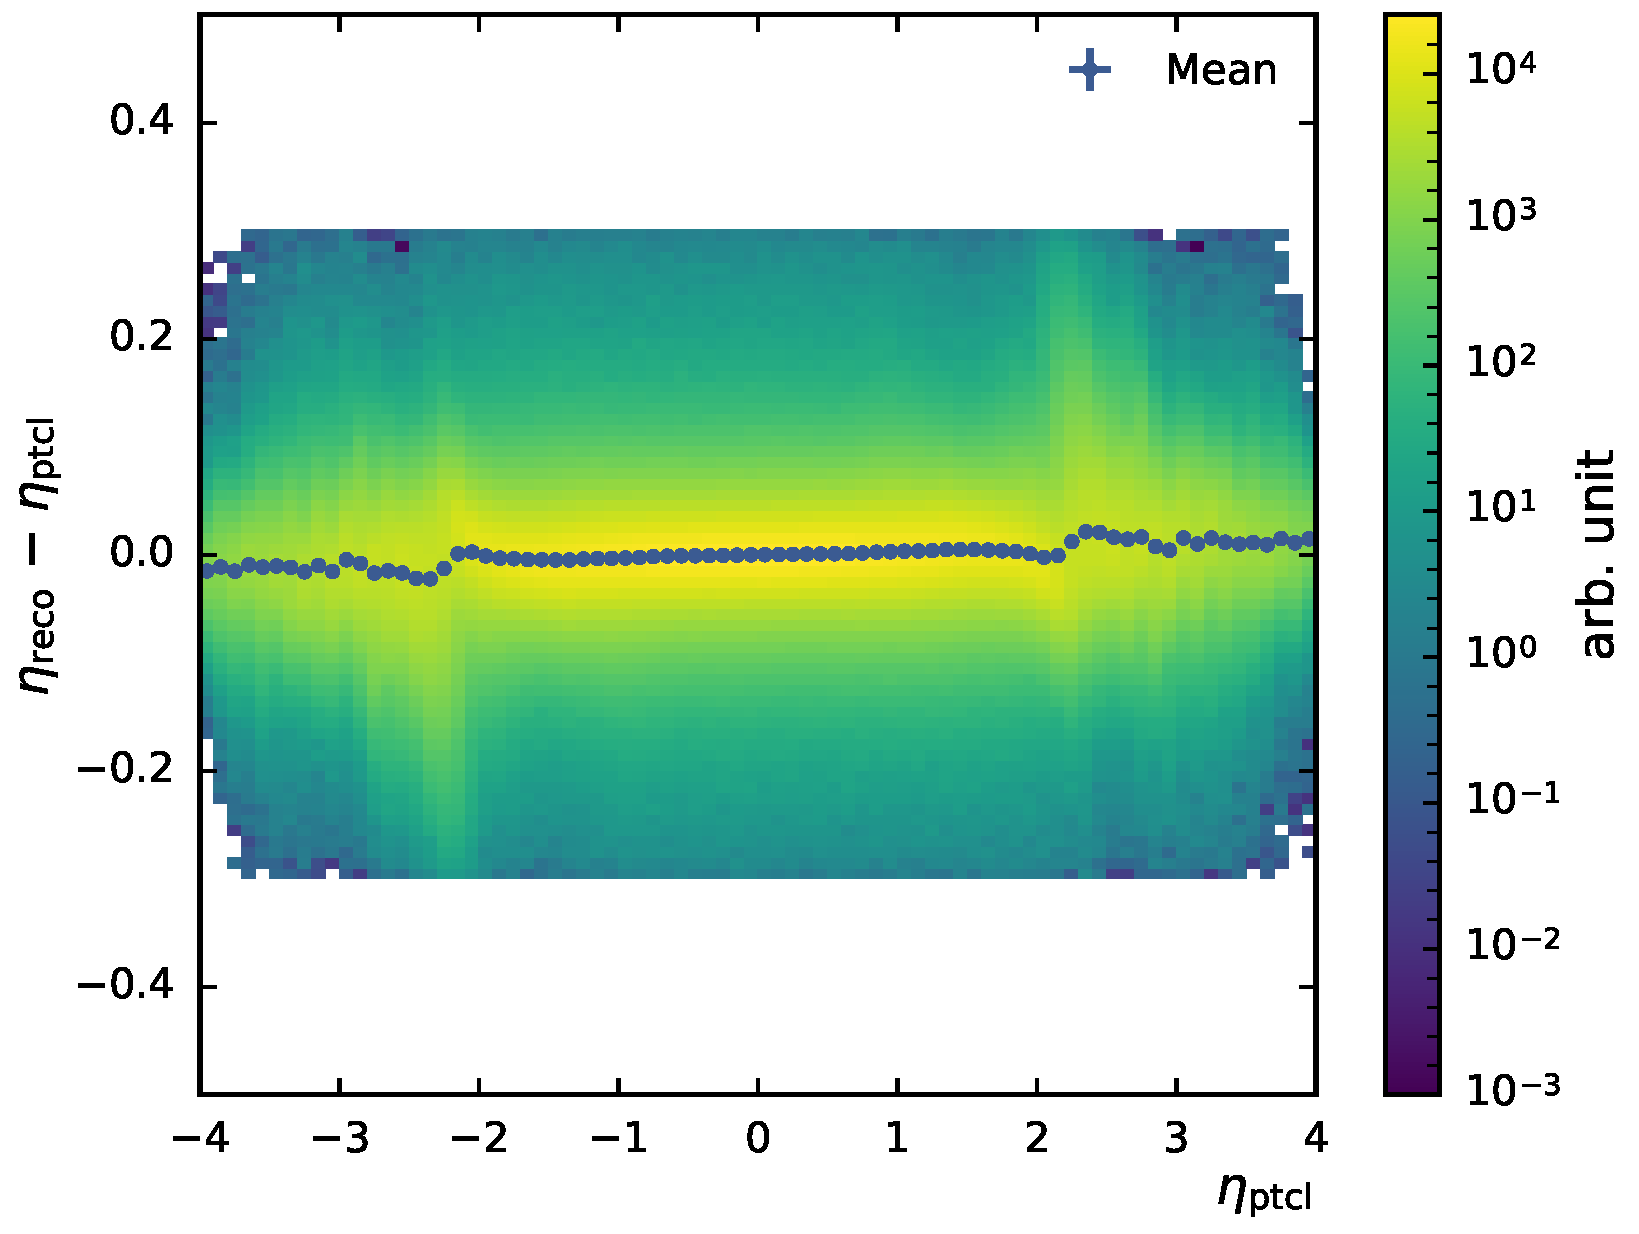
\includegraphics[width=0.49\textwidth]{figures/measurement/genvsreco_eta_corr.pdf}
    \caption[Differences of pseudo-rapidity of reconstructed jets to
        generator-level jets]{The difference between the pseudo-rapdity of the
            reconstructed jets and the generated jets is shown over the
            pseudo-rapidity of the generated jet. The distribution is shown
            before (left) and after (right) applying the pseudo-rapidity
            correction. The blue points indicate the mean of the distribution in
            each $\eta_{\mathrm{gen}}$ bin.}
    \label{fig:jet_eta_corr}
\end{figure}


\begin{figure}[htbp]
    \centering
    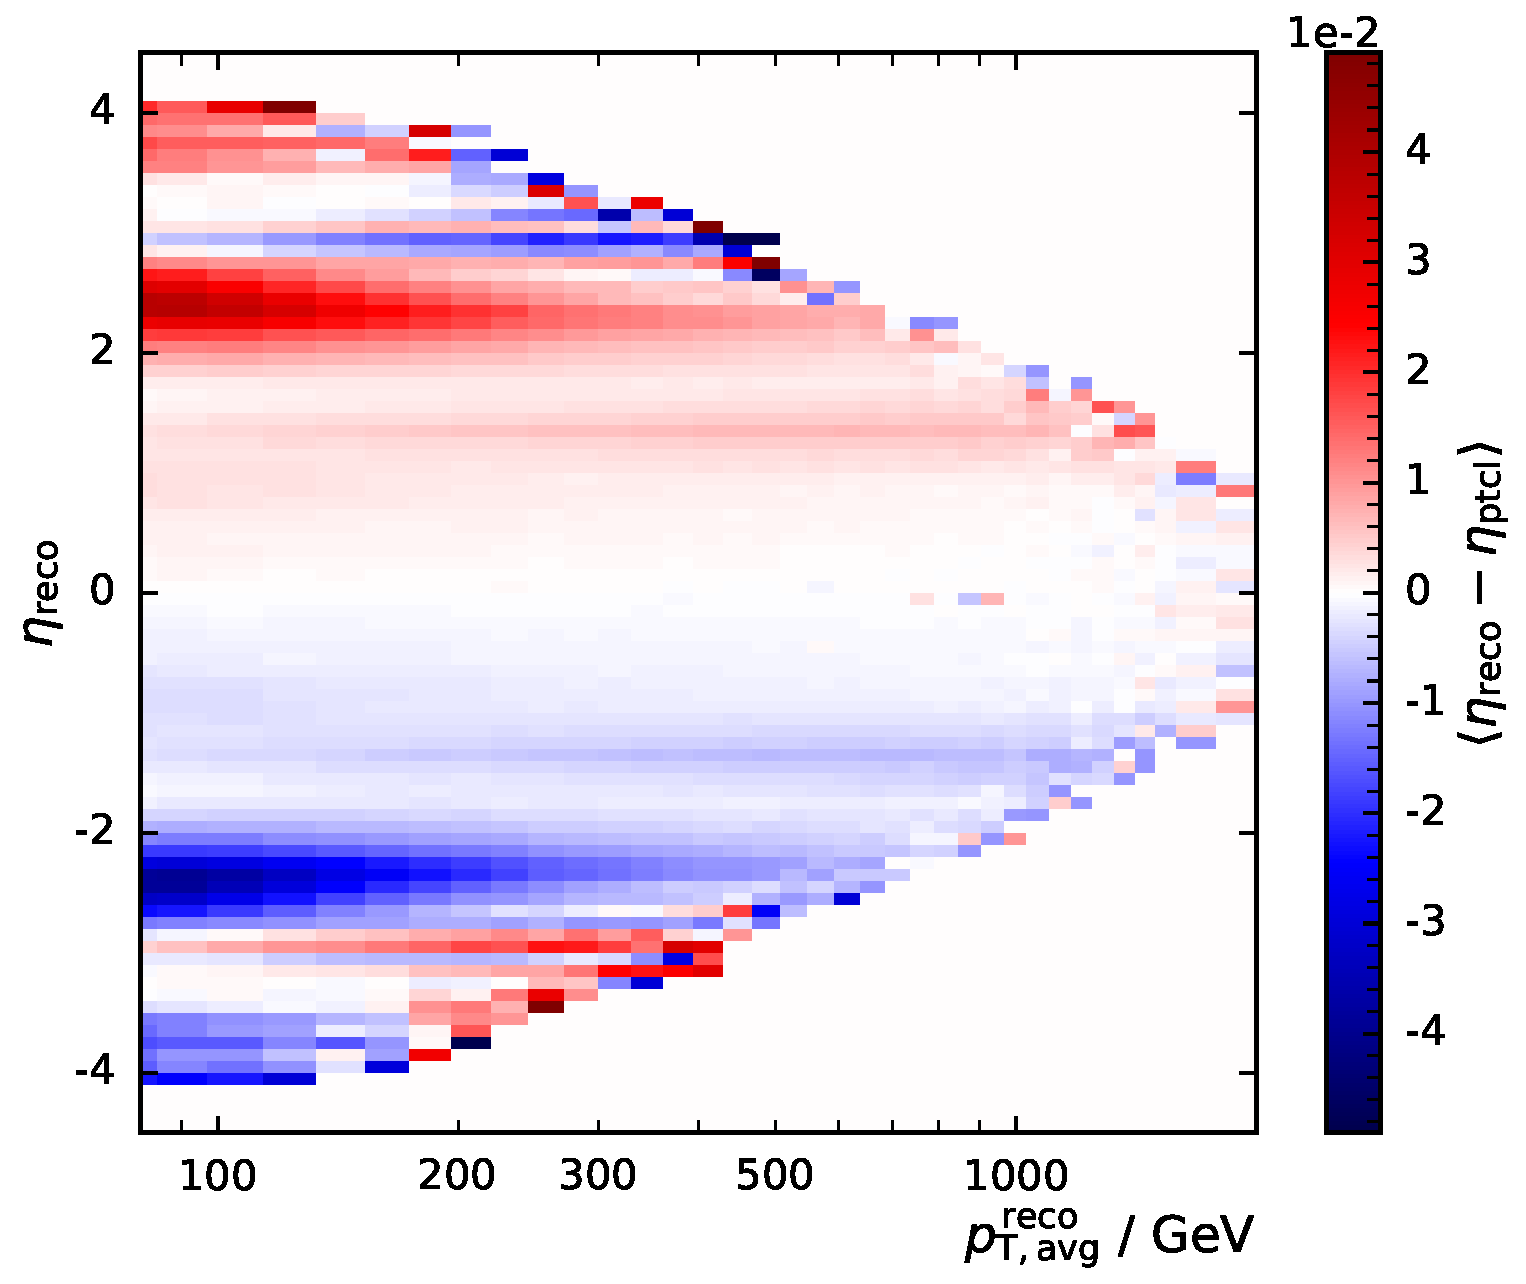
\includegraphics[width=0.49\textwidth]{figures/measurement/genvsreco_eta_vs_genpt.pdf}\hfill
    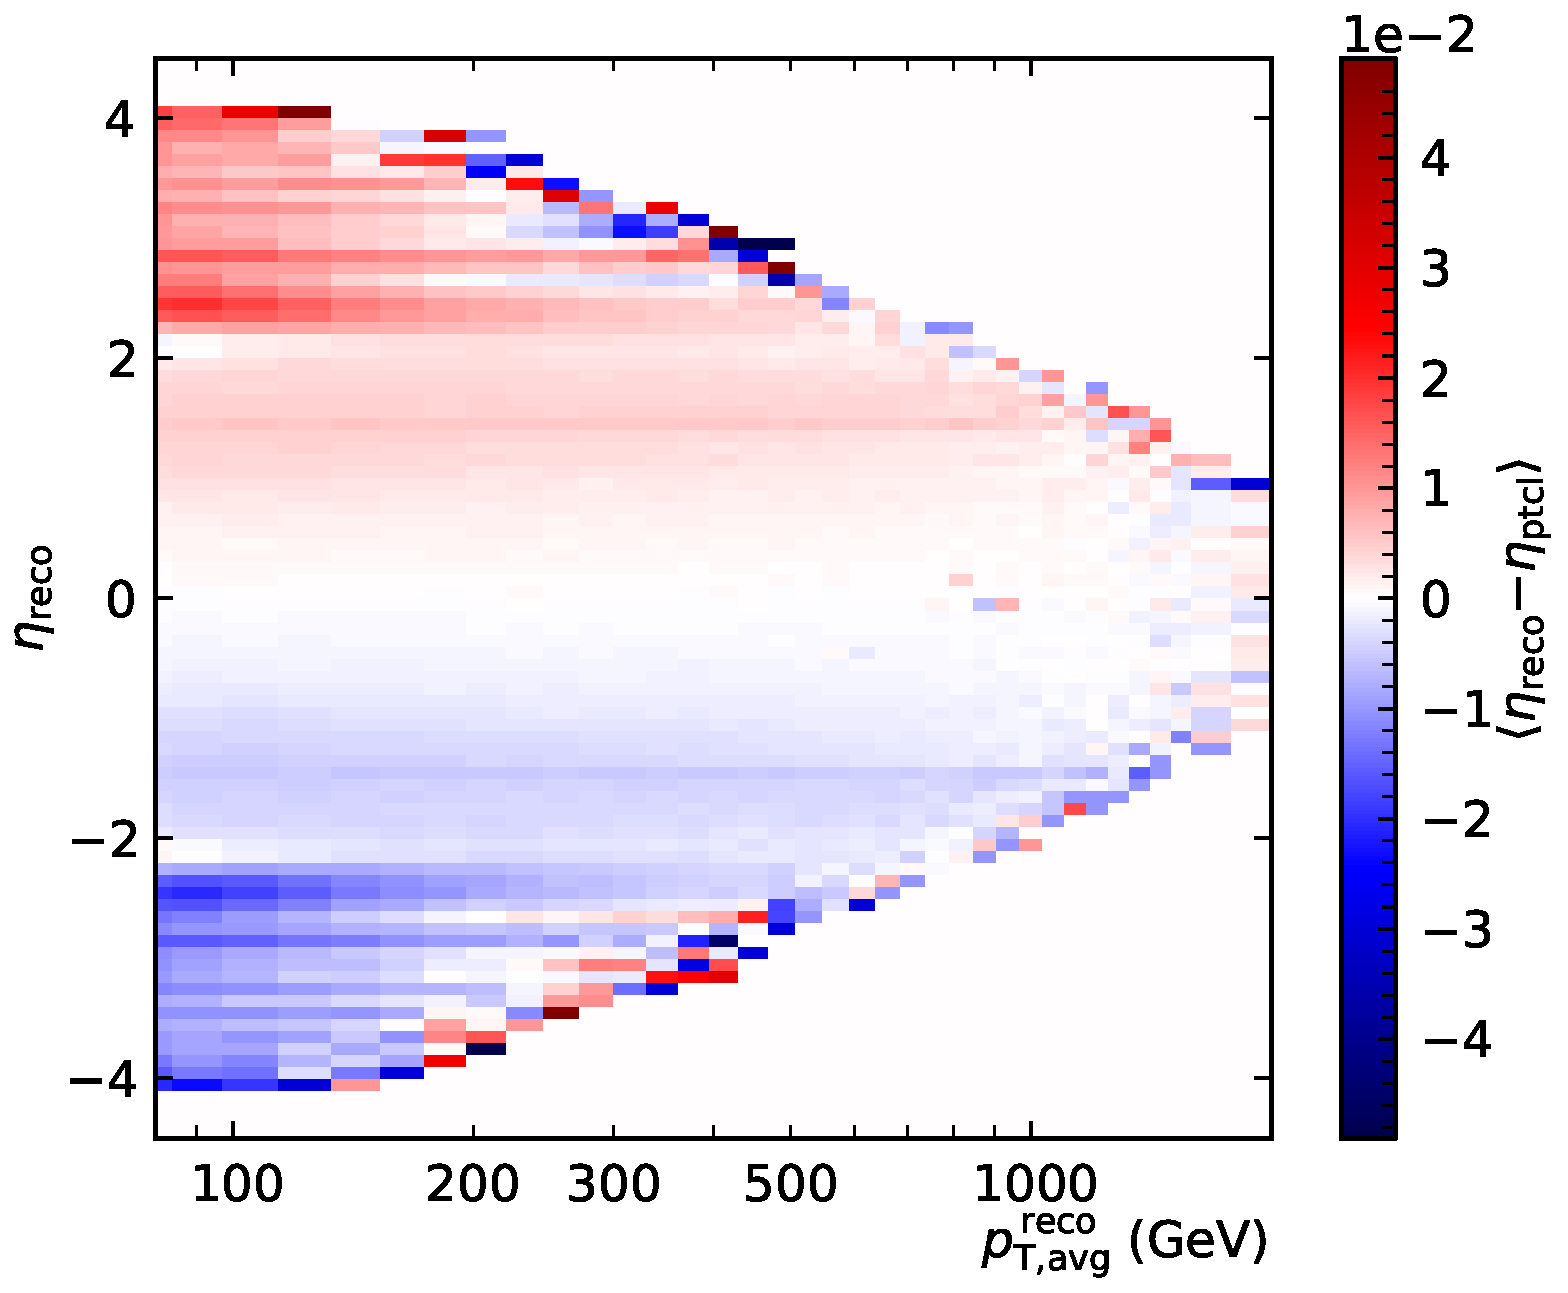
\includegraphics[width=0.49\textwidth]{figures/measurement/genvsreco_eta_vs_genpt_corr.pdf}
    \caption[Differences of pseudo-rapidity of reconstructed jets and particle level jets as a function of the reconstructed jet \pt]
            {The pseudo-rapidity of the
            generated jets is shown as a function of the transverse momentum of
            the jets. The color indicates the differences of the pseudo-rapidity
            of the generated and reconstructed jets. The distribution is shown
            before (left) and after (right) the angular
        correction is applied.}
    \label{fig:jet_eta_corr_vs_pt}
\end{figure}

To estimate the effect on the resulting cross section, a comparison between the
yielded cross section with and without applying the pseudo-rapidity correction
is given in Fig.~\ref{fig:rap_corr_data}. As can be seen immediately, the effect is
rather small. In the measurement bins containing forward jets, the correction
causes about 2\% changes of the cross section. Since these events move to bins
containing more central jets and therefore have a much higher cross section, the
cross section increase is not noticeably.

\begin{figure}[htbp]
    \centering
    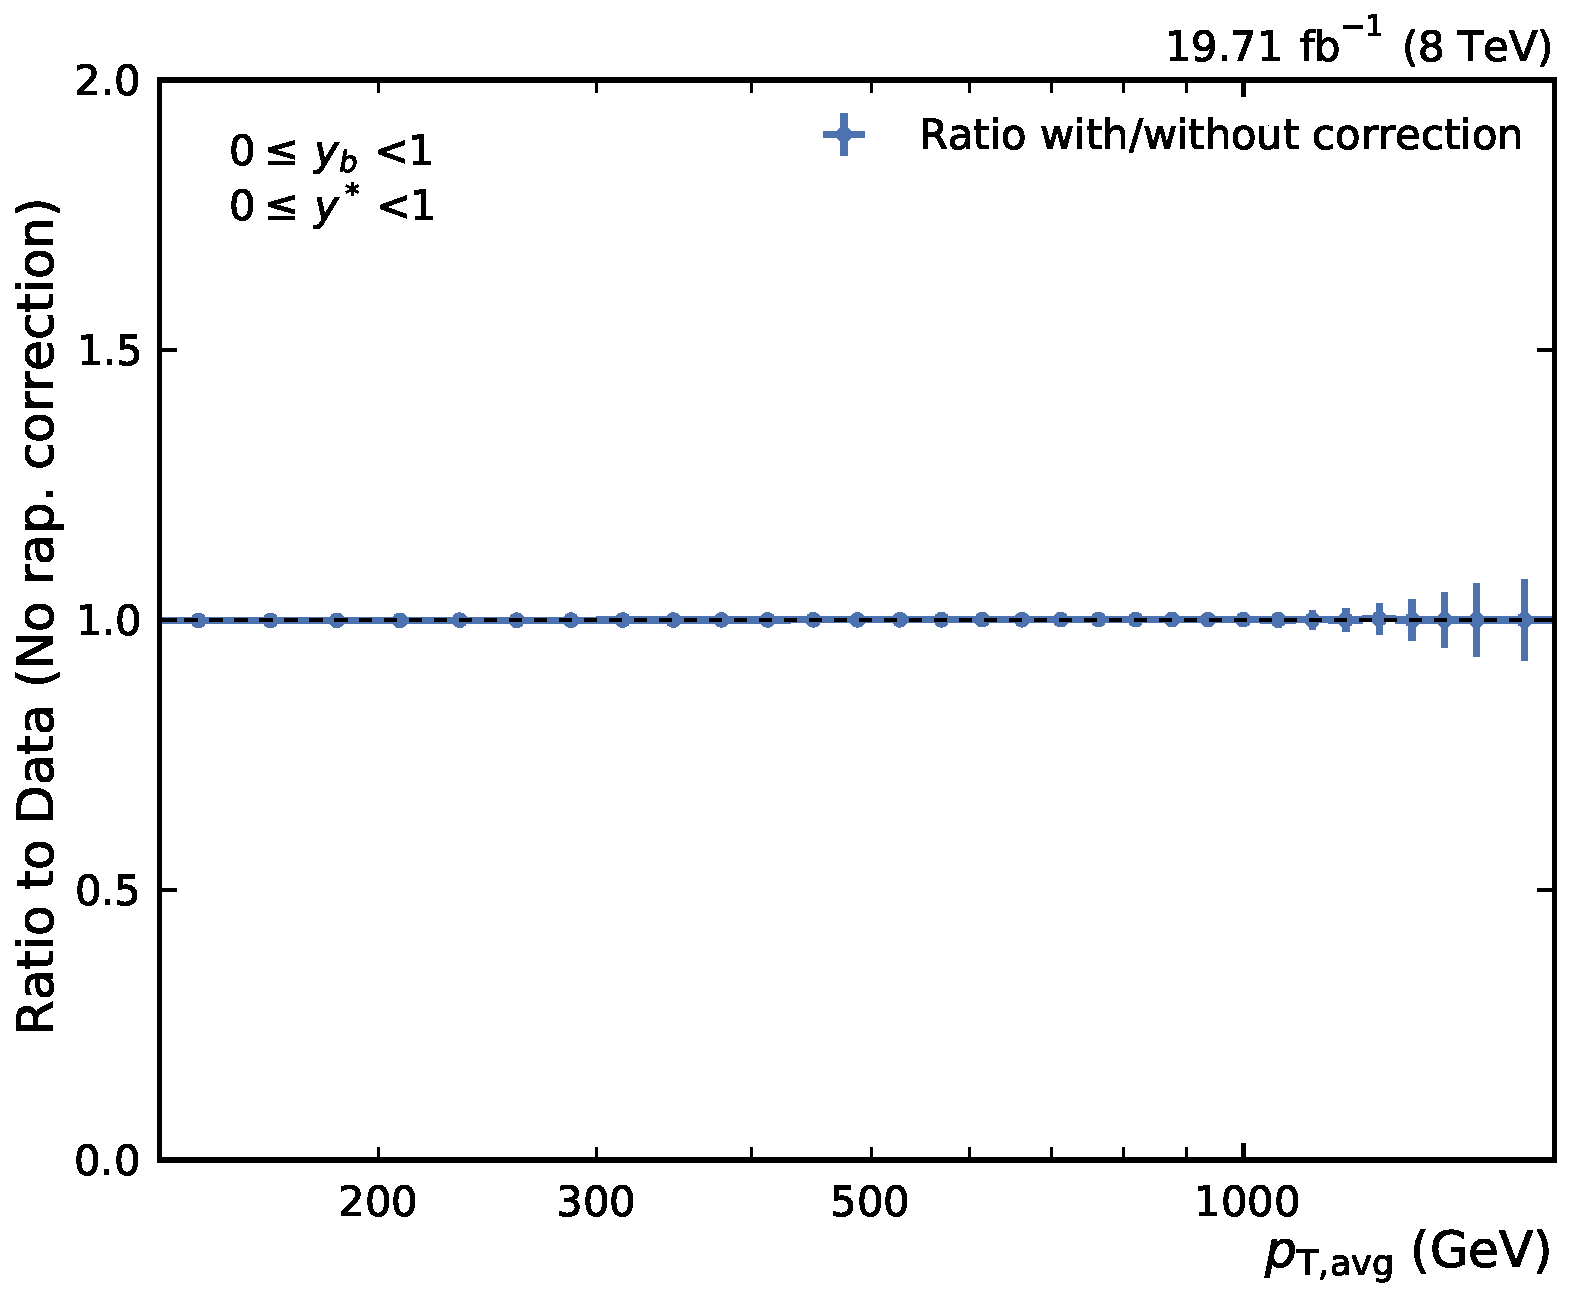
\includegraphics[width=0.47\textwidth]{figures/measurement/rap_corr_data_yb0ys0.pdf}\hfill
    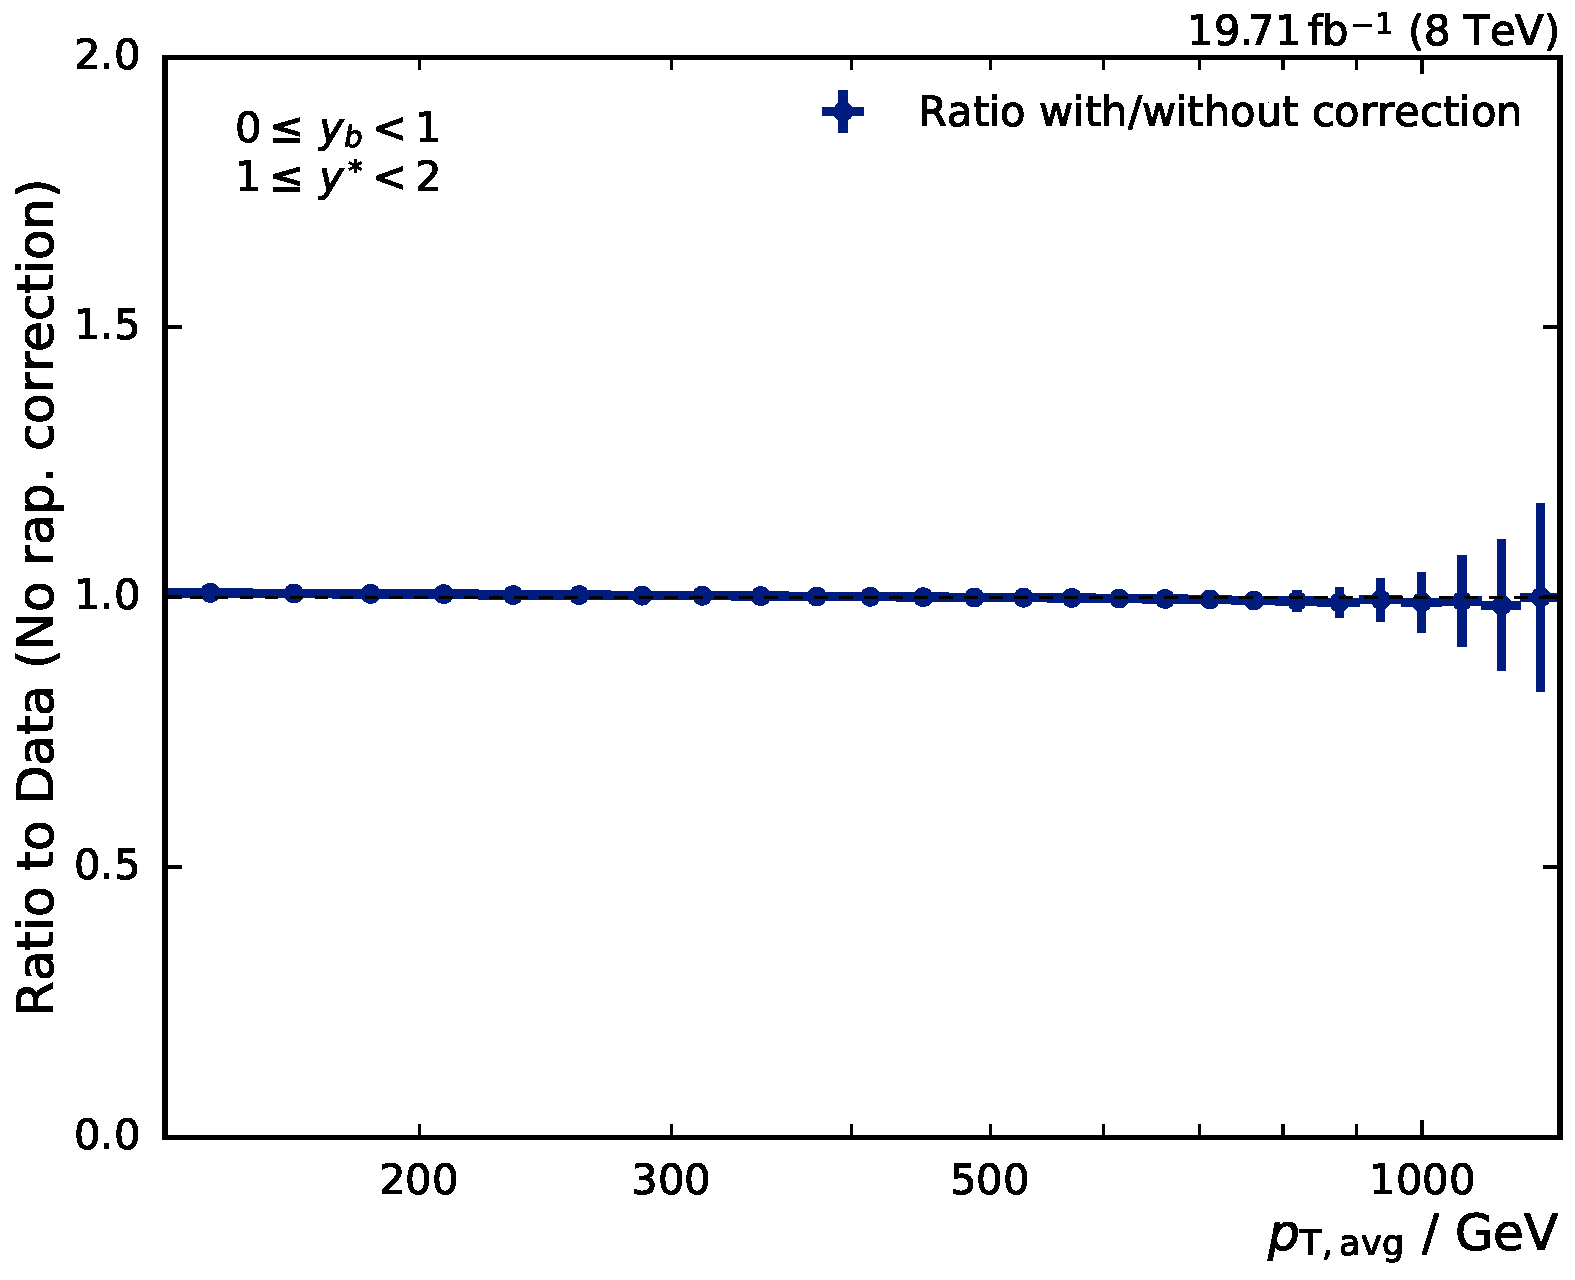
\includegraphics[width=0.47\textwidth]{figures/measurement/rap_corr_data_yb0ys1.pdf}
    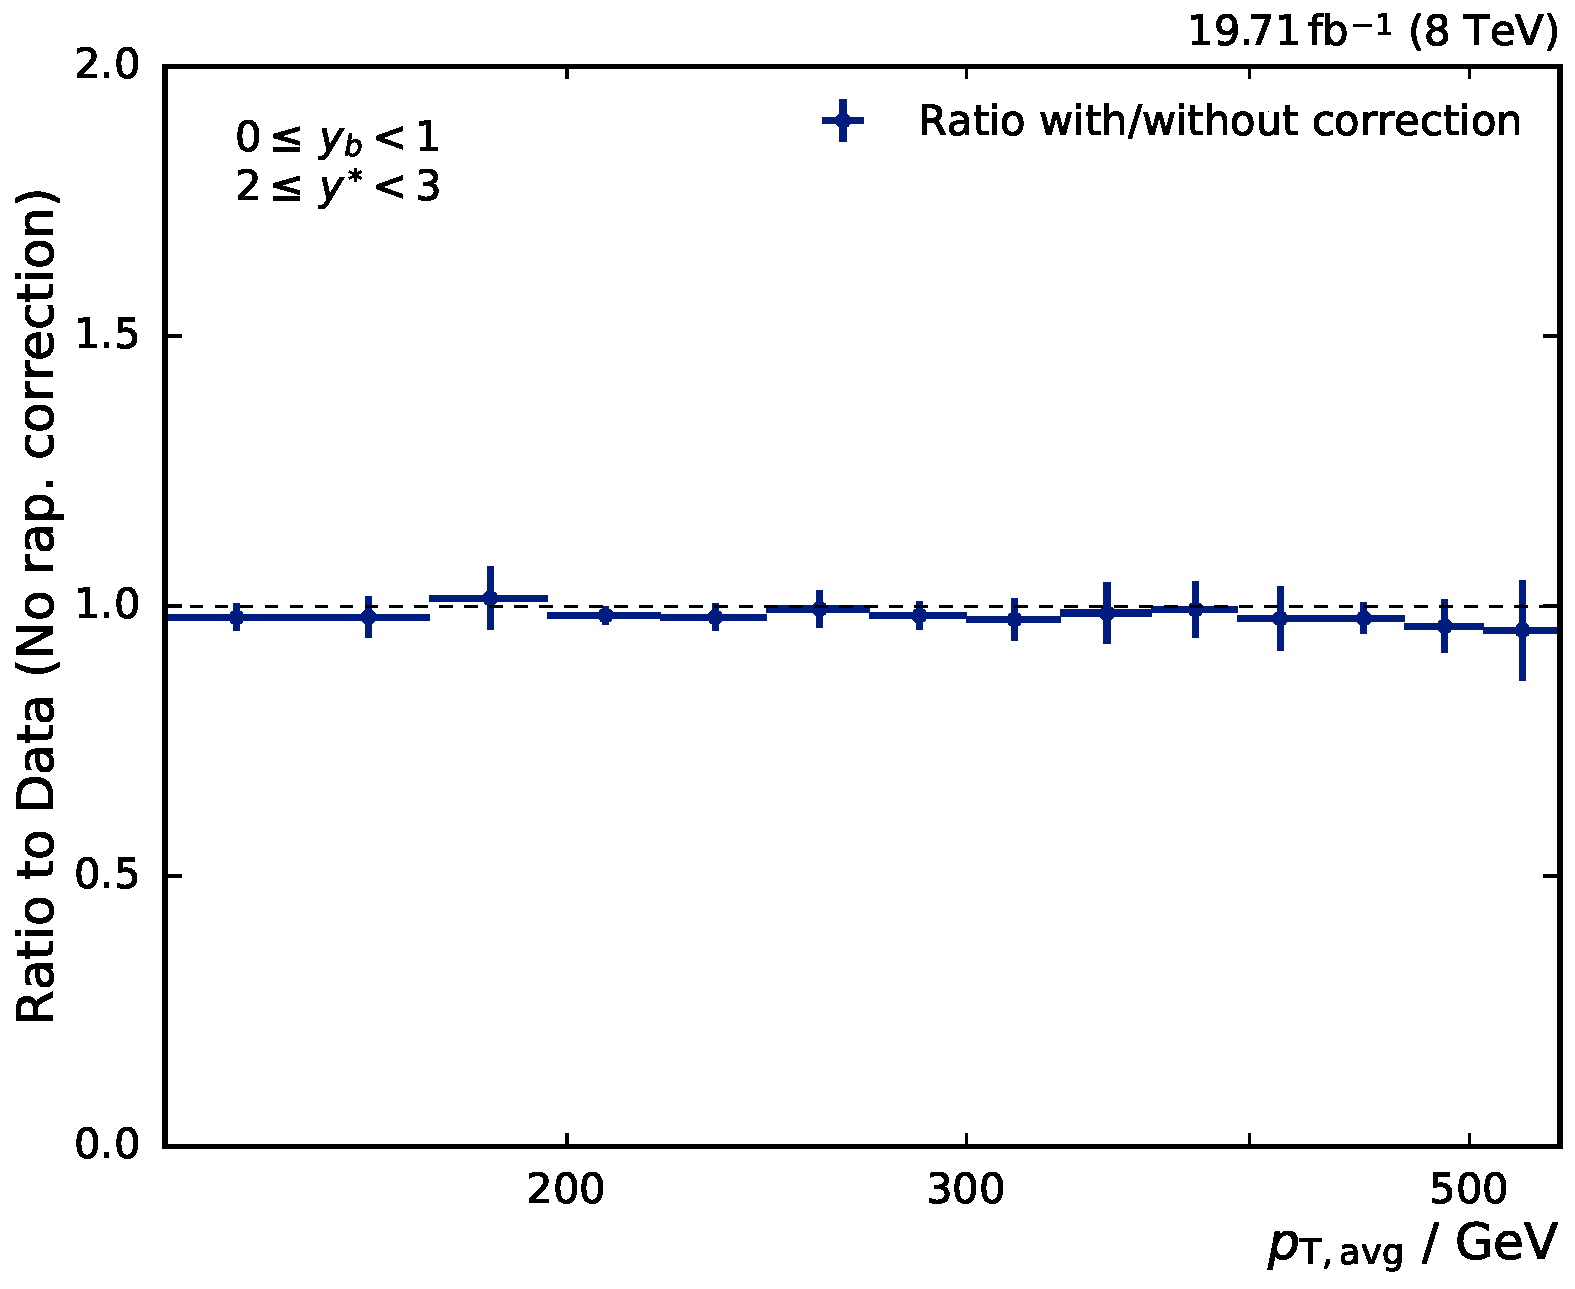
\includegraphics[width=0.47\textwidth]{figures/measurement/rap_corr_data_yb0ys2.pdf}\hfill
    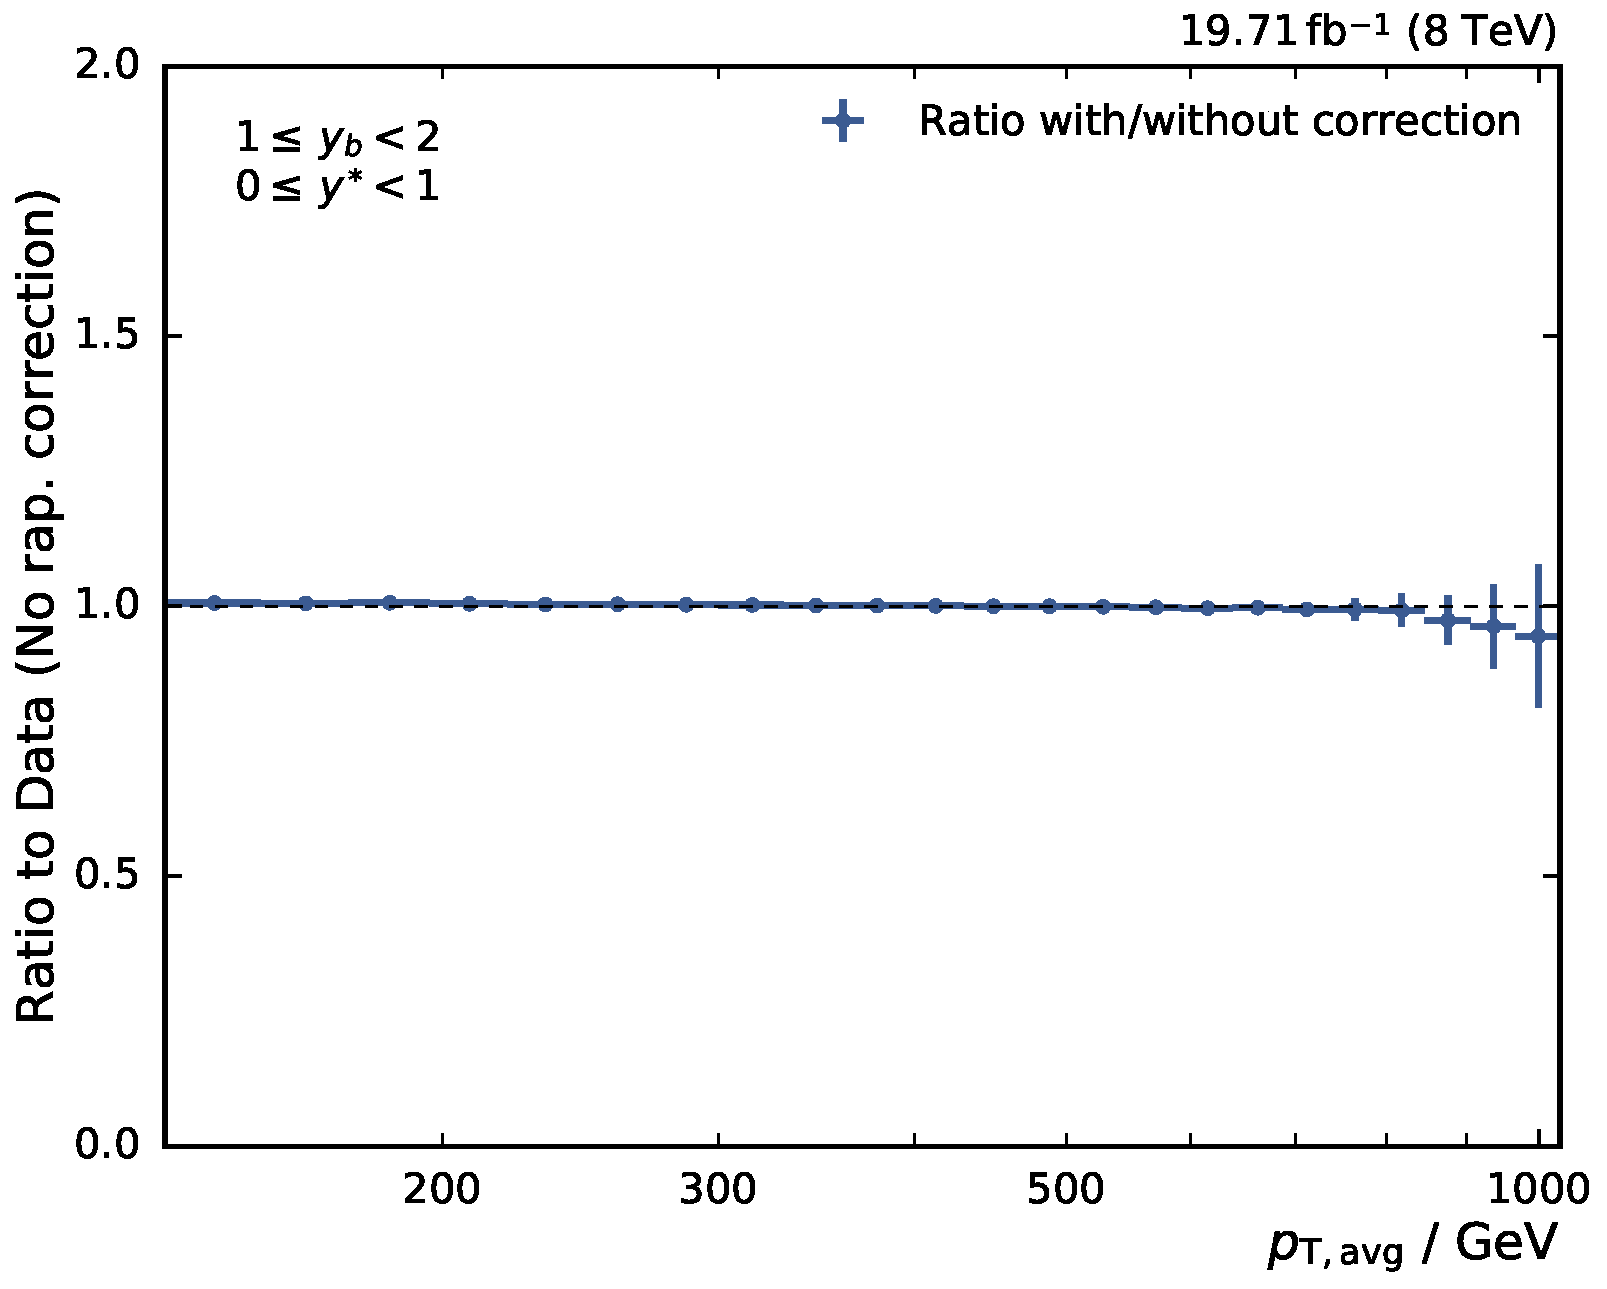
\includegraphics[width=0.47\textwidth]{figures/measurement/rap_corr_data_yb1ys0.pdf}
    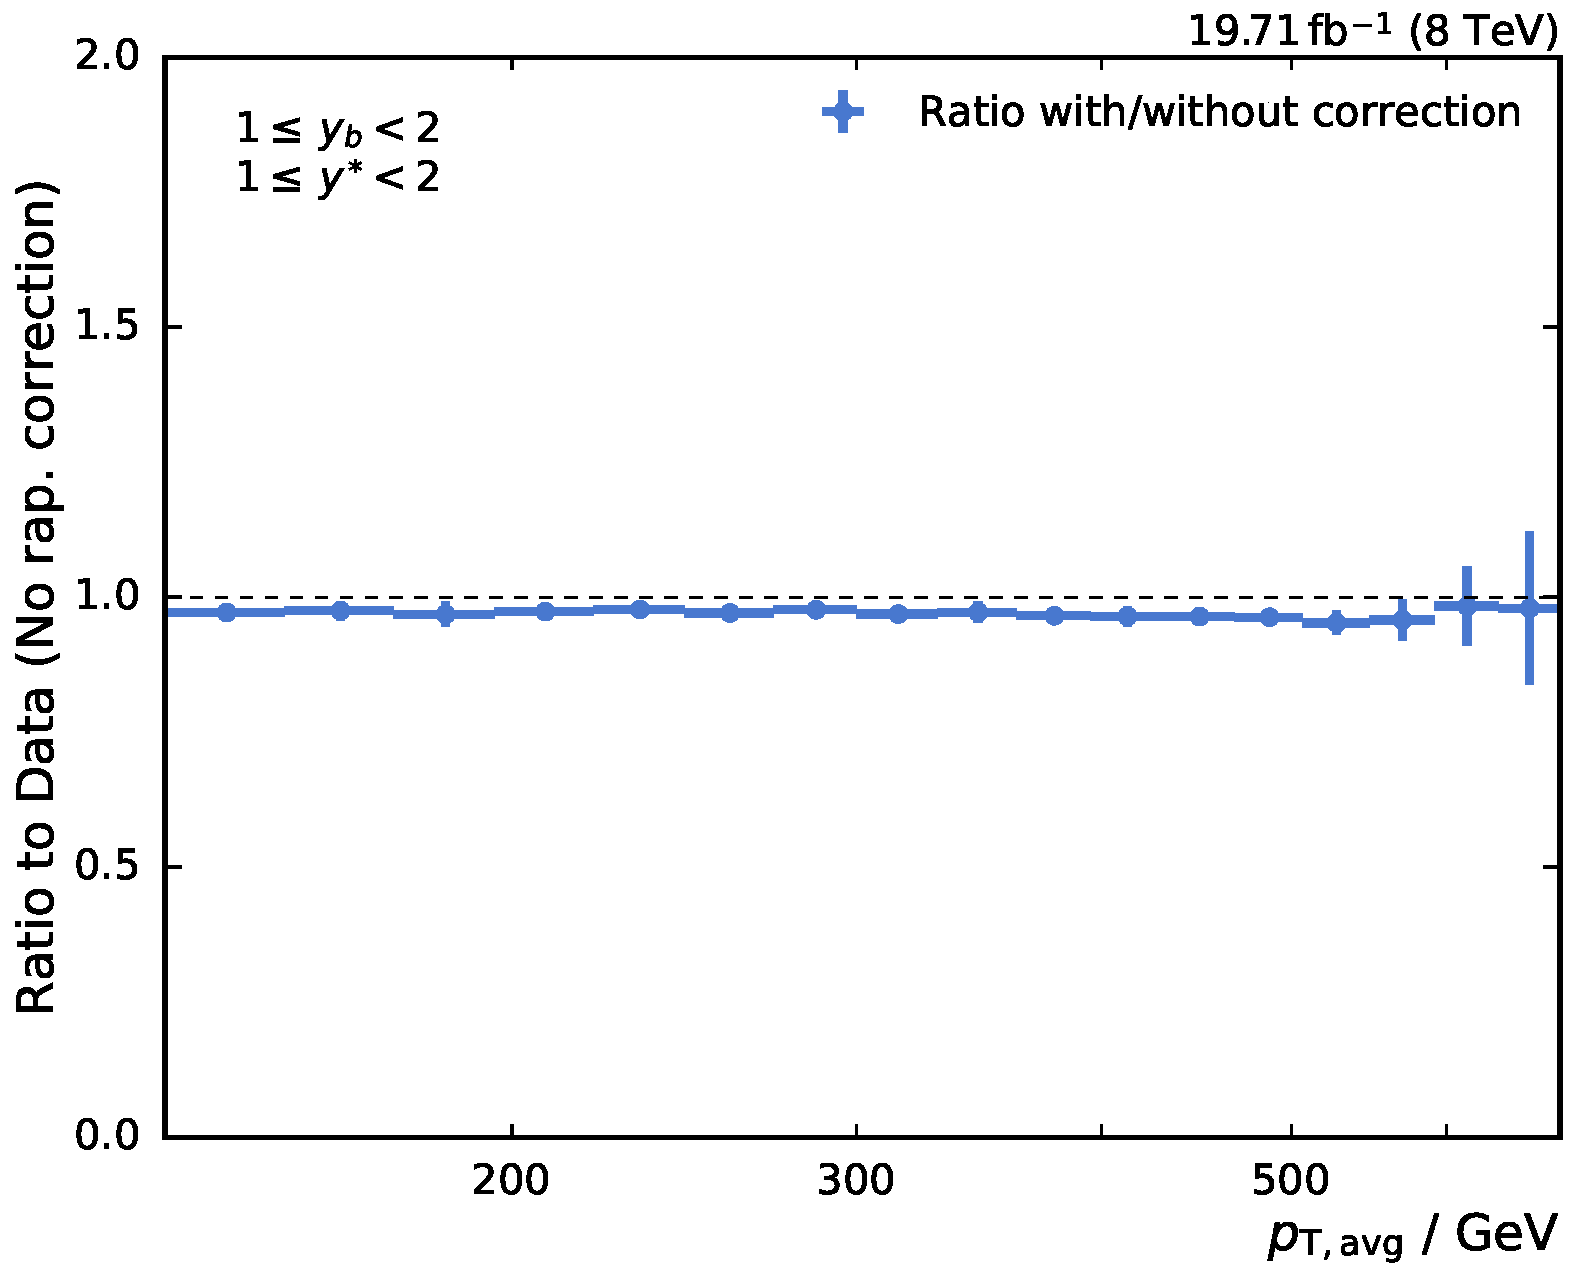
\includegraphics[width=0.47\textwidth]{figures/measurement/rap_corr_data_yb1ys1.pdf}\hfill
    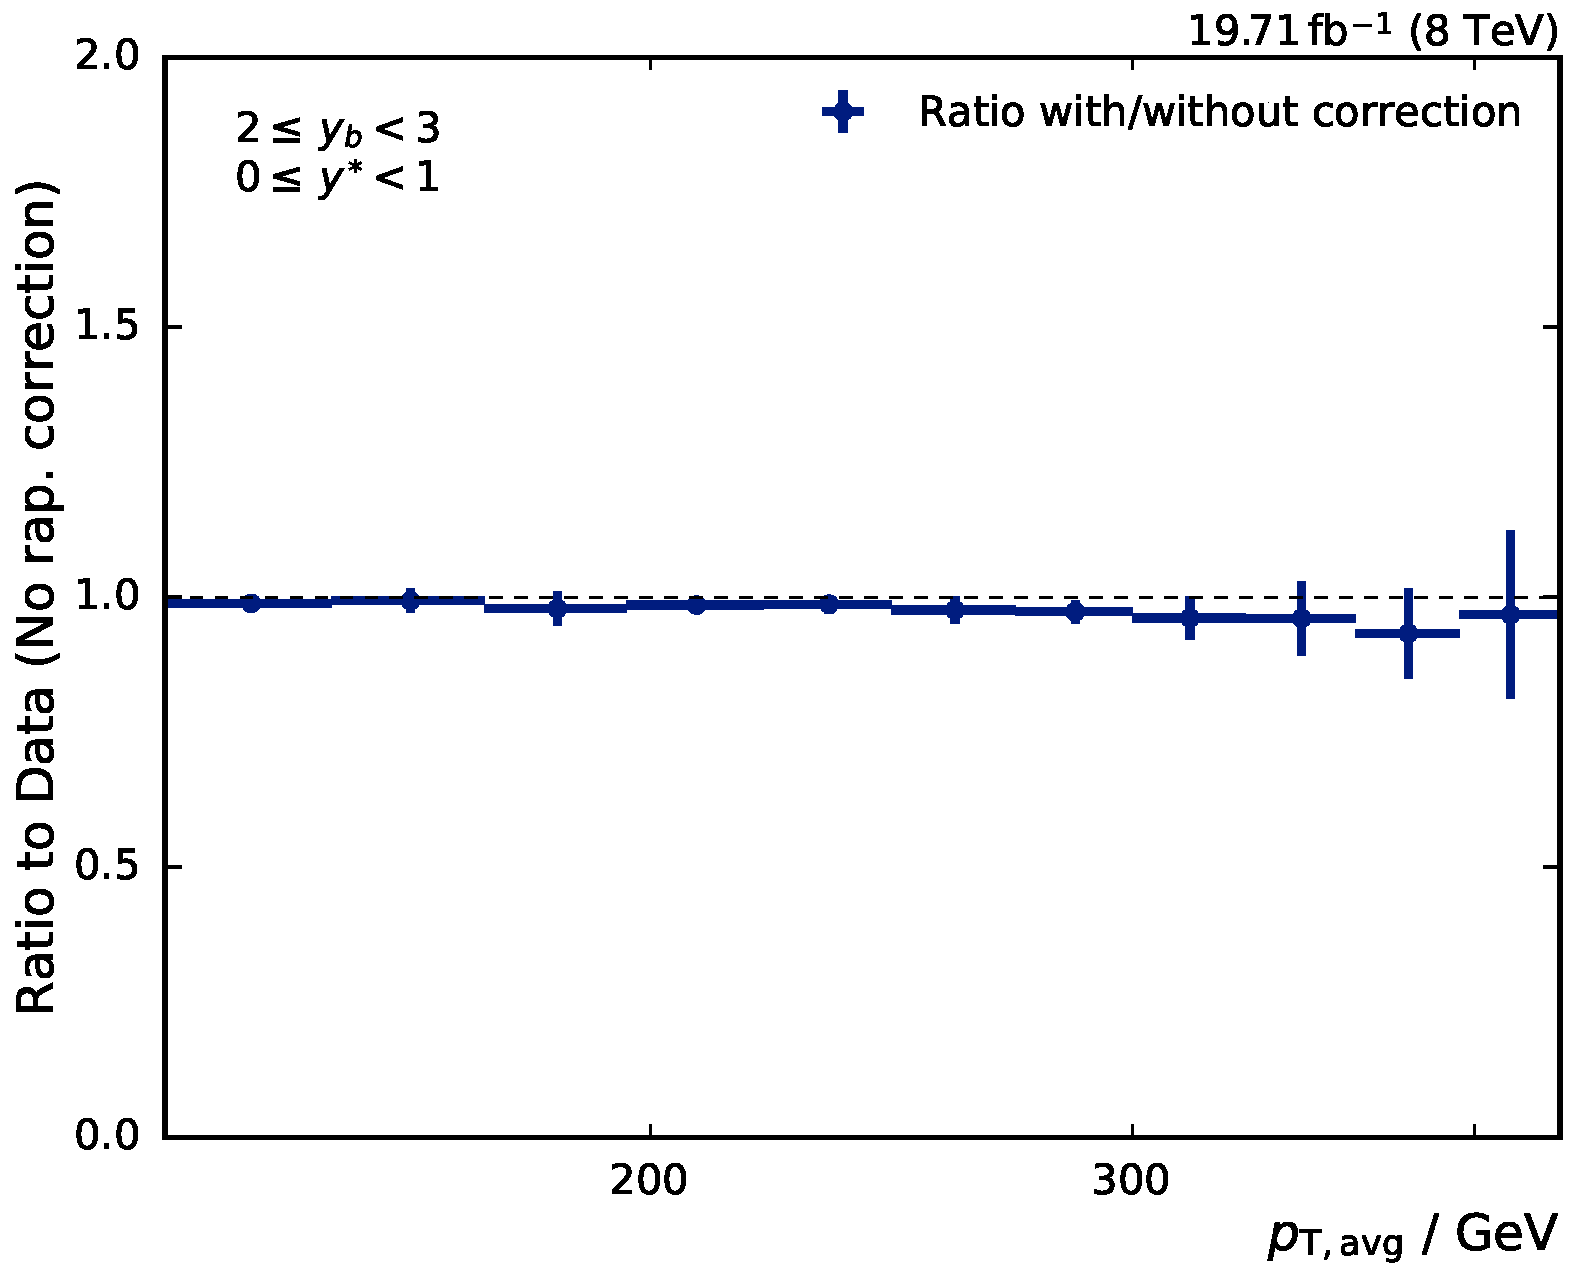
\includegraphics[width=0.47\textwidth]{figures/measurement/rap_corr_data_yb2ys0.pdf}
    \caption[Effect of angular correction]{The effect of the angular correction
        on the cross section  is demonstrated by calculating the ratio of the
        cross section after applying the correction to the one without
        correction. The cross section decreases in bins involving forward jets
        and is more pronounced for higher values of \ystar.}
    \label{fig:rap_corr_data}
\end{figure}

\subsection{Stability versus Run Periods}

The experimental conditions for data-taking change slightly over the various run
periods, due to changes of the detector calibration or different trigger
prescales. Nonetheless the finally measured cross section must not depend on
these effects. This is checked by calculating the result separately for each run
period, see Fig.~\ref{fig:run_comparison}, which shows the ratio of the cross
section in each run period to the cross section obtained in run D. 

There are changes visible, most notably due to statistical fluctuations in the
high-\pt region. Futhermore, a slight slope of the cross section obtained in run
B is observed. However, in general all results are in good agreement and the
differences are negligible.

\begin{figure}[htbp]
    \centering
    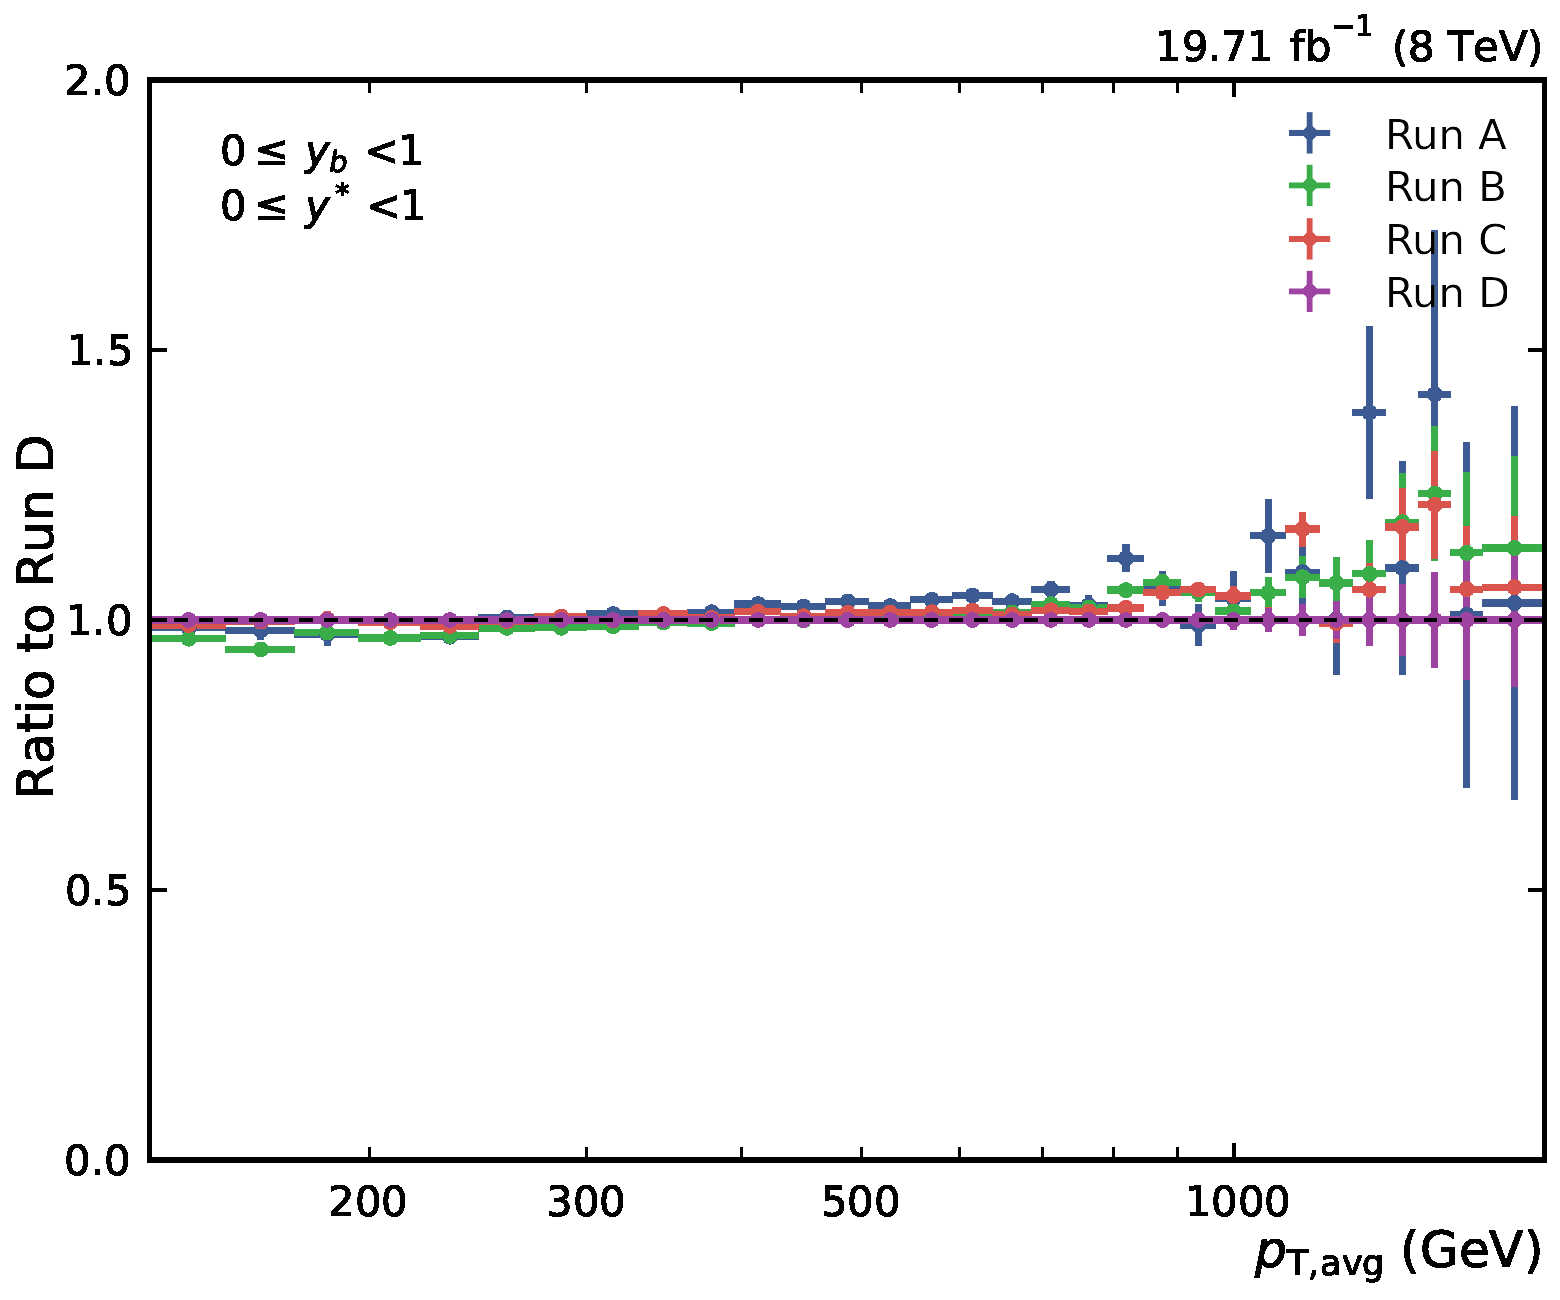
\includegraphics[width=0.47\textwidth]{figures/measurement/run_comparison_yb0ys0.pdf}\hfill
    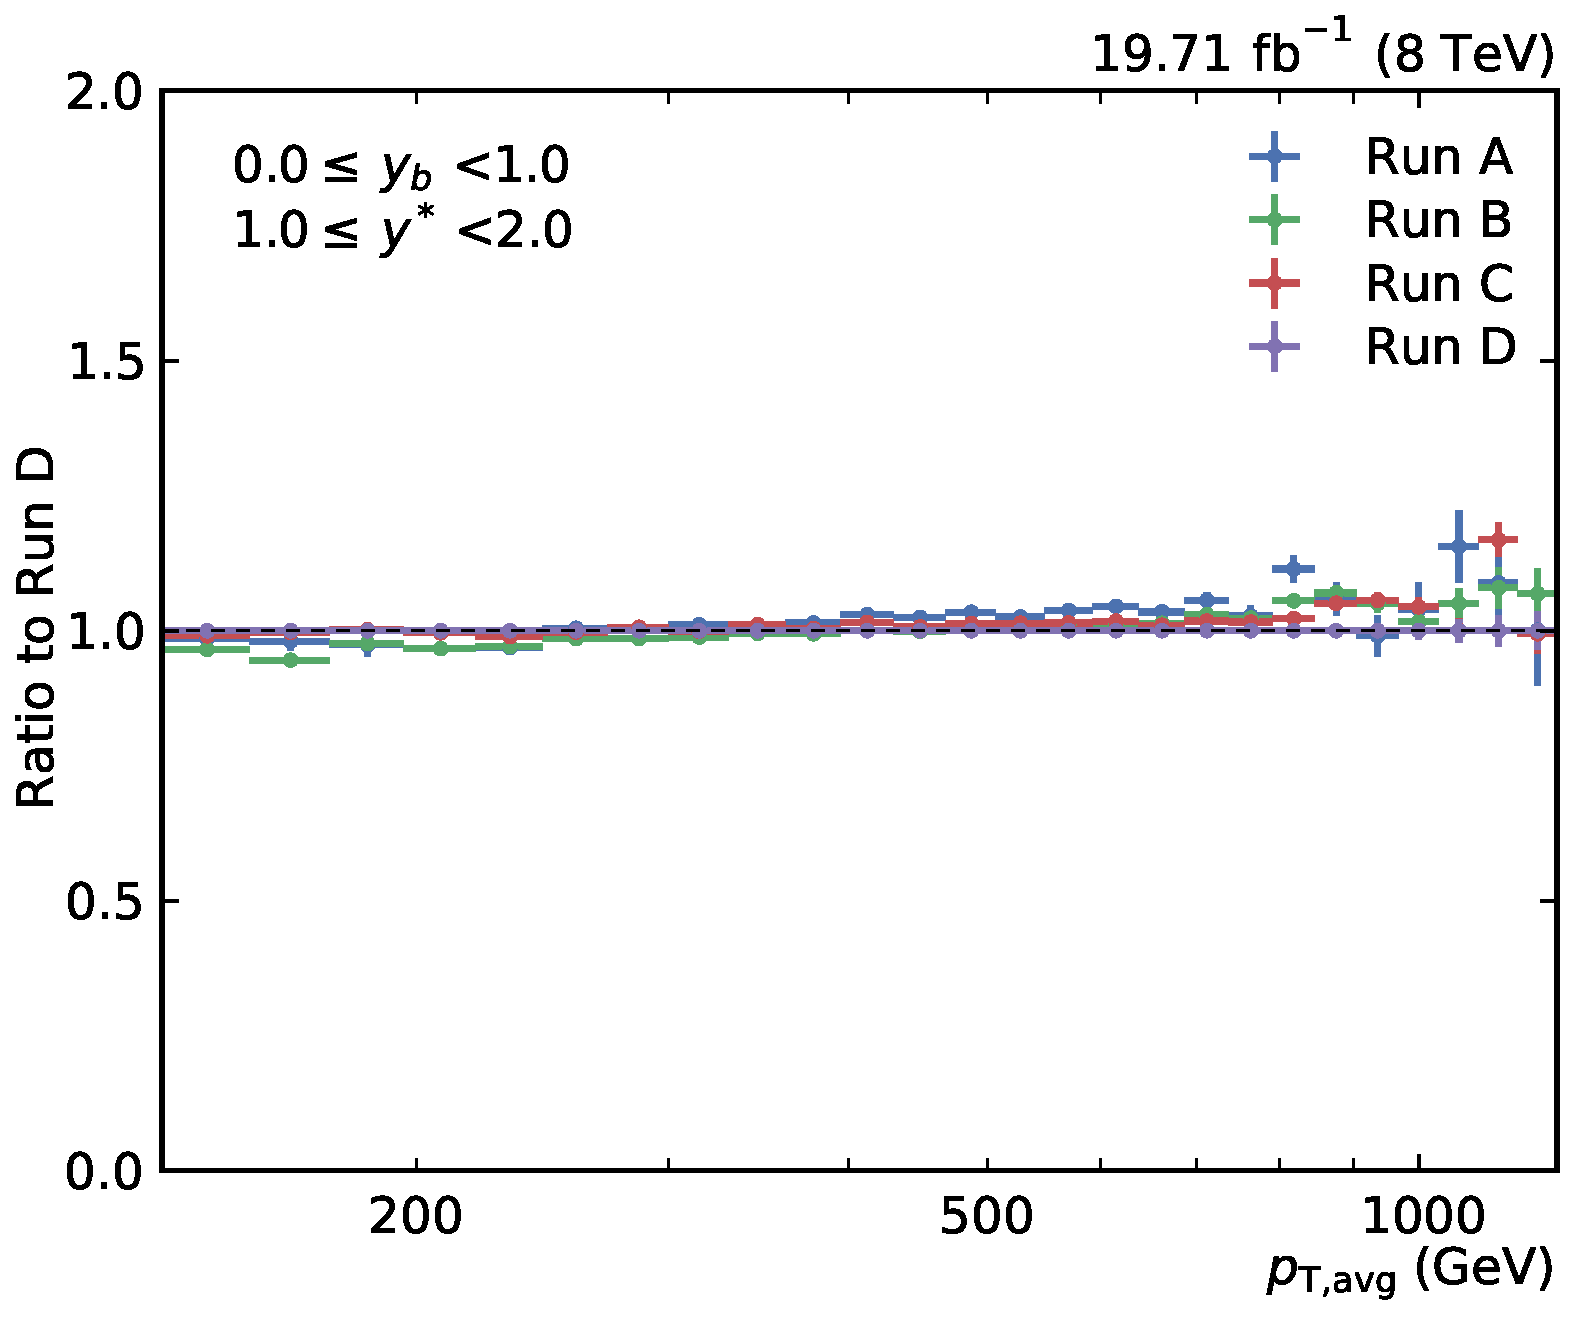
\includegraphics[width=0.47\textwidth]{figures/measurement/run_comparison_yb0ys1.pdf}
    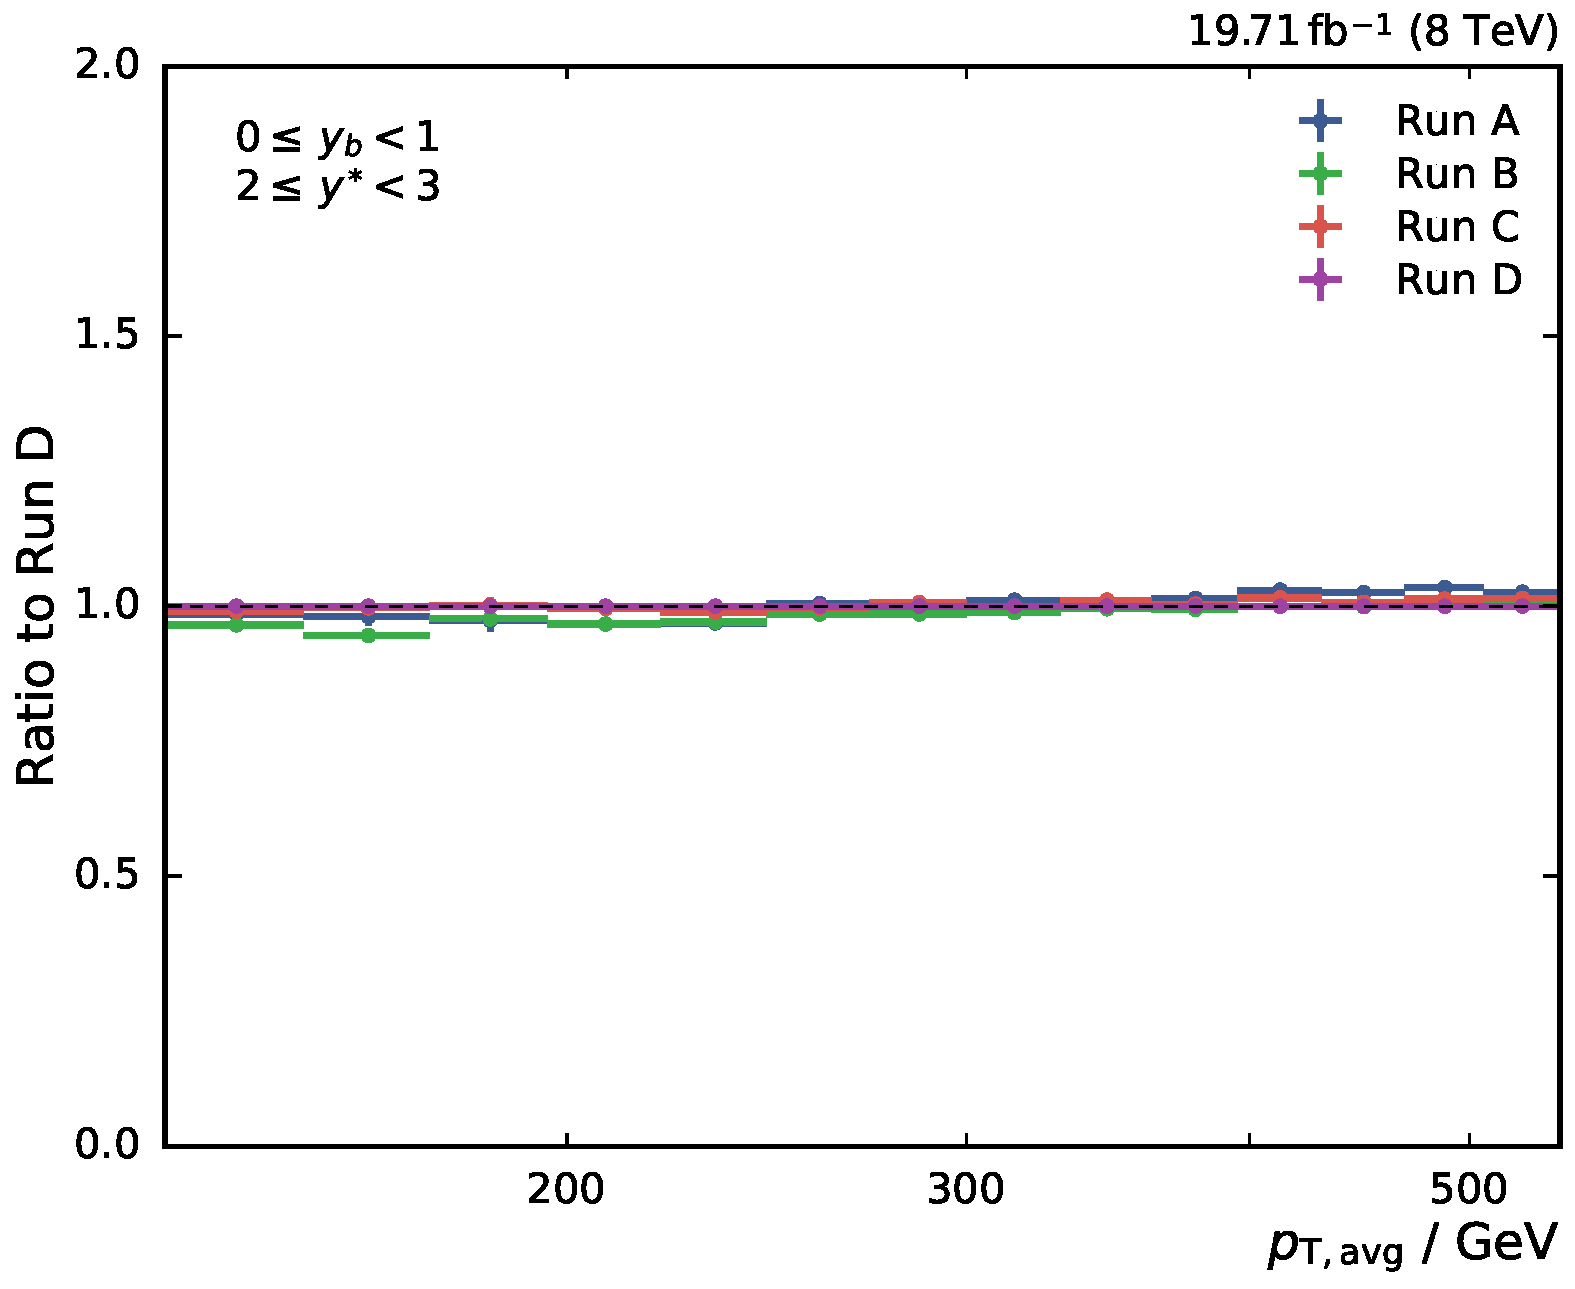
\includegraphics[width=0.47\textwidth]{figures/measurement/run_comparison_yb0ys2.pdf}\hfill
    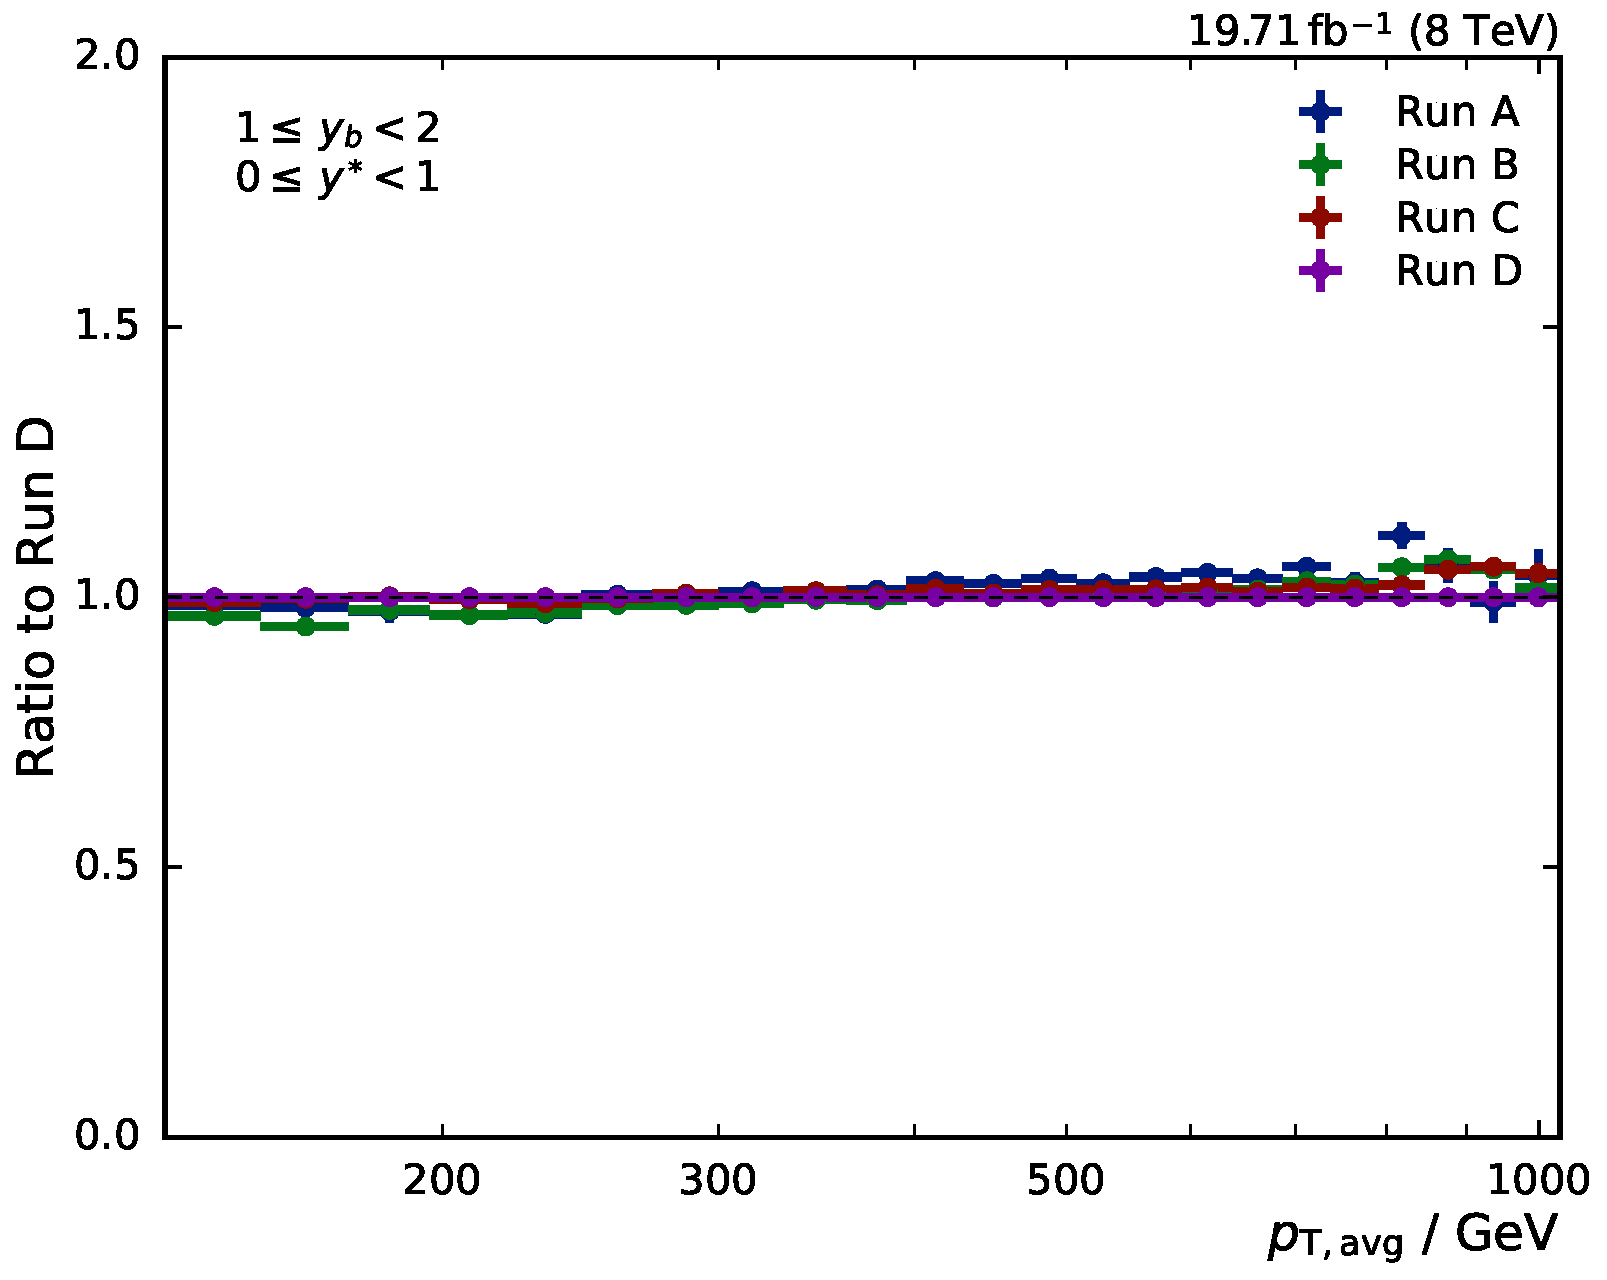
\includegraphics[width=0.47\textwidth]{figures/measurement/run_comparison_yb1ys0.pdf}
    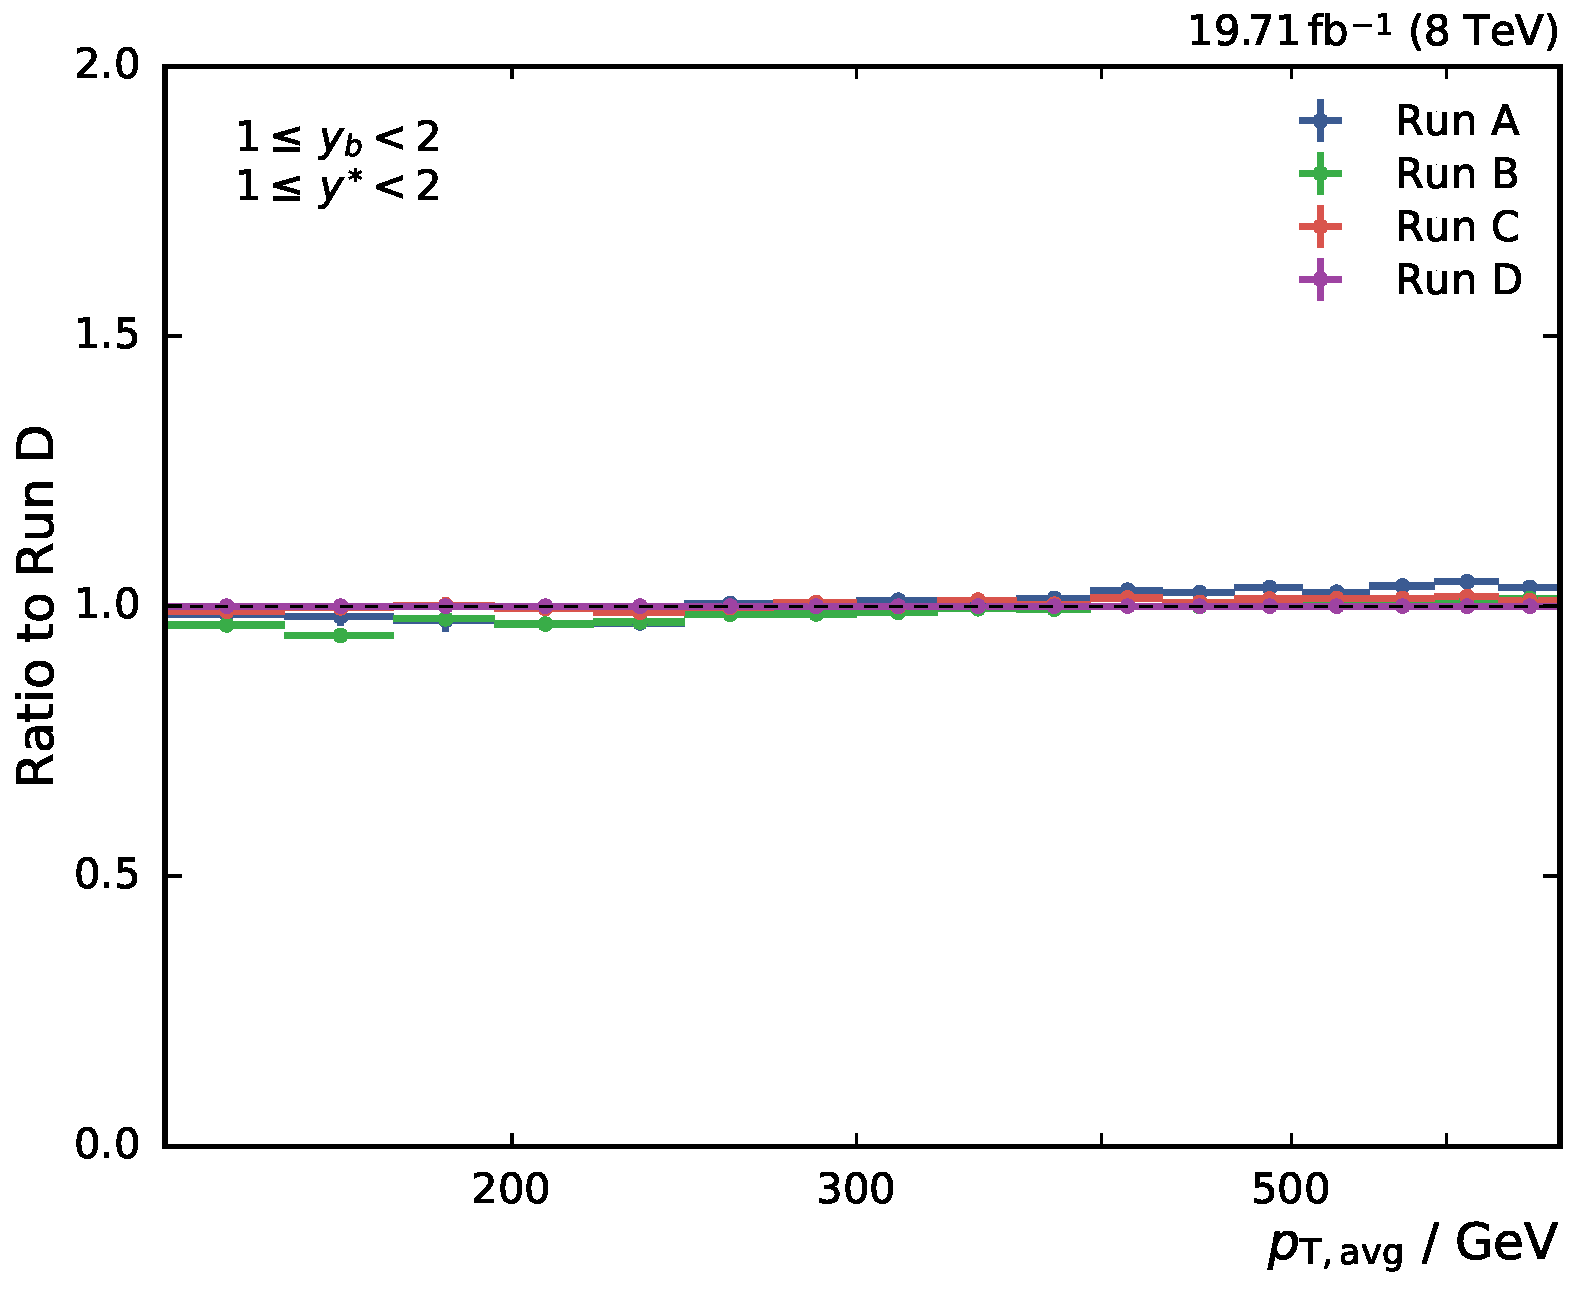
\includegraphics[width=0.47\textwidth]{figures/measurement/run_comparison_yb1ys1.pdf}\hfill
    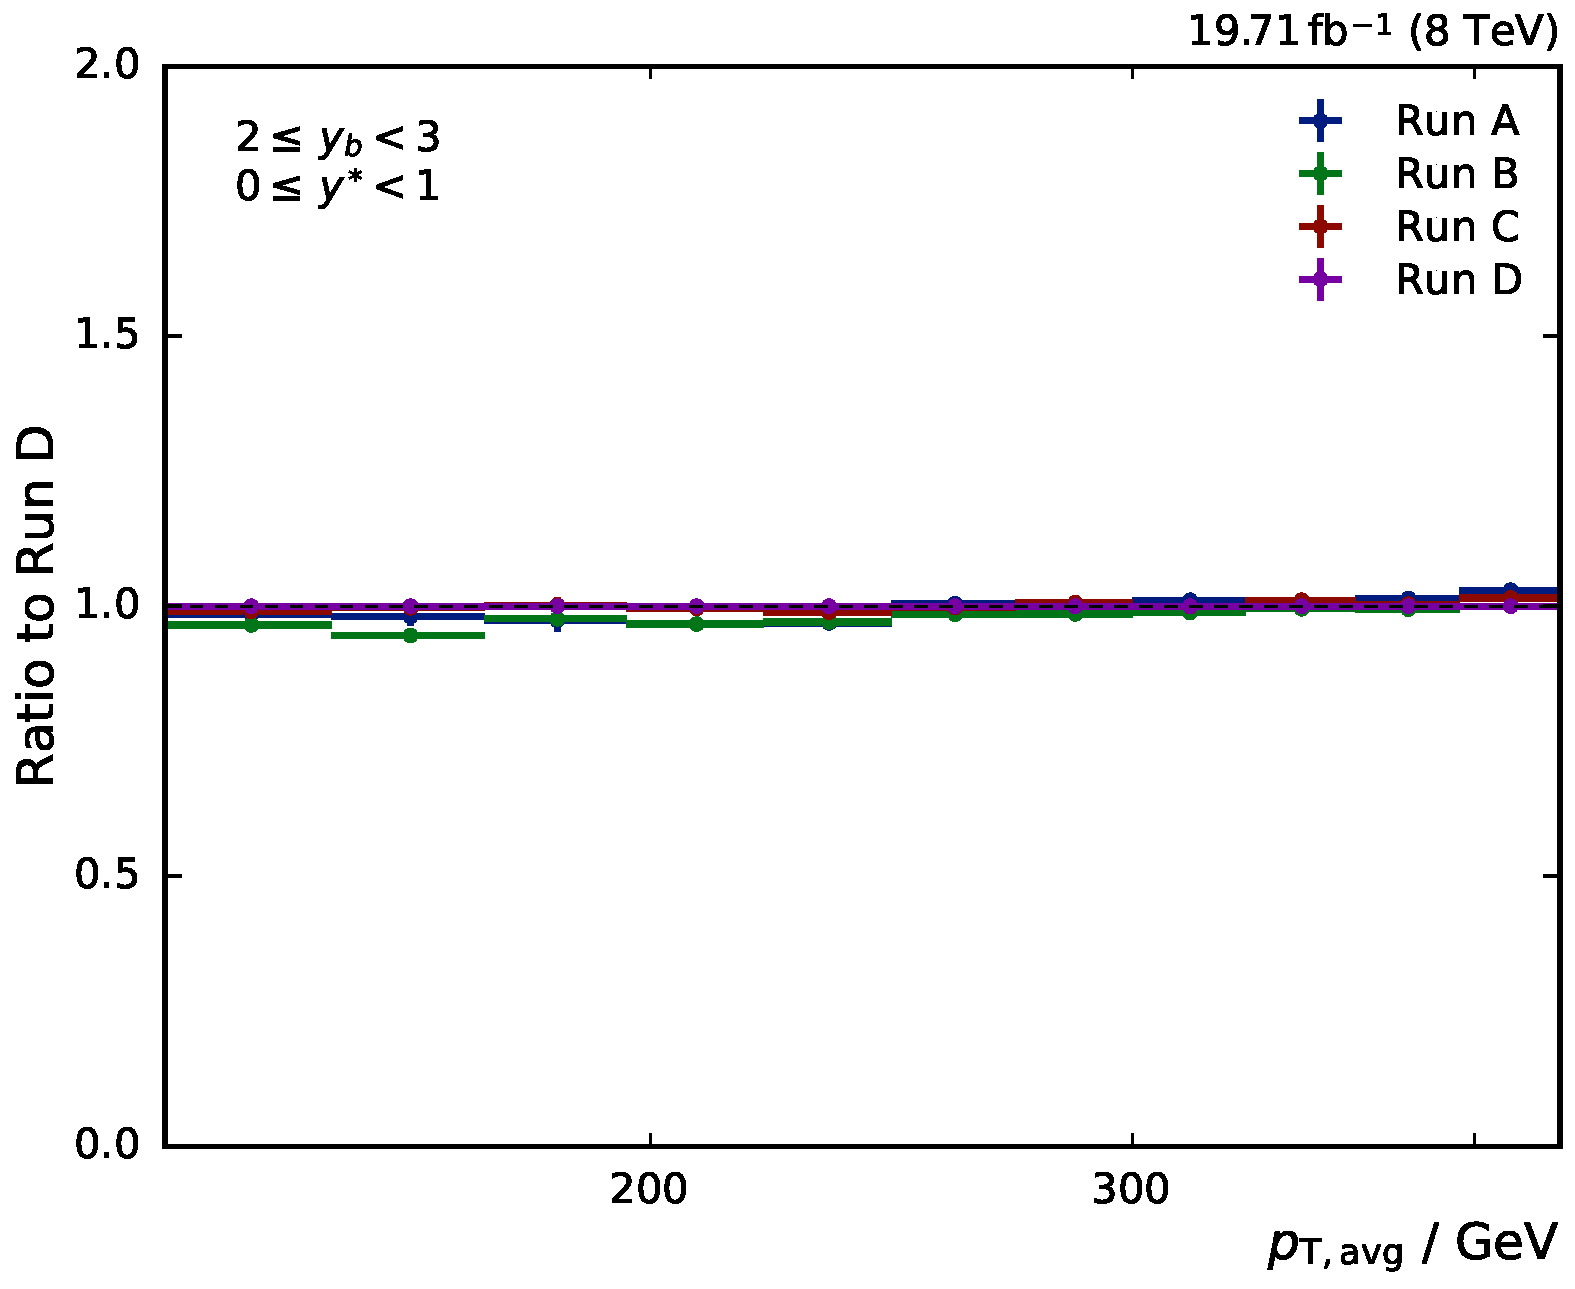
\includegraphics[width=0.47\textwidth]{figures/measurement/run_comparison_yb2ys0.pdf}
    \caption[Stability of result over all run periods]{Ratio of the measured
    cross section in each run period to the cross section obtained with data
    from Run D. There are small differences, mostly due to statistical fluctuations.
    A slight slope is observed for the result of run B, but overall separately
    obtained cross sections are in good agreement.}
    \label{fig:run_comparison}
\end{figure}

\section{Comparison with Simulated Events}
\label{sec:simulated_events}

\subsection{Pileup Reweighting}

The official Monte Carlo samples are enriched with an admixture of pileup
collisions to mimic the pileup distribution expected in data. Ideally, the
estimated pileup distribution in data $N_\mathrm{data} (N_\mathrm{PU, est.})$
would match with the simulated distribution $N_\mathrm{MC} (N_\mathrm{PU,
truth})$. Since the admixture is only a rough estimate of the pileup
distribution expected in the forthcoming data taking, a perfect matching cannot
be achieved. To still get comparable pileup distributions in data and simulated
events, the simulated events are reweighted with a weight $w_\mathrm{PU}$ to
match the distribution in data: 

\begin{equation*}
    w_{\mathrm{PU}} (N_{\mathrm{PU, truth}}) = \frac{N_\mathrm{data}
    (N_\mathrm{PU, est.}) / \sum N_\mathrm{data}}{N_\mathrm{MC}
    (N_\mathrm{PU, truth}) / \sum N_\mathrm{MC}}
\end{equation*}

Fig.~\ref{fig:mc:npv_reweighting} shows the number of reconstructed vertices
before and after reweighting. The significant mismatch of the
pileup distributions in data and simulated events, which can be observed before
reweighting the simulated events, vanishes.

\begin{figure}[htbp]
    \centering
    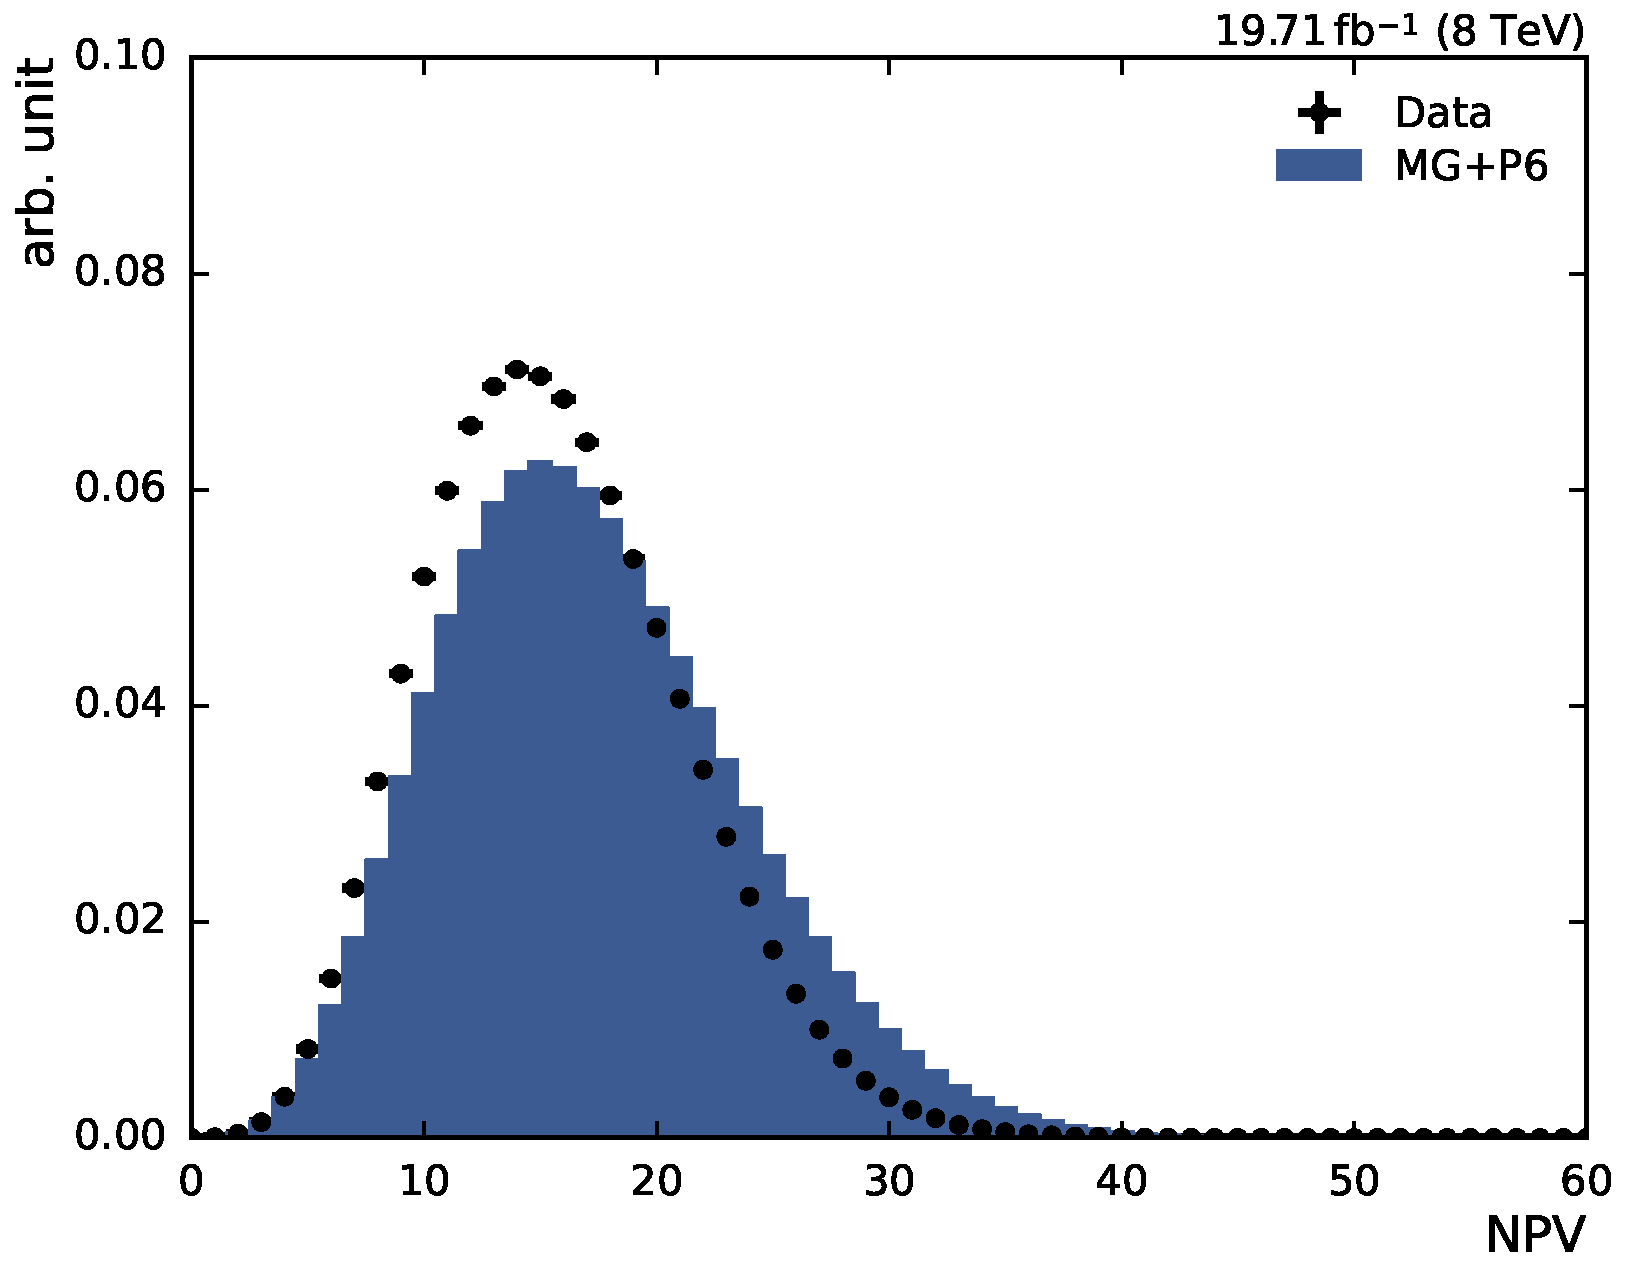
\includegraphics[width=0.47\textwidth]{figures/measurement/npv_beforereweighting.pdf}\hfill
    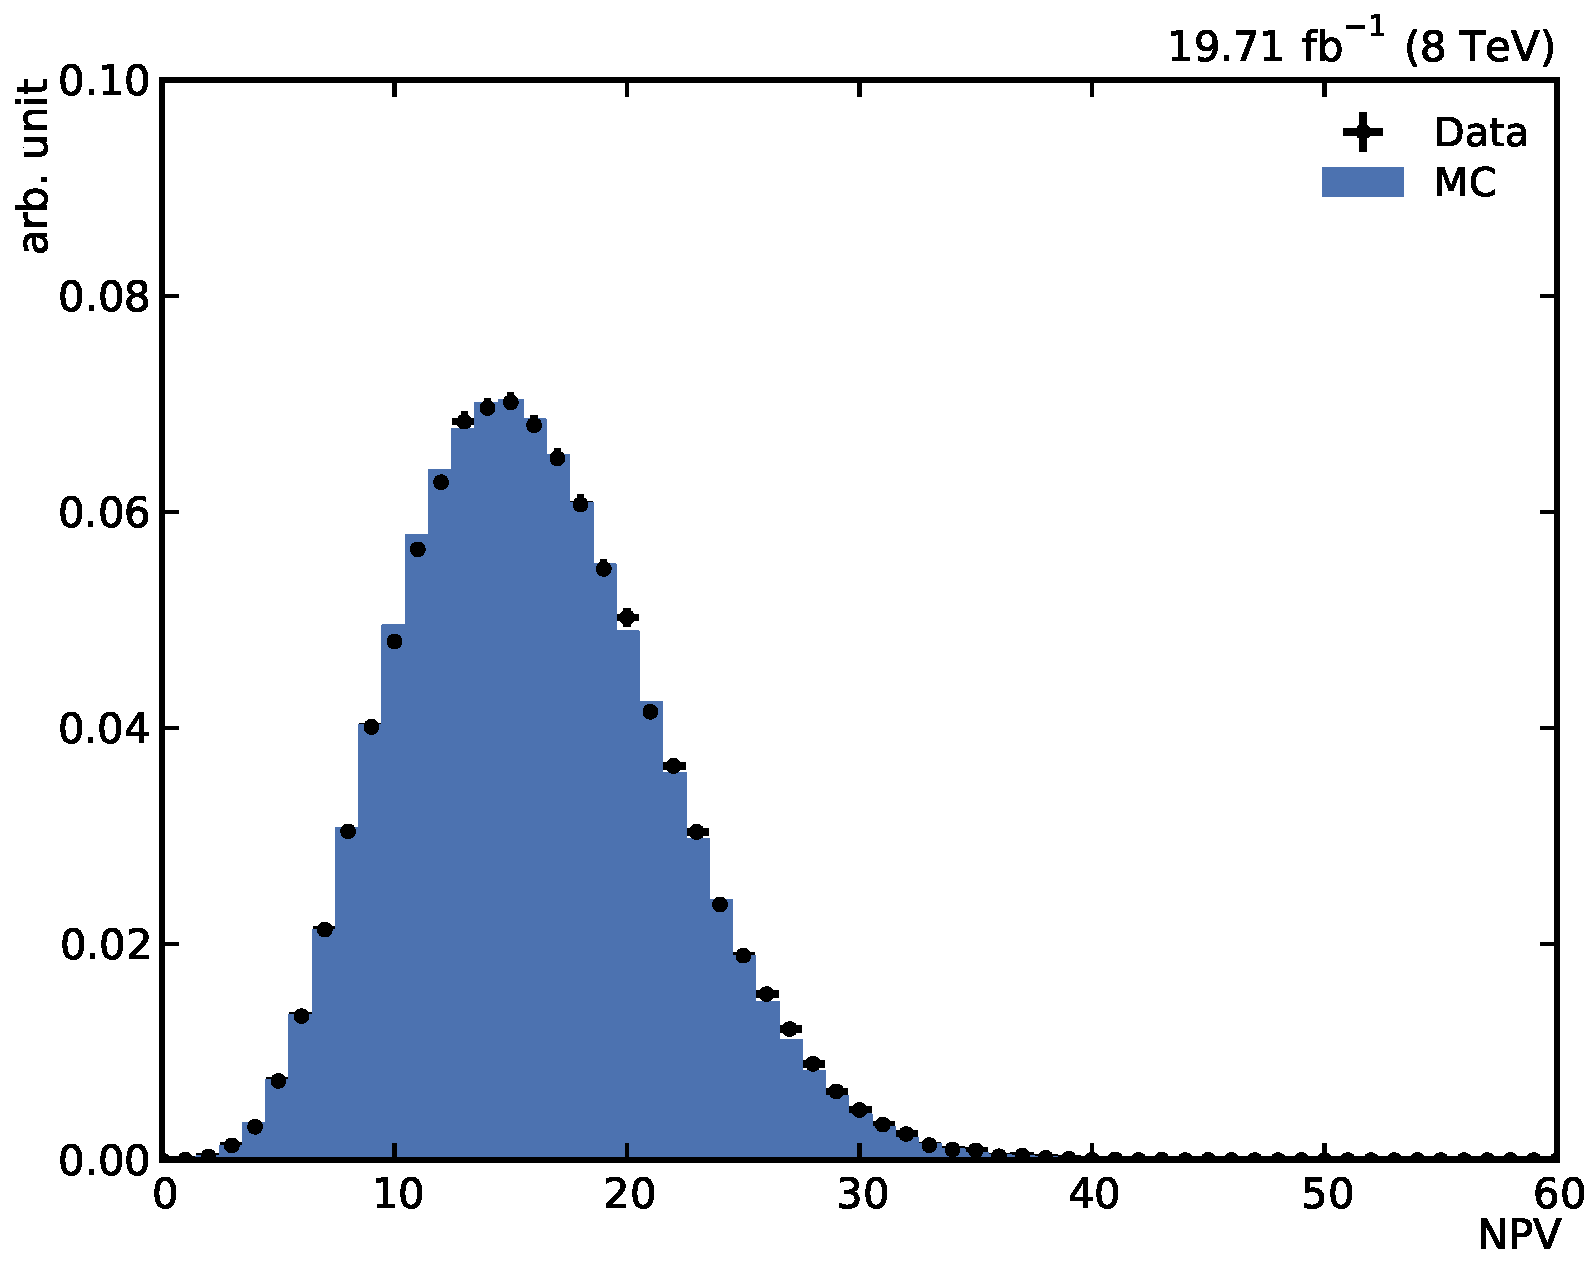
\includegraphics[width=0.47\textwidth]{figures/measurement/npv_afterreweighting.pdf}
    \caption[Number of reconstructed vertices]{Number of reconstruced vertices in data and simulated events before
    (left) and after (right) the pileup reweighting.}
    \label{fig:mc:npv_reweighting}
\end{figure}

\subsection{Kinematic distributions}

Kinematic quantities of dijet events are compared with simulated events on
reconstructed level. To achieve that, the generated events were processed
through the complete detector simulation and reconstruction.
Figure~\ref{fig:controlplots:kinematic} shows the transverse momentum $\pt$, the
rapidity $y$ and the azimuthal angle $\phi$ for the leading two jets. The
\pt-distribution is not that well described especially in the lower \pt region.
While the rapidity distribution is well described within the tracker coverage of
$y \approx 2.4$, there are larger discrepancices at higher rapidities.

\begin{figure}[htbp]
    \centering
    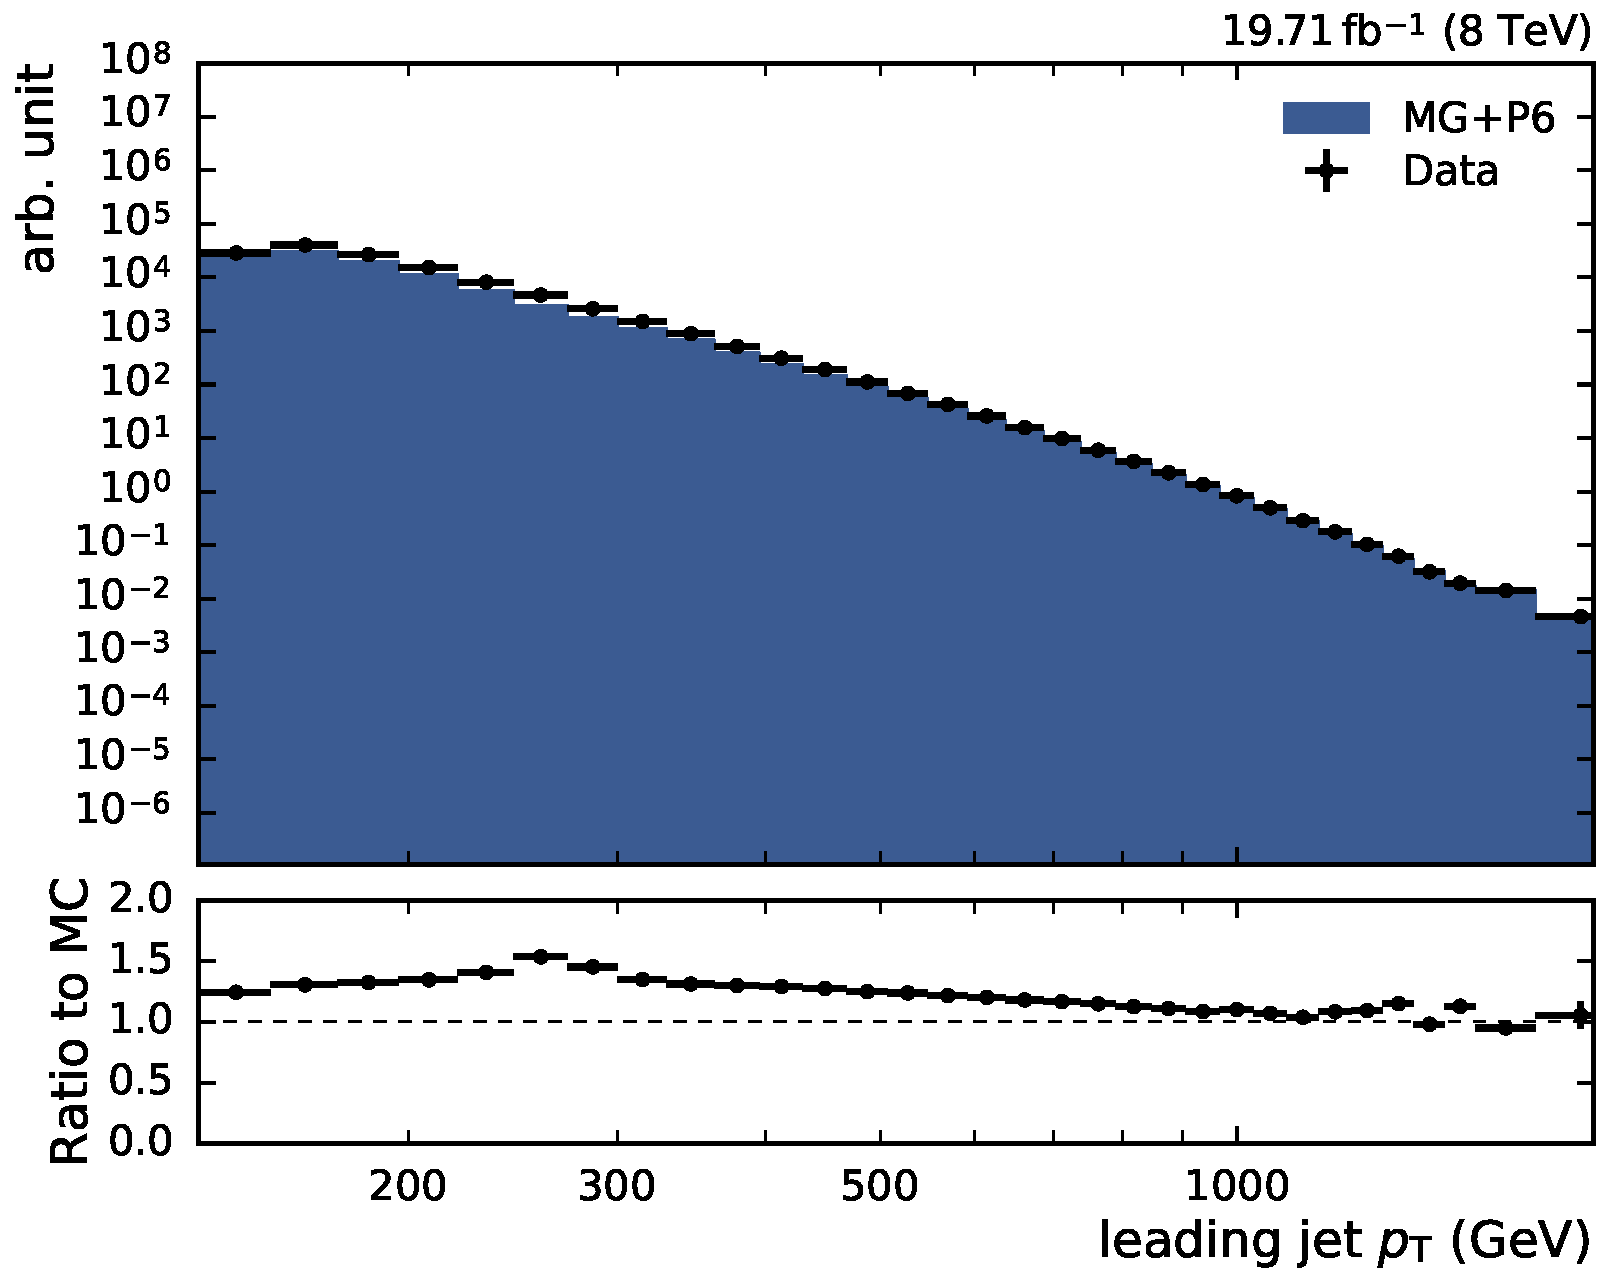
\includegraphics[width=0.47\textwidth]{figures/measurement/jet_quantities_jet1pt.pdf}\hfill
    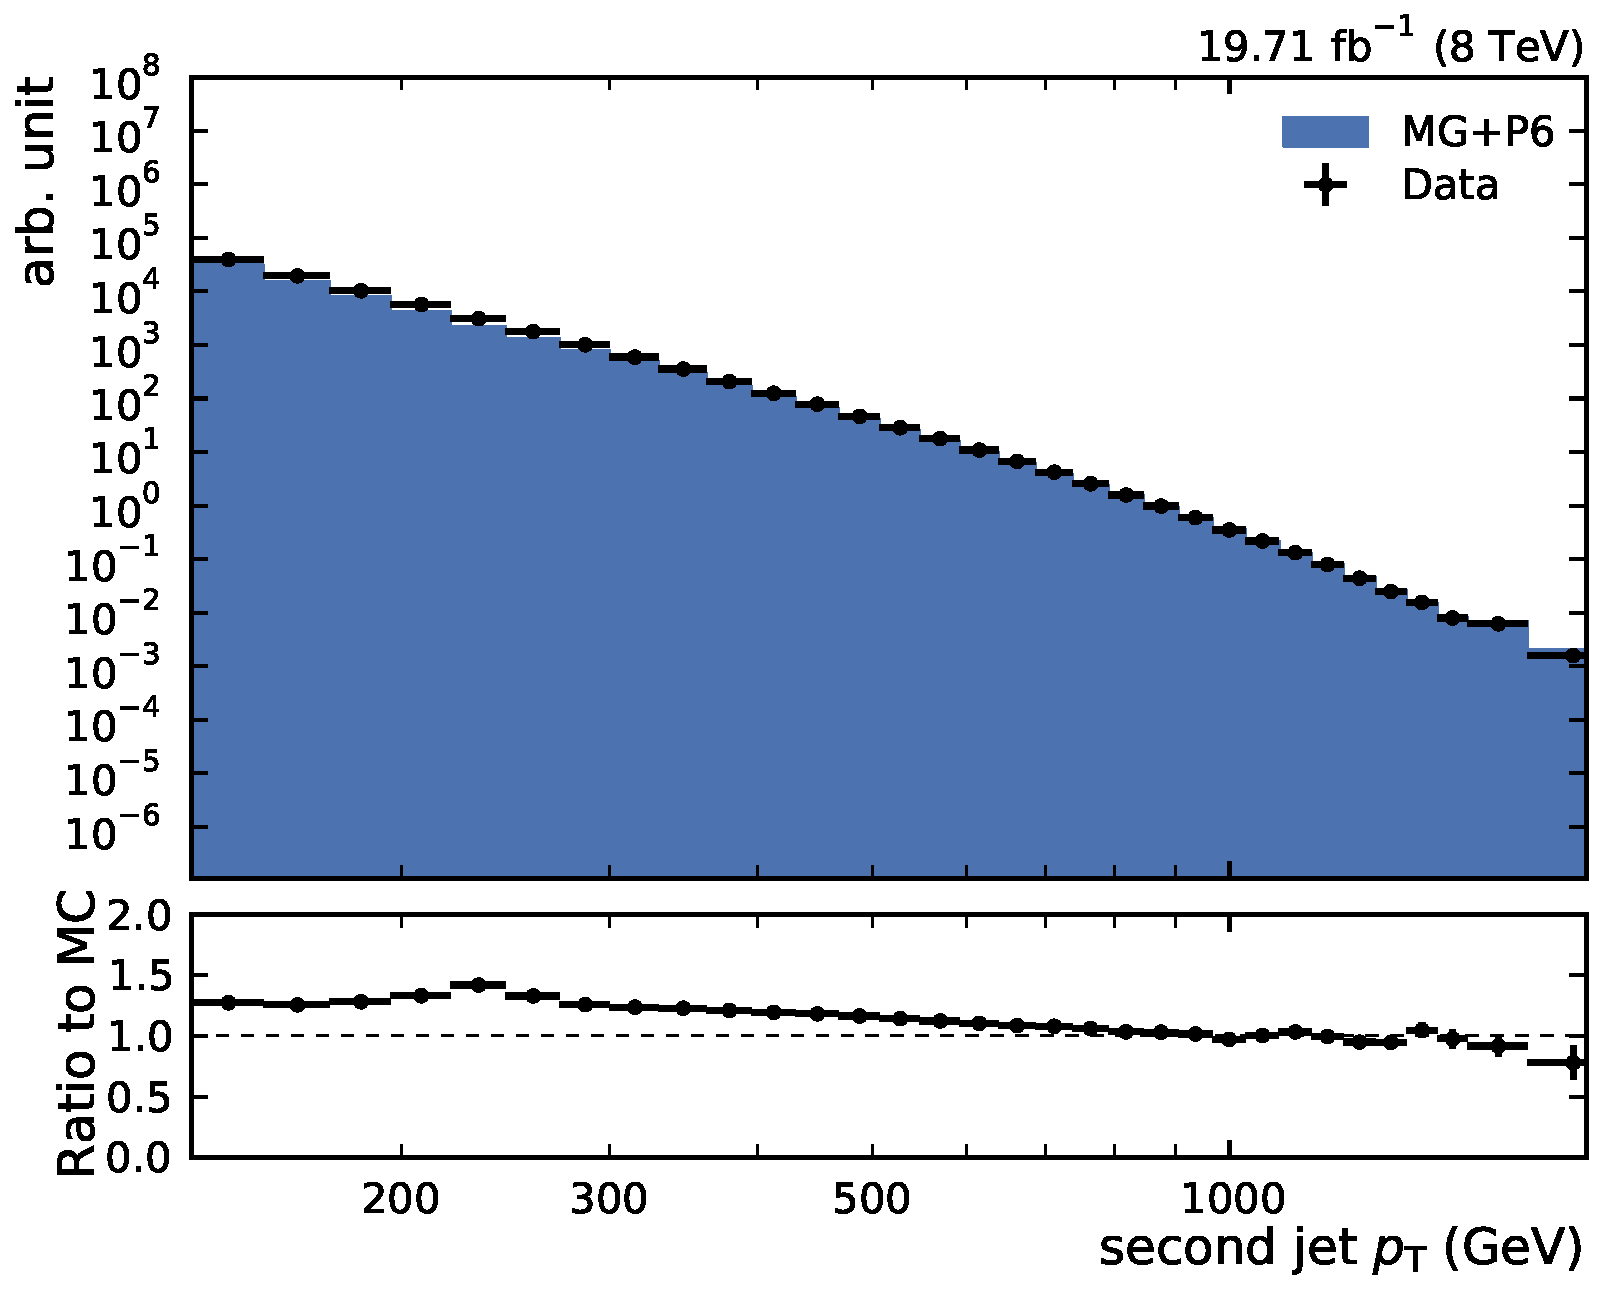
\includegraphics[width=0.47\textwidth]{figures/measurement/jet_quantities_jet2pt.pdf}
    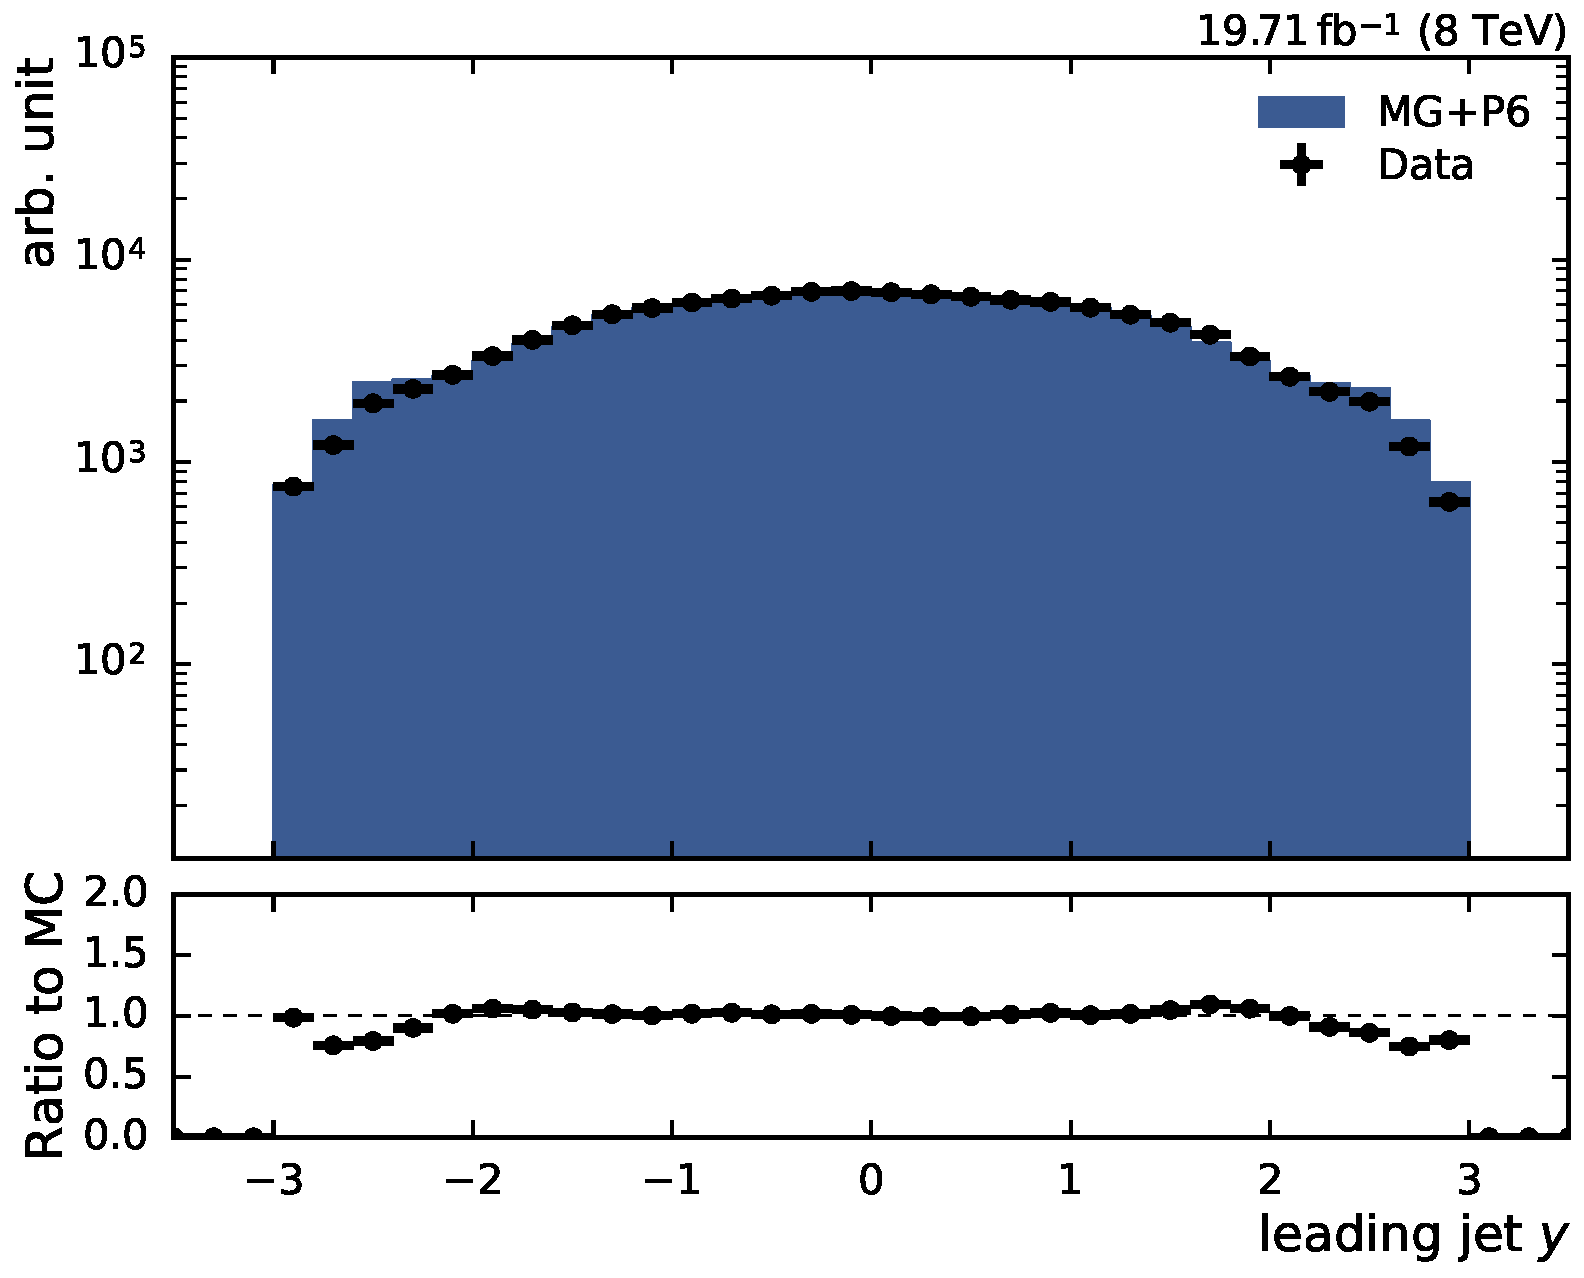
\includegraphics[width=0.47\textwidth]{figures/measurement/jet_quantities_jet1rap.pdf}\hfill
    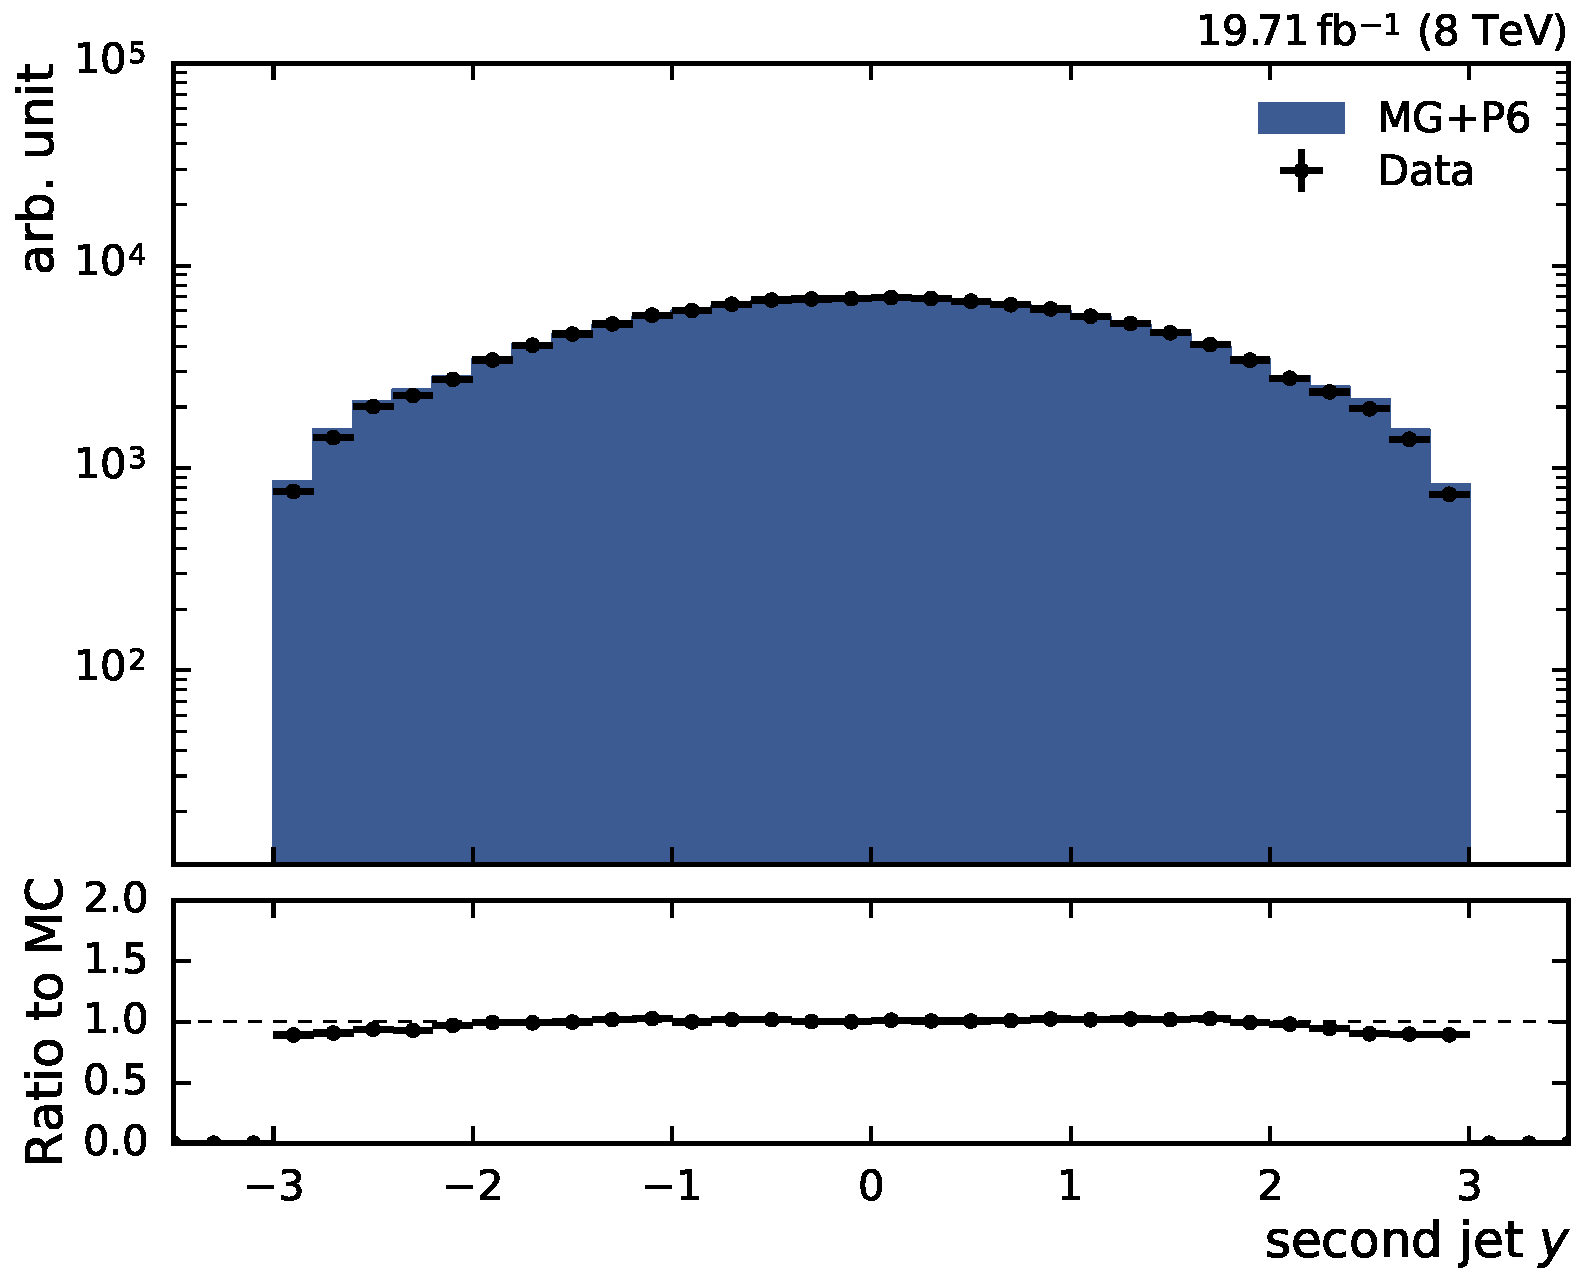
\includegraphics[width=0.47\textwidth]{figures/measurement/jet_quantities_jet2rap.pdf}
    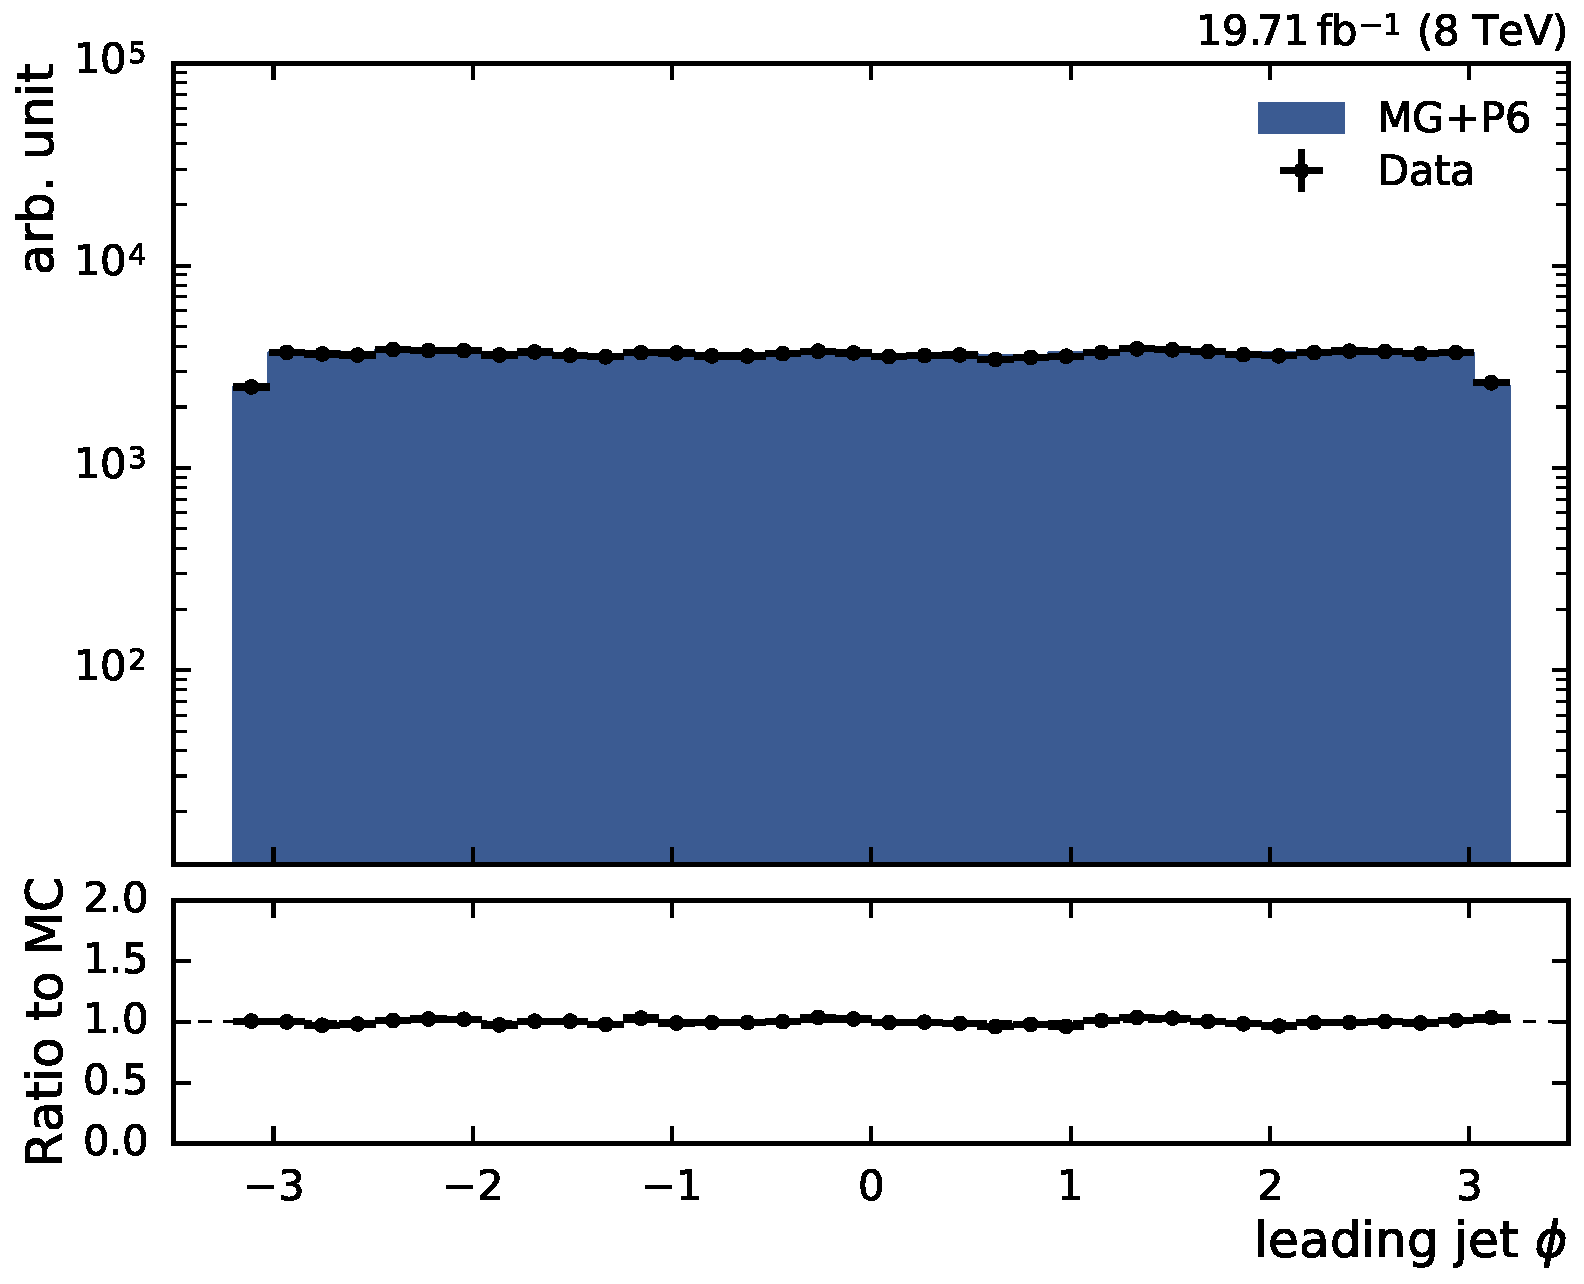
\includegraphics[width=0.47\textwidth]{figures/measurement/jet_quantities_jet1phi.pdf}\hfill
    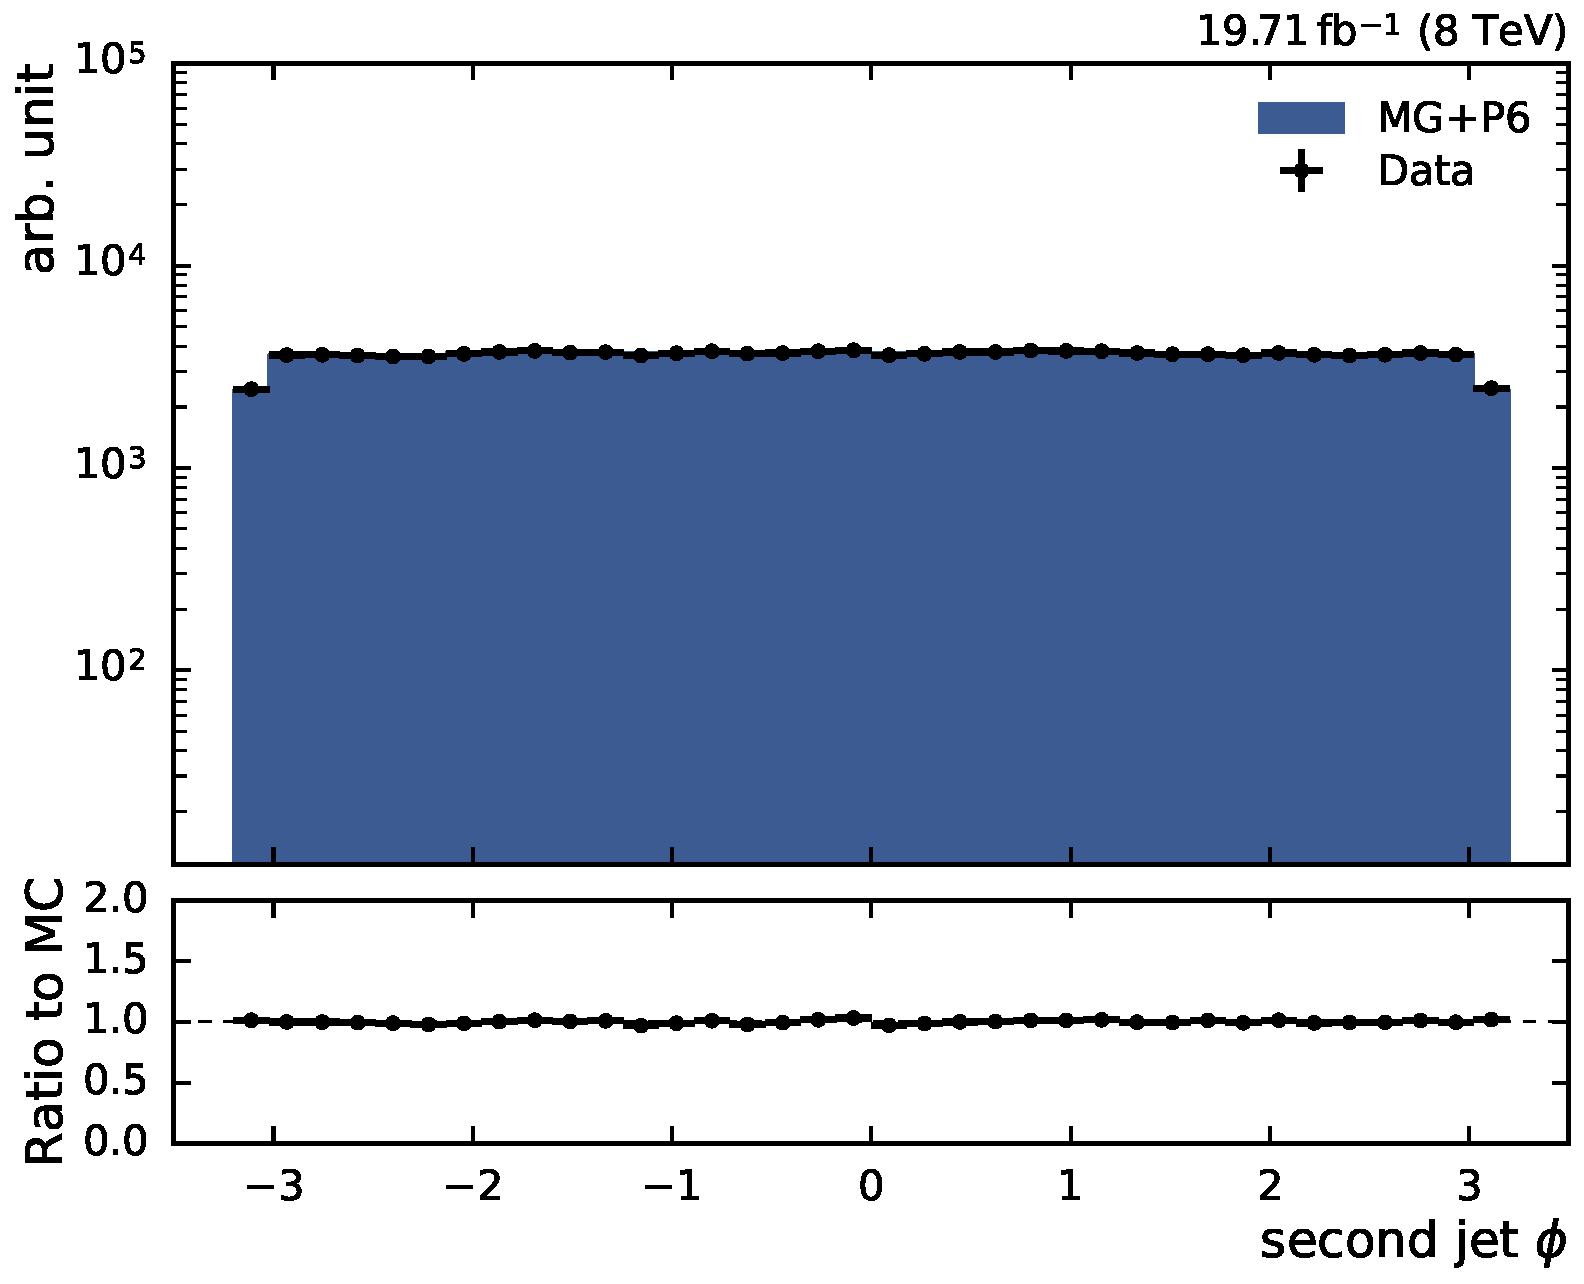
\includegraphics[width=0.47\textwidth]{figures/measurement/jet_quantities_jet2phi.pdf}
    \caption[Kinematic quantities of the jets]{The 
        kinematic quantities of the two leading jets are shown for the leading
        jet (left) and the second jet (right) both for data (markers) and
        simulated events (solid). The transverse momentum of the
        jets is shown in the top row, the rapdity in the middle row. The
        azimuthal angle of the jets is shown the bottom row.}
    \label{fig:controlplots:kinematic}
\end{figure}

\todo{text for dijet quantities}
\begin{figure}[htbp]
    \centering
    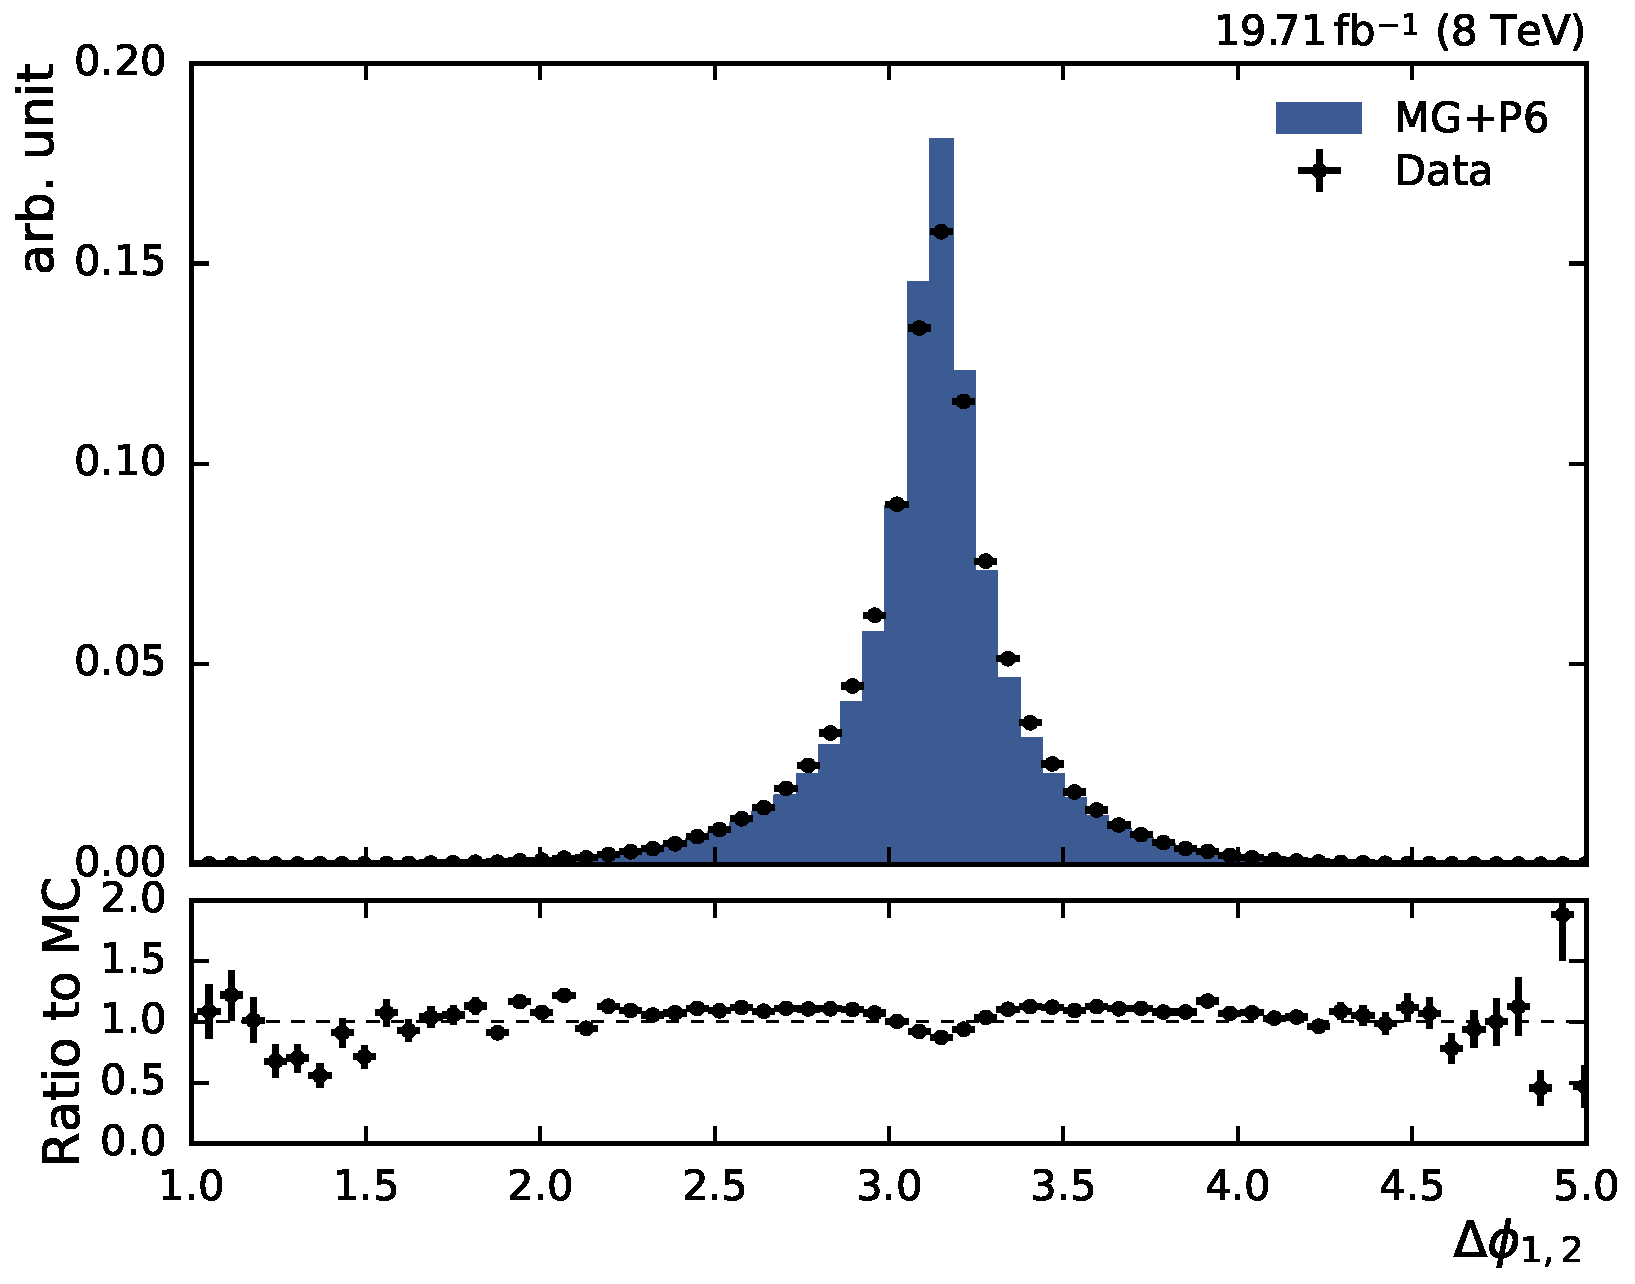
\includegraphics[width=0.47\textwidth]{figures/measurement/dijet_quantities_dijet_deltaphi.pdf}\hfill
    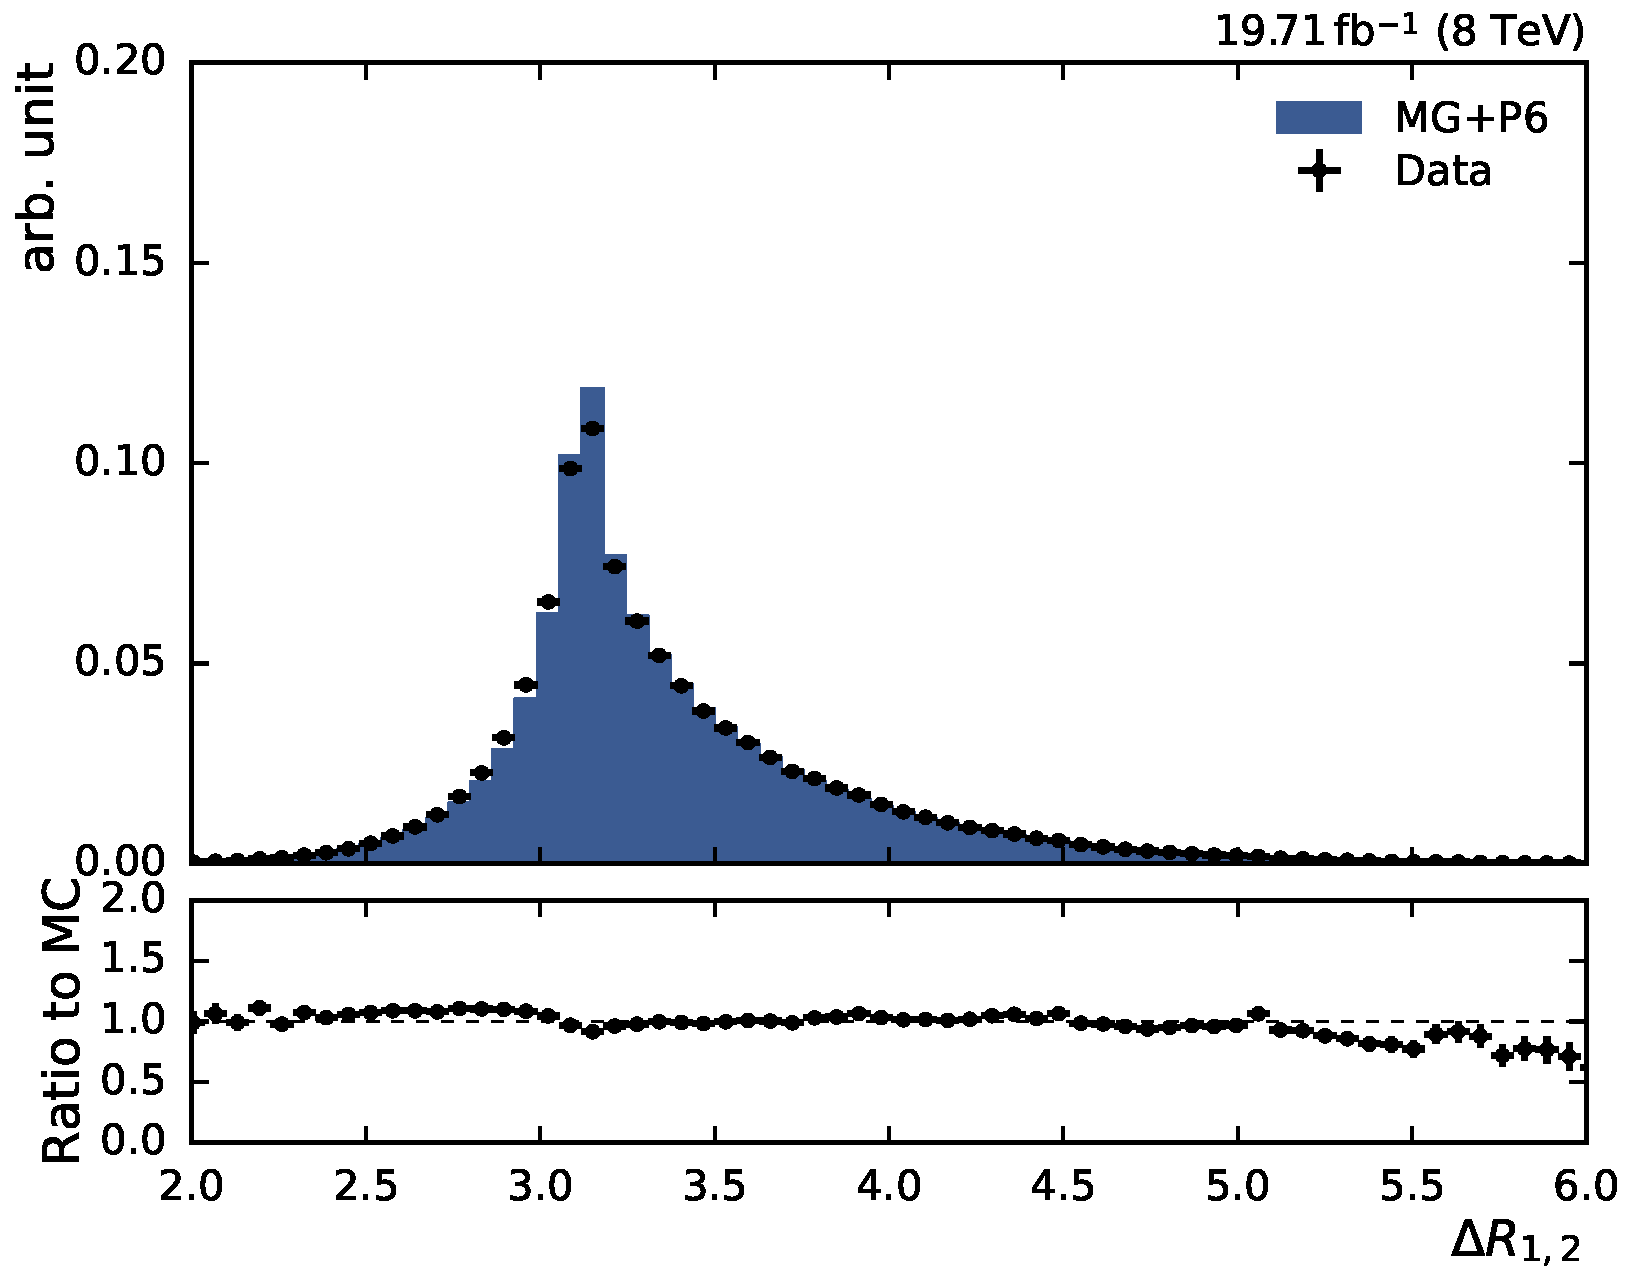
\includegraphics[width=0.47\textwidth]{figures/measurement/dijet_quantities_dijet_deltar.pdf}
    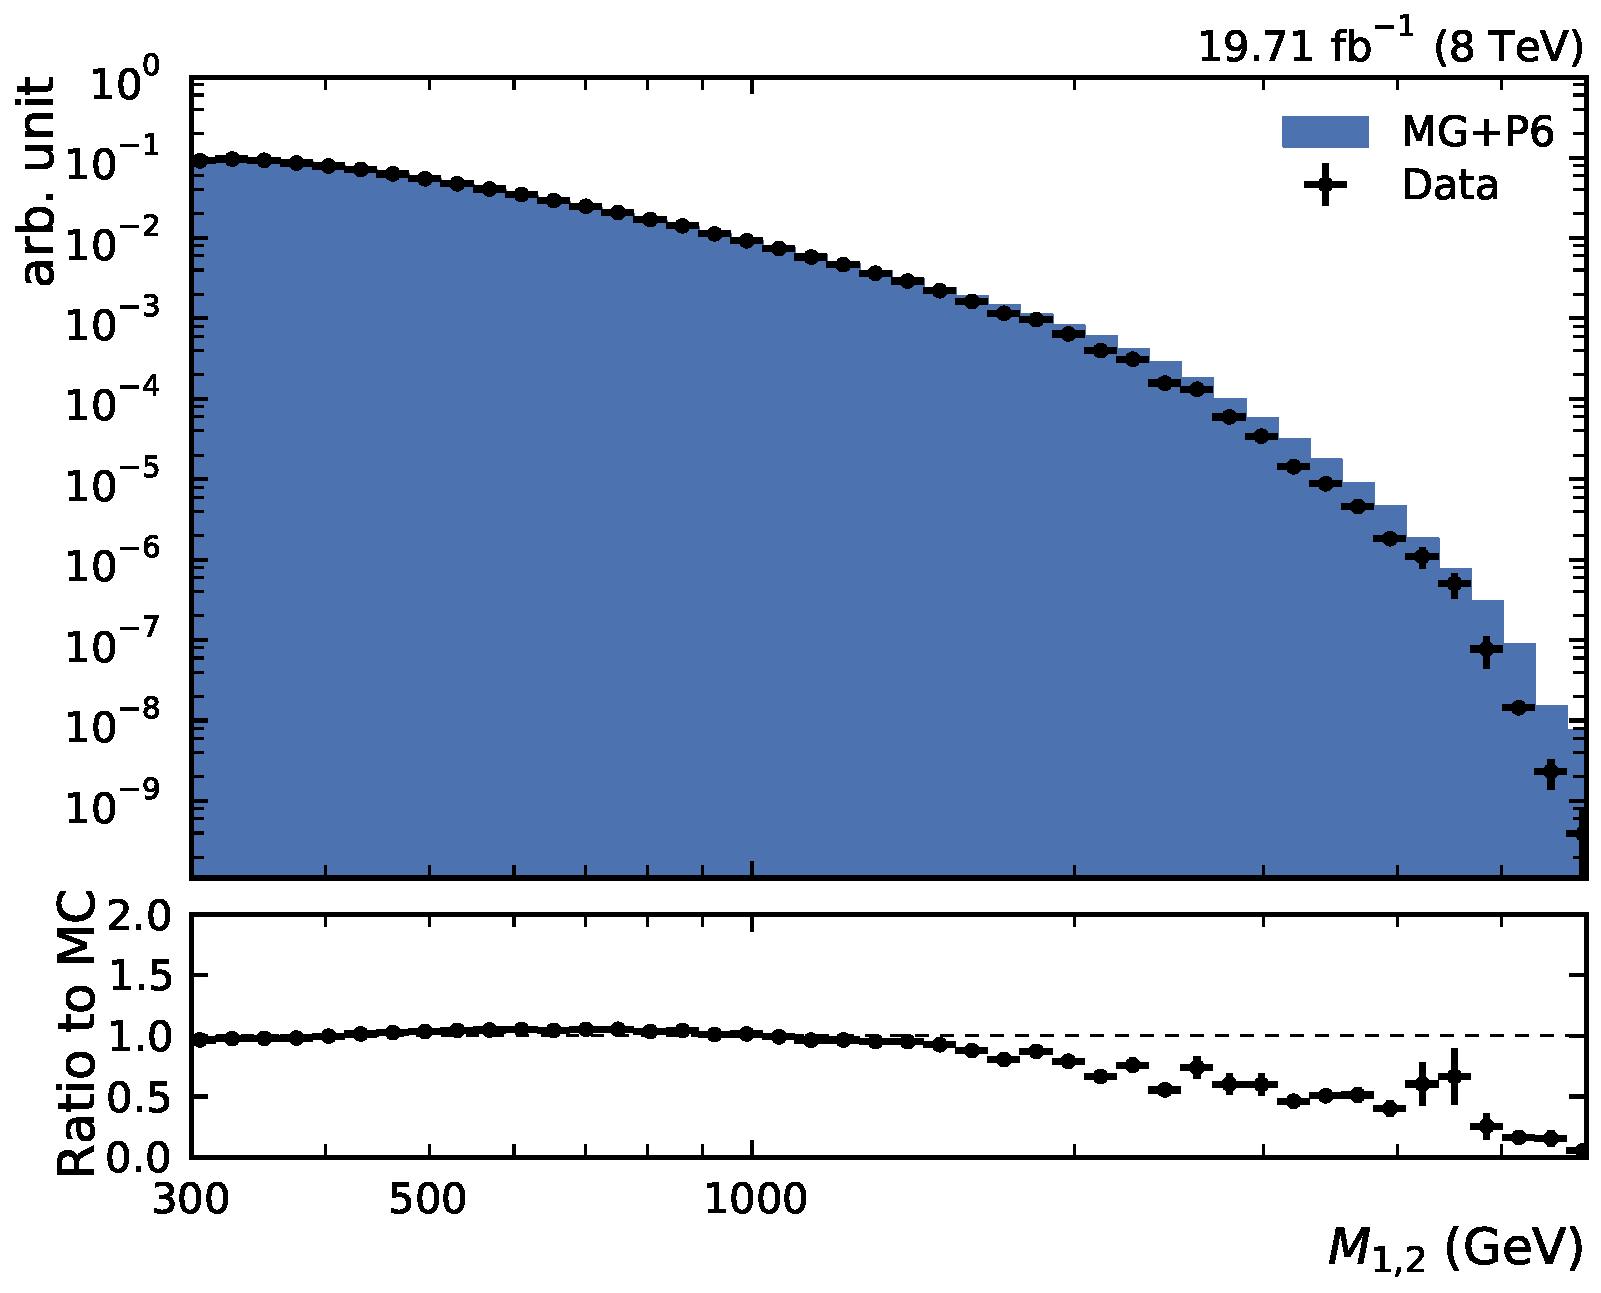
\includegraphics[width=0.47\textwidth]{figures/measurement/dijet_quantities_dijet_mass.pdf}\hfill
    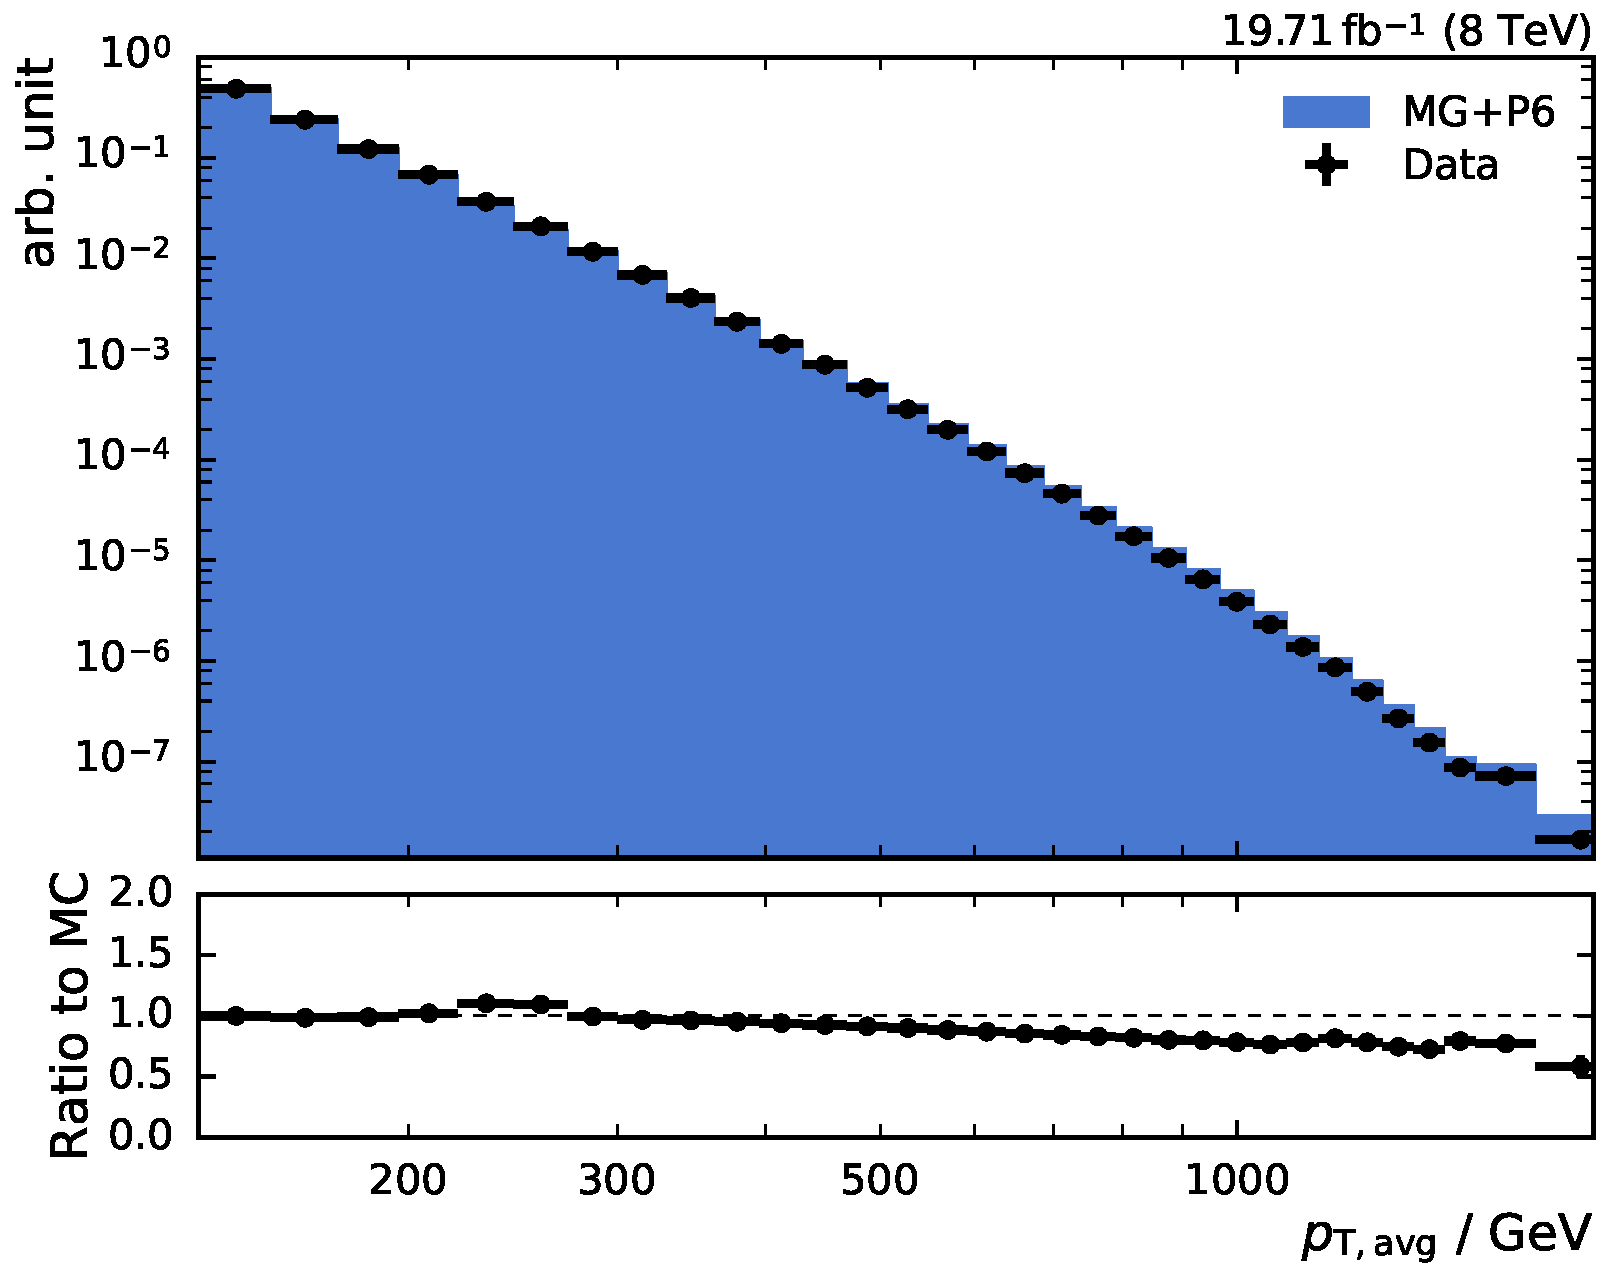
\includegraphics[width=0.47\textwidth]{figures/measurement/dijet_quantities_ptavg.pdf}
    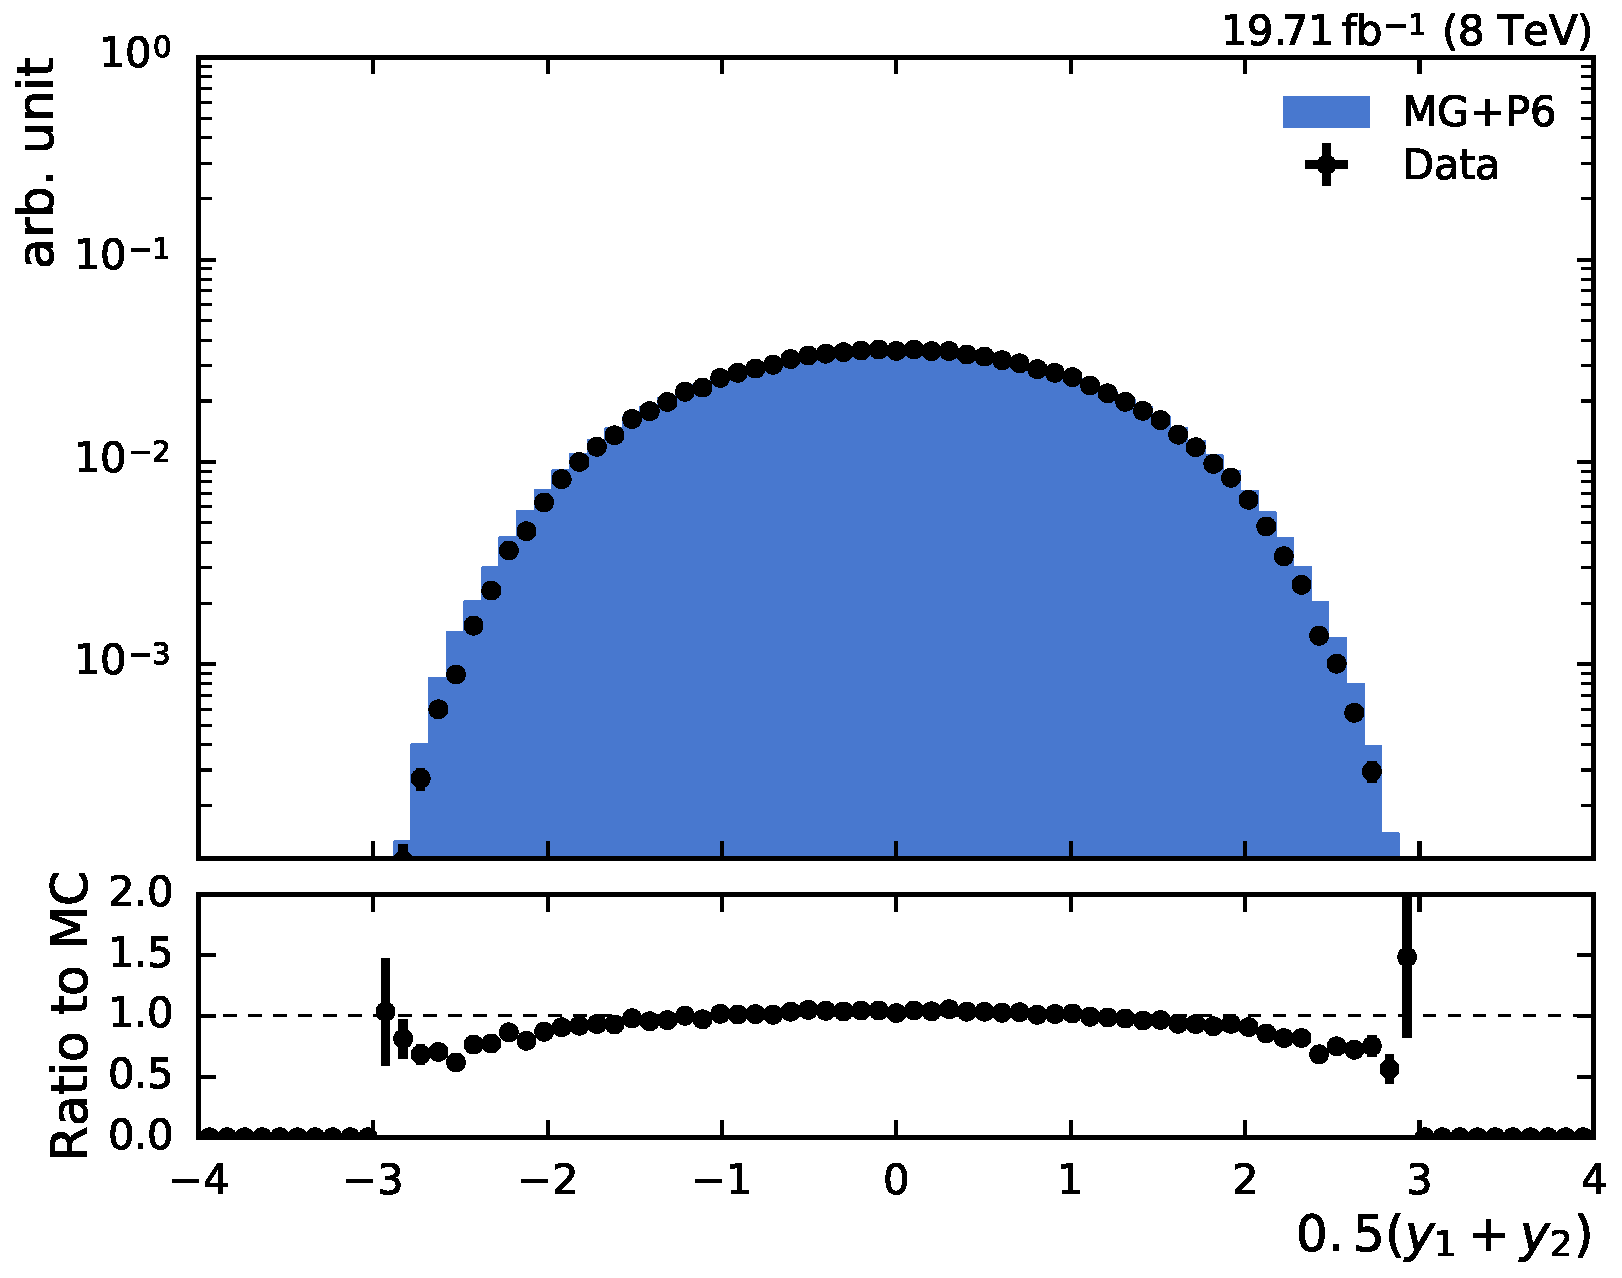
\includegraphics[width=0.47\textwidth]{figures/measurement/dijet_quantities_dijet_yboost.pdf}\hfill
    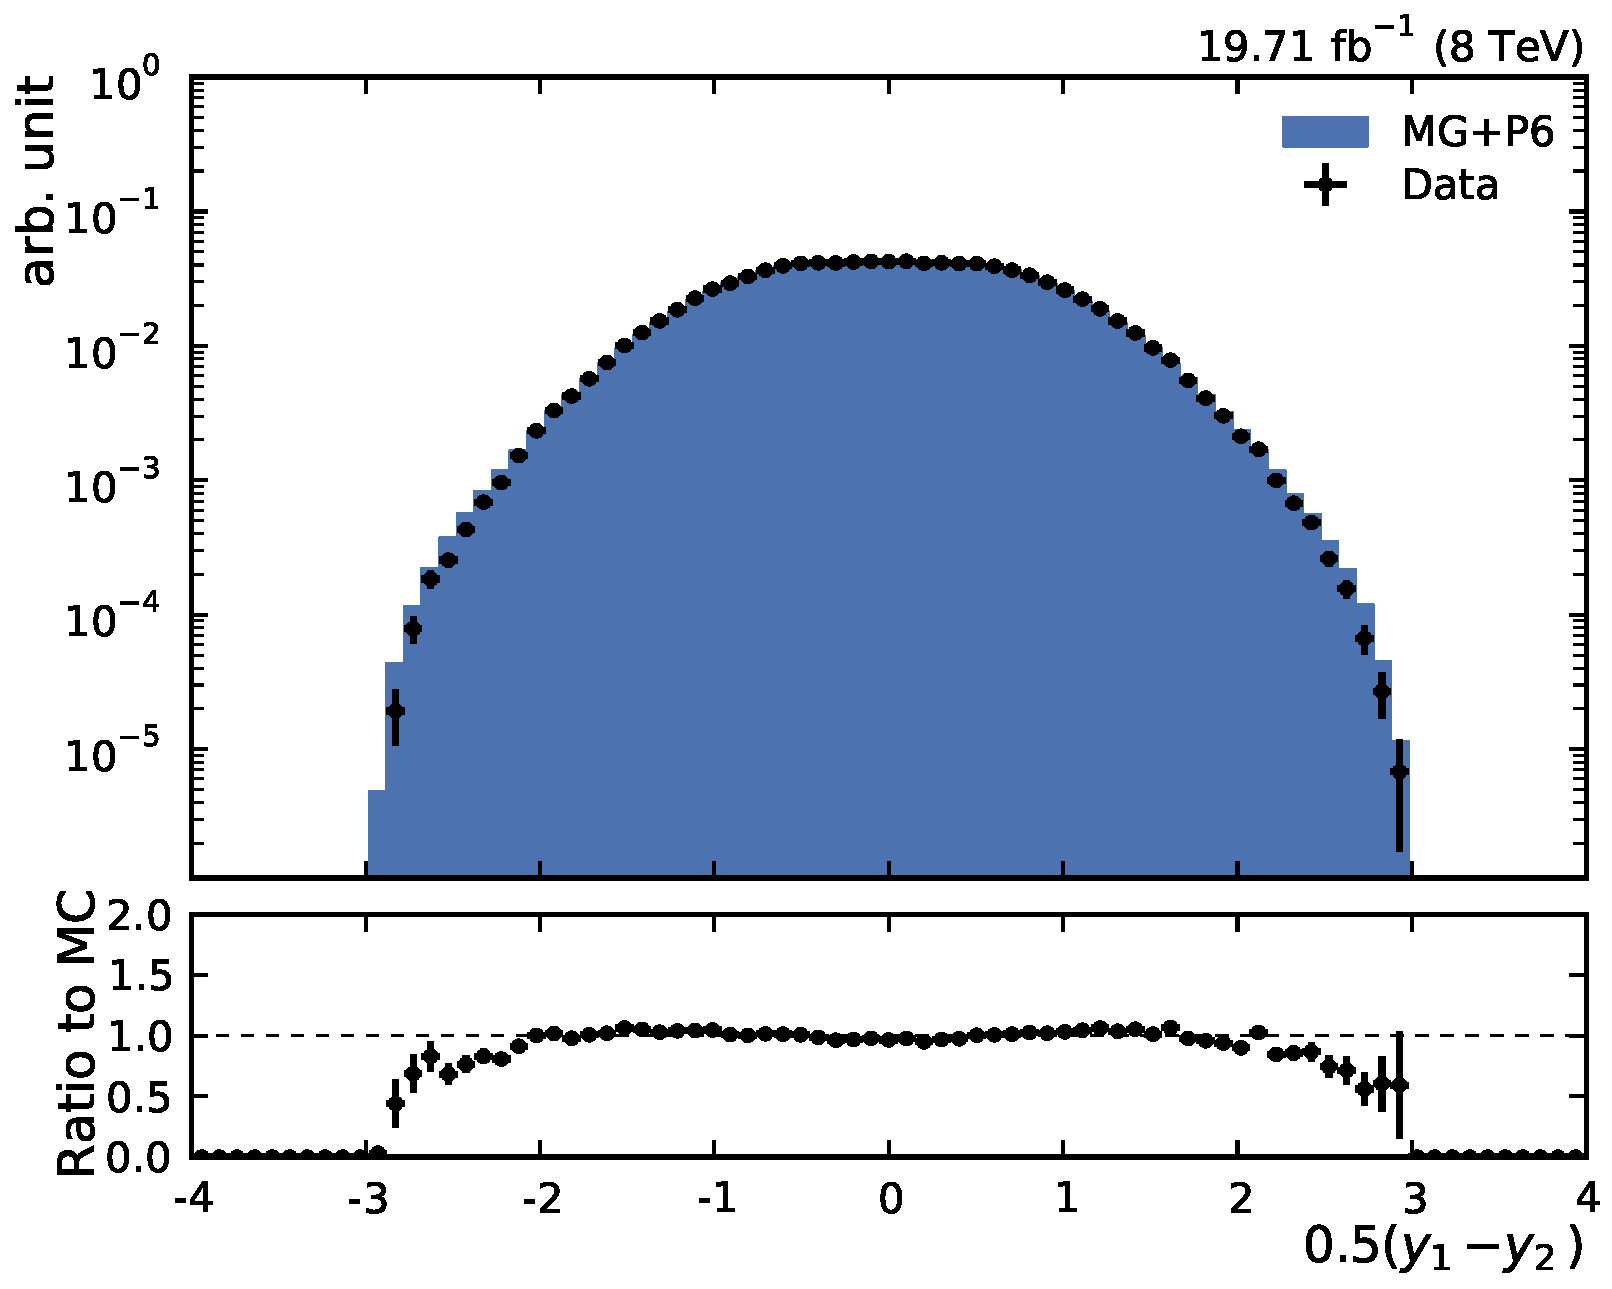
\includegraphics[width=0.47\textwidth]{figures/measurement/dijet_quantities_dijet_ystar.pdf}
    \caption[Kinematic quantities of the dijet system]{Kinematic quantities of
    the dijet system are shown for data (markers) and simulated events. The
azimuthal distance $\Delta\phi$ and the distance in the $\phi$-$\eta$ plane
$\Delta R$ are shown in the top row. The dijet mass $M_{1,2}$ and the average
transverse momentum of the dijet system $\ptavg$ is shown in the middle row. The
rapidity separation $0.5(y_1 - y_2)$ and the boost $0.5(y_1+y_2)$ is shown in
the bottom row.}
    \label{fig:controlplots:dijets}
\end{figure}


To illustrate the origin of the dijets in the different \ystar and \yboost bin
of the measured, the two-dimensional distributions in
Fig.~\ref{fig:controlplots:rapidity} give the events as a function of the
leading and second jet in data.

\begin{figure}[htbp]
    \centering
    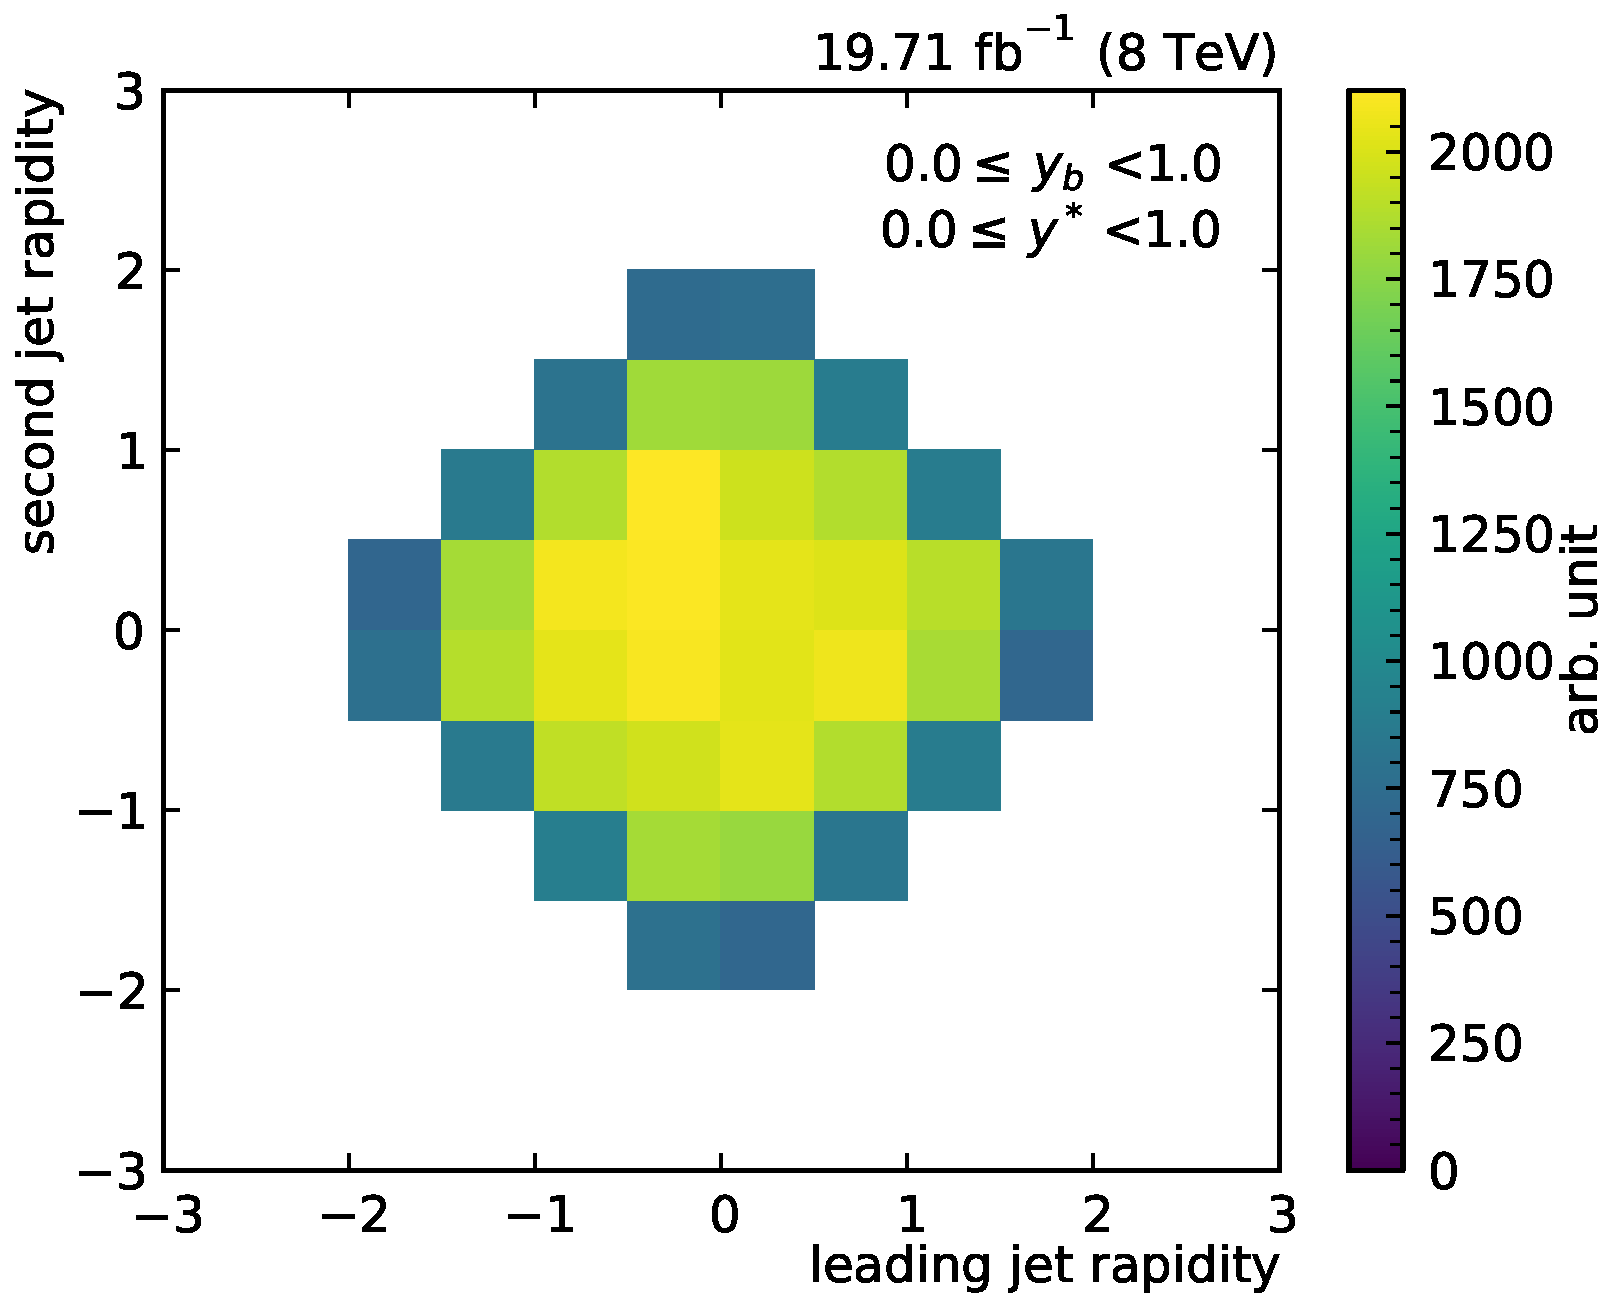
\includegraphics[width=0.47\textwidth]{figures/measurement/jet12_rapidity_yb0ys0.pdf}\hfill
    \includegraphics[width=0.47\textwidth]{figures/measurement/jet12_rapidity_yb0ys1.pdf}
    \includegraphics[width=0.47\textwidth]{figures/measurement/jet12_rapidity_yb0ys2.pdf}\hfill
    \includegraphics[width=0.47\textwidth]{figures/measurement/jet12_rapidity_yb1ys0.pdf}
    \includegraphics[width=0.47\textwidth]{figures/measurement/jet12_rapidity_yb1ys1.pdf}\hfill
    \includegraphics[width=0.47\textwidth]{figures/measurement/jet12_rapidity_yb2ys0.pdf}
    \caption[Rapidities of the two leading jets in the various \ystar and \yboost bins]{
             The distribution of the dijet events in the various \ystar and
             \yboost bins is shown as a function of the rapdities of the two jets.
             The color indicates the frequency distribution. The figures demonstrate the
             division of SS and OS dijet events, see \eg mid left and bottom right plot.}
    \label{fig:controlplots:rapidity}
\end{figure}

\subsection{Cross Section Comparison}

The Monte Carlo simulation is used to compare the prediction including the
detector simulation to the measured data distribution which is smeared due to
the finite detector resolution. Figure~\ref{fig:ratio_recotodata} shows the
prediction of the Madgraph and the Pythia 8 simulations as a ratio to the
measured data spectrum.  While the agreement in the inner detector region is
fine, the shape and especially the normalization of the MC prediction cannot
describe the data. Additionally, a fixed-order prediction of NLOJET++ is shown.
This prediction is on parton level and is not corrected for non-perturbative
effects. Still it describes best the data apart from the known effects due to NP
and detector resolution effects.

\begin{figure}[htbp]
    \centering
    \includegraphics[width=0.47\textwidth]{figures/measurement/ratio_reco_to_data_yb0ys0.pdf}\hfill
    \includegraphics[width=0.47\textwidth]{figures/measurement/ratio_reco_to_data_yb0ys1.pdf}
    \includegraphics[width=0.47\textwidth]{figures/measurement/ratio_reco_to_data_yb0ys2.pdf}\hfill
    \includegraphics[width=0.47\textwidth]{figures/measurement/ratio_reco_to_data_yb1ys0.pdf}
    \includegraphics[width=0.47\textwidth]{figures/measurement/ratio_reco_to_data_yb1ys1.pdf}\hfill
    \includegraphics[width=0.47\textwidth]{figures/measurement/ratio_reco_to_data_yb2ys0.pdf}
    \caption[Comparison of data with simulated events]{Comparison of the measurement and the predictions using P8 and MG+P6. The data distributions are normalized
    to the integrated luminosity, the simulated events to the number of generated events and the cross section. The ratio of the simulated
    events to the data points is shown.}
    \label{fig:ratio_recotodata}
\end{figure}


\section{Dijet Transverse Momentum  Resolution}
\label{sec:resolution}

The transverse momentum of jets, which are measured in the CMS detector, is
smeared because of the finite detector resolution. In order to correct the
measured cross section for these detector effects, the momentum resolution of
the observable has to be determined. As the simulated events are propagated
through the detector simulation, the information at both particle level and
reconstructed level is available. To compare particle level jets and
reconstructed jets, the jets belonging together have to be matched to each
other. The distance $\Delta R$ in the $\eta$-$\phi$ plane between two jets is
calculated as
%
\begin{equation}
\Delta R = \sqrt{\Delta \eta^2 + \Delta \phi^2}
\end{equation}
%
and needs to satisfy $\Delta R < 0.3$, roughly half of the jet size parameter
$0.7$. The jets closest in the $\eta$-$\phi$ space are then matched together.
However, studies of the \textsc{JERC} working group~\cite{jetmet:resolution}
revealed that the resolution determined in simulated events is better than the
resolution measured in data using data-based techniques. Therefore, the jet
transverse momentum in simulated events is additionally smeared in order to
match the resolution in data.  Table~\ref{tab:res_smearing} gives the smearing
factors together with the assigned uncertainty, indicated by the upwards and
downwards variation. To consider the dependence on the detector geometry, the
smearing factors are derived for various $|\eta|$-regions.

\begin{table}[htbp]
\setlength\tabcolsep{4.5pt} 
    \centering
    \caption[Jet energy resolution scale factors]{
             The jet energy resolution in data is significantly worse than in
             simulated events. Therefore, the reconstructed jet transverse
             momentum in simulated events is smeared using a factor $c$ to
             effectively match the resolution in data, following the
             recommendations of \JetMET group of CMS~\cite{jetmet:resolution}.
             The uncertainty on the resolution is given by an upwards and
             downwards variation $c_\mathrm{up}$ and
             $c_\mathrm{down}$ of the smearing factor.}
    \label{tab:res_smearing}

    \begin{tabular}{lccccccr}
    \toprule
                        &                & \multicolumn{6}{c}{$\bm{|\eta|}$}\\\cmidrule{2-8}
                        & $0.0$ -- $0.5$ & $0.5$ -- $1.1$                                    & $1.1$ -- $1.7$   & $1.7$ --
               $2.3$    & $2.3$ -- $2.8$ & $2.8$ -- $3.2$                                    & $3.2$ -- $5.0$\\
               $\bm{c}$ &                &                                                   &                  &          &       &       & \\\cmidrule{1-1}
    nominal             & 1.079          & 1.099                                             & 1.121            & 1.208    & 1.254 & 1.395 & 1.056\\
    downward            & 1.053          & 1.071                                             & 1.092            & 1.162    & 1.192 & 1.332 & 0.865\\
    upward              & 1.105          & 1.127                                             & 1.150            & 1.254    & 1.316 & 1.458 & 1.247\\
    \bottomrule
    \end{tabular}
\end{table}

The smearing of the reconstructed jet \pt is performed as a multiplicative scale
factor based on the difference of \ptreco and \ptgen, so that \ptreco is shifted
to

\begin{equation}
\ptreco = \max \left( 0, \ptgen + c(\eta) \cdot (\ptreco - \ptgen) \right)
\end{equation}
%
After the smearing, the response which is defined as
%
\begin{equation}
    R = \frac{\ptavg^{\text{reco}}}{\ptavg^{\text{gen}}},
\end{equation}
%
is calculated. Fig.~\ref{fig:gen_vs_reco_over_gen} shows the response as a
function of \ptgen for each bin. As expected, the resolution of low-\pt jets is
significantly worse than the one of high-\pt jets. As the response is dependent
on both the detector region and the transverse momentum of the jets, the resolution
is calculated as a function of \ptavggen separately in each \ystar and \yboost
bin. 

\begin{figure}[htbp]
    \centering
    \includegraphics[width=0.47\textwidth]{figures/measurement/gen_vs_reco_vs_gen_ptavg_yb0ys0.pdf}\hfill
    \includegraphics[width=0.47\textwidth]{figures/measurement/gen_vs_reco_vs_gen_ptavg_yb0ys1.pdf}
    \includegraphics[width=0.47\textwidth]{figures/measurement/gen_vs_reco_vs_gen_ptavg_yb0ys2.pdf}\hfill
    \includegraphics[width=0.47\textwidth]{figures/measurement/gen_vs_reco_vs_gen_ptavg_yb1ys0.pdf}
    \includegraphics[width=0.47\textwidth]{figures/measurement/gen_vs_reco_vs_gen_ptavg_yb1ys1.pdf}\hfill
    \includegraphics[width=0.47\textwidth]{figures/measurement/gen_vs_reco_vs_gen_ptavg_yb2ys0.pdf}
    \caption[Comparison generated vs. reconstructed transverse energy]
            {The response of reconstructed and particle level jet transverse
                momentum as a function of the particle level transverse momentum.
                The width of the distribution in each \ptavg bin indicates the
                jet energy resolution, which improves from lower to higher higher values of \ptavg. The
                resolution is extracted separately for each bin and
                fitted using the NSC-formula.}
    \label{fig:gen_vs_reco_over_gen}
\end{figure}

The resolution is then determined as the width of the distribution in each \ptavg
bin, as can be seen in Fig.~\ref{fig:resolution_bin}. Both a gaussian function
as well as a double-sided Crystal Ball function have been studied in order to
describe the observed behaviour. Despite the large differences in the
description of the non-gaussian tails, enhanced by the logarithmic
representation, the determined width of the distribution is very similar.
Nonetheless, the Crystal Ball function is used to determine the resolution, as
it better describes the measured distributions, especially in the low-\pt
region, where the non-gaussian tails are more pronounced.

\begin{figure}[h!tbp]
    \centering
    \includegraphics[width=0.47\textwidth]{figures/measurement/resolution_yb0ys0_bin10.pdf}\hfill
    \includegraphics[width=0.47\textwidth]{figures/measurement/resolution_yb0ys0_bin10_cb.pdf}
    \caption[Gaussian and Crystal Ball fit of resolution.]{The resolution in
        each \ptavg bin is fitted using a gaussian (left) and a double-sided Crystal Ball
        (right) function. The fit using the Crystal Ball function better describes the
        non-gaussian tails of the distribution. Therefore, it is favored in the
    determination of the jet energy resolution.}
    \label{fig:resolution_bin}
\end{figure}

Fig.~\ref{fig:resolution_ptavg} shows the resolution in each \ystar and
\yboost bin as a function of \ptavg. The relative resolution is fitted using a
modified version of the NSC formula.
%
\begin{equation}
    \frac{\sigma_{\text{ptavg}}}{\ptavg} (\ptavg) = \sqrt{\sgn{N} \left(\frac{N}{\ptavg}\right)^2 + \left(\frac{\ptavg}{\text{GeV}}\right)^s \frac{S^2}{\ptavg} + C^2 }
    \label{eq:resolution}
\end{equation}
%
The formula is based on the common NSC formula which describes the resolution
with different terms for noise $N$, a stochastic component $S$ and a constant
shift $C$.  Especially in the low-\pt region in which the tracking has a
non-negligible influence on the resolution due to the PF algorithm, a
slightly better fit is obtained by using the modified resolution given in
Formula~\ref{eq:resolution}. The influence of the different resolution formulae
on the unfolded cross section however is negligible, as the spectrum starts at
much higher \ptavg. Table~\ref{tab:resolution_parameters} gives the parameters of
the fit in each \ystar and \yboost bin of the measurement.


\begin{figure}[htbp]
    \centering
    \includegraphics[width=0.8\textwidth]{figures/measurement/resolution_ptavg_crystalball.pdf}
    \caption[Relative jet resolution vs \ptavg]{The jet energy resolution as a
        function of \ptavg is shown for all \ystar and \yboost bins. The data points
        indicate the separate determinations while the solid lines give the
    result of the fit using the NSC-formula.}
    \label{fig:resolution_ptavg}
\end{figure}


\begin{table}[htbp]
    \centering
    \caption[Relative dijet transverse momentum resolution parameters]
    {Fitted parameters of the modified NSC formula describing the transverse
    momentum resolution in the \ystar and \yboost bins.}
    \label{tab:resolution_parameters}
    \begin{tabular}{cccccc}
        \toprule
         \yboost & \ystar & N      & S     & C      & s\\\midrule
         0 -- 1  & 0 -- 1 & -2.68  & 1.43  & 0.03   & -0.26\\
         0 -- 1  & 1 -- 2 & -8.00  & 5.81  & 0.04   & -0.73\\
         0 -- 1  & 2 -- 3 & -0.02  & 1.98  & -0.018 & -0.36\\
         1 -- 2  & 0 -- 1 & -8.13  & 5.96  & 0.04   & -0.73\\
         1 -- 2  & 1 -- 2 &  2.85  & 1.16  & 0.02   & -0.17\\
         2 -- 3  & 0 -- 1 &  3.96  & 1.23  & 0.00   & -0.18\\\hline
            \bottomrule
    \end{tabular}
\end{table}

\section{Unfolding of the Measurement}
\label{sec:unfolding}

The final goal of this analysis is the comparison of the triple-differential
dijet cross section measurement with higher-order QCD calculations on
particle level. Due to finite detector acceptance and resolution, the jet
transverse momentum is smeared causing differences between the particle level
\ptavg spectrum and the measured spectrum. To allow particle level comparisons,
the measurement has to be unfolded. Thus, calculations from future Monte Carlo
event generators can be easily compared with this measurement without the need to
apply the detector simulation.

In this analysis, the iterative d'Agostini algorithm~\cite{DAgostini:1994zf}
which is implemented in the RooUnfold~\cite{Adye:2011gm} package is used. The
unfolding process is regularized by the number of interation steps in this
algorithm. A higher number of iterations yields a better reduced \chisq but also
increases the uncertainty and introduces larger bin-by-bin fluctuations and
correlations. The regularization is optimized using simulated events and best
results with low bin-by-bin correlations and low \chisq are achieved using
four iterations in the unfolding algorithm.

In principal, the response matrix for the unfolding algorithm can be populated
directly using simulated events as they contain both the particle level and
reconstructed jets. However, this method has several drawbacks. The LO
prediction does not describe the shape of the distribution well in all
bins. Moreover, the limited number of events in the Monte Carlo sample,
especially at high rapidities and high transverse momenta, introduces
non-negligible statistical fluctuations in the response matrix. Because of these
undesired effects an alternative stategy is employed to populate the response
matrix.

Relying on the good description of the data spectrum by NLO predictions, a forward
smearing technique is applied. The NLO prediction, obtained with the CT14-NLO PDF
set and corrected for non-perturbative effects, is fitted using the function

\begin{equation}
    f(\ptavg) = A_0 \left(
    \frac{\ptavg}{A_3}\right)^{-A_1}\left(1-\frac{\ptavg}{A_3}\right)^{A_2},
\end{equation}

which describes both the normalization and shape of the distribution. Using toy
Monte Carlo events, a flat \ptavg spectrum is generated, which is weighted
according to the fitted NLO distribution. The distribution of this generated
sample resembles the fastNLO cross section prediction and is used as the
particle level \ptavg spectrum. All generated events are then smeared using the
resolution function obtained in Section~\ref{sec:resolution}. The generation of
these Monte Carlo toy events is very fast, and the response matrices can be
filled with more than 100 million events each, resulting in negligible statistical
fluctuations. Figure~\ref{fig:res_matrix} shows the response matrices used in
the unfolding process. The matrices in the figure are normalized to the number
of events in each particle level bin to improve the readibility. The response
matrices are diagonal with small off-diagonal migrations between neighboring
\ptavg bins.

\begin{figure}[htp]
    \centering
    \includegraphics[width=0.47\textwidth]{figures/measurement/res_matrix_ptavg_normalized_yb0ys0.pdf}\hfill
    \includegraphics[width=0.47\textwidth]{figures/measurement/res_matrix_ptavg_normalized_yb0ys1.pdf}
    \includegraphics[width=0.47\textwidth]{figures/measurement/res_matrix_ptavg_normalized_yb0ys2.pdf}\hfill
    \includegraphics[width=0.47\textwidth]{figures/measurement/res_matrix_ptavg_normalized_yb1ys0.pdf}
    \includegraphics[width=0.47\textwidth]{figures/measurement/res_matrix_ptavg_normalized_yb1ys1.pdf}\hfill
    \includegraphics[width=0.47\textwidth]{figures/measurement/res_matrix_ptavg_normalized_yb2ys0.pdf}
    \caption[Response matrix used for the unfolding procedure]{Response matrices
        illustrating the bin migrations in the \ystar and \yboost bins. The
        response matrices are obtained using smearing method and are normalized
        to the number of events in each row to improve readability. The response
        matrices are diagonal with small off-diagonal entries indicating bin
    migrations between neighboring bins.}
    \label{fig:res_matrix}
\end{figure}

A closure test was performed by unfolding the generated smeared spectrum in two
ways. Once, the smeared spectrum was obtained using the same events as were used
to fill the response matrix and once, the spectrum was generated using
statistically independent events. In the first case, exactly the same truth spectrum should
be reobtained after unfolding, while in the second case, the results should
agree within statistical uncertainties. Fig.~\ref{fig:unf_closure_test} demonstrates that both
assumptions hold for the applied unfolding technique.

\begin{figure}[htp]
    \centering
    \includegraphics[width=0.47\textwidth]{figures/measurement/unf_nlo_check_yb0ys0.pdf}\hfill
    \includegraphics[width=0.47\textwidth]{figures/measurement/unf_nlo_check_yb0ys1.pdf}
    \includegraphics[width=0.47\textwidth]{figures/measurement/unf_nlo_check_yb0ys2.pdf}\hfill
    \includegraphics[width=0.47\textwidth]{figures/measurement/unf_nlo_check_yb1ys0.pdf}
    \includegraphics[width=0.47\textwidth]{figures/measurement/unf_nlo_check_yb1ys1.pdf}\hfill
    \includegraphics[width=0.47\textwidth]{figures/measurement/unf_nlo_check_yb2ys0.pdf}
    \caption[Closure check of unfolding technique]{Closure test of the employed unfolding
    procedure. The smeared spectrum is obtained once from the same events which
were used to fill the response matrix and once from statistically independent
events. As expected, unfolding the former spectrum (green line) yields again exactly the
truty spectrum. Unfolding the statistically independently smeared spectrum
(blue line) gives compatible results within statistical uncertainties.}
    \label{fig:unf_closure_test}
\end{figure}

Another closure test was performed by filling the response matrices directly
from the simulated events of the Madgraph data sample and compare the unfolded
cross section with the one from the forward smearing technique. It was found
that the results agree in both cases within statistical uncertainties which are
dominated by the uncertainties of the Madgraph sample.

It has to be noted, that these
techniques do not consider fluctuations between \ystar and \yboost bins.
However, migrations between neighbouring \ystar and \yboost bins were studied
and and found to be very small. Therefore, it is justified to perform the
unfolding in each \ystar and \yboost bin separately and to not perform a
three-dimensional unfolding which is much more cumbersome and error-prone.

Statistical uncertainties of the data distributions are propagated through the
unfolding procedure using toy experiments. The procedure as well as its results
are discussed in detail in Sec.~\ref{sec:stat_unf_uncert} when experimental
sources ofuncertainties are discussed. The unfolded cross sections are shown in
Sec.~\ref{sec:nlo_comparisons} in which the comparison to NLO calculations is
presented.

\section{Experimental Uncertainties}
\label{sec:experimental_uncertainties}

In this section all experimental sources of uncertainty which affect the cross
section measurement are discussed. These statistical uncertainties, jet energy
scale and resolution uncertainties, the luminosity uncertainty, and
a residual uncertainty accounting for systematic errors due to the jet ID and
trigger efficiencies. 

Fig.~\ref{fig:exp_unc_overview} depicts all sources of experimental unc0ertainty
in combination with the total experimental uncertainty, obtained by adding in
quadrature all individual sources. The total uncertainty is only 5\% in the
measurement bins involving jets at central rapidity and increases up to 25\% in
bins where jets from worse understood phase space regions contribute.

\begin{table}[htbp]
    \centering
    \caption[Summary of experimental uncertainties]
       {Five experimental sources of uncertainty affect the accuracy of the
        measurement from which the dominant source arises from jet energy scale
        corrections. The total uncertainties are as low as 5\% in the best understood
        region and increase up to 25\% in worse understood phase space regions.}
    \label{tab:data:expunc}
    \begin{tabular}{cccc}
    \toprule
    \textbf{uncertainty source} & \textbf{min}       & \textbf{average}   & \textbf{max}\\\midrule
    luminosity                  & \SI{2.6}{\percent} & \SI{2.6}{\percent} & \SI{2.6}{\percent}\\
    statistical                 & \SI{0.1}{\percent} & \SI{1.5}{\percent} & \SI{22}{\percent}\\
    jet energy resolution       & \SI{0.3}{\percent} & \SI{1}{\percent} & \SI{2.5}{\percent}\\
    jet energy scale            & \SI{2.5}{\percent} & \SI{4.0}{\percent} & \SI{11}{\percent}\\
    residual                    & \SI{1}{\percent} & \SI{1}{\percent} & \SI{1}{\percent}\\
    \bottomrule
    \end{tabular}
\end{table}

\subsection {Uncertainty on Luminosity Measurement}
\label{sec:luminosity_uncertainty}

As discussed in Sec.~\ref{sec:lumi_measurement}, the luminosity is measured from
the number of clusters in the silicon pixel detector. The uncertainty on the
luminosity measurement for the 2012 LHC run is estimated to be 2.5\% (syst.) and
0.5\% (stat.)~\cite{CMS-PAS-LUM-13-001}. As the luminosity uncertainty
translates into a normalization uncertainty on any absolute cross section
measurement, a combined systematic uncertainty of 2.6\% is assigned which is
fully correlated across all bins.

\subsection{Unfolding and Statistical Uncertainty}
\label{sec:stat_unf_uncert}

Statistical uncertainties of data points are propagated through the unfolding
using a toy MC technique in which the measured data points are smeared within
their statistical uncertainties and the unfolding procedure is repeated multiple
times for each smeared spectra. One million of such toy spectra are used to
propagate the statistical uncertainty. Figure~\ref{fig:statunc_relative} shows
the relative statistical uncertainty before and after the unfolding procedure.
The uncertainty slightly increases during the unfolding process.

\begin{figure}[htbp]
    \centering
    \includegraphics[width=0.47\textwidth]{figures/measurement/statunc_fractional_yb0ys0.pdf}\hfill
    \includegraphics[width=0.47\textwidth]{figures/measurement/statunc_fractional_yb0ys1.pdf}
    \includegraphics[width=0.47\textwidth]{figures/measurement/statunc_fractional_yb0ys2.pdf}\hfill
    \includegraphics[width=0.47\textwidth]{figures/measurement/statunc_fractional_yb1ys0.pdf}
    \includegraphics[width=0.47\textwidth]{figures/measurement/statunc_fractional_yb1ys1.pdf}\hfill
    \includegraphics[width=0.47\textwidth]{figures/measurement/statunc_fractional_yb2ys0.pdf}
    \caption[Statistical uncertainty of measured and unfolded sprectrum]{The
    statistical uncertainties of the measured and the unfolded data. Depending
    on the unfolding procedure, the uncertainties can slighlty increase, which
    is observed.}
    \label{fig:statunc_relative}
\end{figure}

Futhermore, the unfolding introduces a correlation between bins due to event
migrations. These correlations are significant for neighbouring bins in \pt and
negligible between bins far off in the phase space.
Figure~\ref{fig:corr_unfolding_nlo} shows the correlations of the statistical
uncertainty after the unfolding. Of course, these correlations have to be taken
into account in a statistical analysis of the data, such as in a PDF fit.

\begin{figure}[htbp]
    \centering
    \includegraphics[width=0.47\textwidth]{figures/measurement/unf_nlo_corr_yb0ys0.pdf}\hfill
    \includegraphics[width=0.47\textwidth]{figures/measurement/unf_nlo_corr_yb0ys1.pdf}
    \includegraphics[width=0.47\textwidth]{figures/measurement/unf_nlo_corr_yb0ys2.pdf}\hfill
    \includegraphics[width=0.47\textwidth]{figures/measurement/unf_nlo_corr_yb1ys0.pdf}
    \includegraphics[width=0.47\textwidth]{figures/measurement/unf_nlo_corr_yb1ys1.pdf}\hfill
    \includegraphics[width=0.47\textwidth]{figures/measurement/unf_nlo_corr_yb2ys0.pdf}
    \caption[Correlations of statistical uncertainty]{Correlations of the
        statistical uncertainty introduced by the unfolding procedure.
        Neighbouring bins have a significant correlation or anti-correlation
        through bin migrations.}
    \label{fig:corr_unfolding_nlo}
\end{figure}

\subsection{Jet Energy Correction Uncertainty}

The dominant part of the experimental uncertainties comes from the jet energy
calibration, which corrects the measured jet energy for a variety of detector
effects and is discussed in Sec.~\ref{sec:jec}. As the corrections are afflicted
with multiple sources of systematic uncertainty, all sources are propagated
individually to the cross section to preserve their correlations.

The JEC uncertainties are split into 25 mutually independent sources of
uncertainty, in which each source is fully correlated in \pt and $\eta$
but uncorrelated to all other sources and presents a $1\sigma$
shift. As these uncertainties can be asymmetric, the upwards and downwards
variation of each source are treated separately. The sum in quadrature of all
sources yields the total JEC uncertainty. Therefore, they can be treated
in exactly the same way as the PDF eigenvector sets, which were discussed in
Sec.~\ref{sec:pdf_uncertainties}. The sources of uncertainty are grouped in four
categories according to their origin. In the following, a short summary of the
sources is given. More details about the jet energy corrections and
uncertainties are given in~\cite{jec_paper}. The
Figs.~\ref{fig:jec_relunc_0}---\ref{fig:jec_relunc_5} show the size of each of
the 25 sources separately.

\begin{description}
    \item[Pileup JES] Differences in the transverse momentum between the true
        offset and the random cone offset are observed in simulated events. This
        difference is propagated using Z/$\gamma$+jet and dijet balancing
        methods to estimate the residual pileup uncertainty after the
        calibration.
    \item[Relative JES] The relative $\eta$-dependent corrections calibrate
        forward jets using balanced dijet events. The largest contribution to
        the uncertainty arises from jet energy resolution and soft-radiation
        bias corrections. 
    \item[Absolute JES]  The absolute calibration of the jet energy scale relies
        on Z/$\gamma$+jet and multi-jet events. The uncertainties are related to
        the lepton momentum scale for muon and the single-pion response in the
        HCAL. Observed differences in applied methods can be traced back to neutrinos
        and ISR and are accounted for in these sources of uncertainty.
    \item[Flavor JES] Differences in the flavor response are studied using
        simulation by cross-checking the results with quark- and gluon-tagged
        $\gamma$+jet and Z+jet events. The uncertainty is derived based on
        differences observed in the Pythia 6 and Herwig++ simulation.
\end{description}

\subsection{Jet Energy Resolution Uncertainty}

The jet energy resolution, which was derived in Sec.~\ref{sec:resolution}, is
used to popoulate the reponse matrix using a forward smearing technique in the
unfolding procedure. Therefore, a dependence on the jet energy resolution on the
unfolded cross section is introduced and a further uncertainty source due to the
uncertainty on the jet energy resolution is introduced.

Table~\ref{tab:res_smearing} shows the smearing factors, which were applied on
reconstructed simulated events to obtain the actual resolution in data. The
official recommendations include offset variations of these smearing factors to
estimate the uncertainty on the resolution and are also given in
Table~\ref{tab:res_smearing}. The determination of the resolution is repeated
with the upwards and downwards variation of the resolution smearing factor
applied. The unfolding procedure is also reiterated using the variations of the
resolution and the differences of the obtained cross section to the nominal
cross section are accounted for as a systematic uncertainty. The influence on
the cross section is comparably small, about 1\% in low \ystar and \yboost and increasing
up to 3\% for the highest \ystar value.  

An overview of all uncertainties including the total uncertainty is given in
Fig.~\ref{fig:exp_unc_overview} which shows their relative size in each bin.

\begin{figure}[htbp]
    \centering
    \includegraphics[width=0.46\textwidth]{figures/measurement/exp_unc_overview_yb0ys0.pdf}\hfill
    \includegraphics[width=0.46\textwidth]{figures/measurement/exp_unc_overview_yb0ys1.pdf}
    \includegraphics[width=0.46\textwidth]{figures/measurement/exp_unc_overview_yb0ys2.pdf}\hfill
    \includegraphics[width=0.46\textwidth]{figures/measurement/exp_unc_overview_yb1ys0.pdf}
    \includegraphics[width=0.46\textwidth]{figures/measurement/exp_unc_overview_yb1ys1.pdf}\hfill
    \includegraphics[width=0.46\textwidth]{figures/measurement/exp_unc_overview_yb2ys0.pdf}
    \caption[Overview of experimental uncertainties]{Overview of all
    experimental uncertainties affecting the cross section measurement. The
    errorbars indicate the statistical uncertainty after unfolding. The colored
    lines give the uncertainties resulting of jet energy corrections, jet energy
    resolution, luminosity and residual effects. The total uncertainty is yielded by
    adding in quadrature the individual sources of uncertainty.}
    \label{fig:exp_unc_overview}
\end{figure}

\section{Comparison with NLO Predictions}
\label{sec:nlo_comparisons}

After unfolding the measurement for detector effects, it is finally possible to
compare the cross sections with the NLO calculations obtained in
Sec.~\ref{sec:theory_predictions}. A general comparison is given in
Fig.~\ref{fig:measurement_result} which shows the data overlayed with the
\NLOJETPP theory prediction obtained with the CT14 PDF set. The measurement and the
prediction agree over many orders of magnitude of the cross section.

\begin{figure}[h!tbp]
    \centering
    \includegraphics[width=0.9\textwidth]{figures/measurement/ptavg_spectrum.pdf}\hfill
    \caption[Spectrum of the Triple-differential Dijet Cross Section]{The
    triple-differential dijet cross section in six bins of \ystar and \yboost. The
    data is indicated by different markers for each bin and the theory obtained
    with CT14-NLO is depicted by colored lines. Good agreement between data and
    NLO calculation is observed over many order of magnitude.}
    \label{fig:measurement_result}
\end{figure}

A more detailed comparison is possible when the ratio of the data to theory is
calculated. Figs.~\ref{fig:ratio_ct14_nlo}---\ref{fig:ratio_nnpdf30_nlo} present
such ratios for different PDF sets and also include all statistical and
systematic uncertainties. Apart from a few phase space regions, the predictions
using all PDF sets except for the ABM 11 PDF set describe the data well. The
predictions using the ABM 11 PDF set systematically underestimate the data.
That behaviour is well known \eg from \cite{Khachatryan:2014waa,Stober:2012abc} and can be traced
back to the soft gluon PDF accompanied with a low value of \asmz.

In the central region, at low \yboost and \ystar, a systematic difference of up
to \SI{20}{\percent} between data and NLO predictions is observed for transverse
momenta beyond \SI{1}{\TeV}. This mismatch is caused by missing electroweak
corrections, which are positive and sizable at low rapidity and \pt larger
\SI{1}{\TeV}. Theory colleagues are currently working on providing the
electroweak corrections specifically for this measurement, but the corrections
were not available in time.
\todo{check for ewk}

Especially phase space regions, in which the data discriminates between the
predictions of different PDF sets, are interesting input for PDF studies. As
discussed in Sec.~\ref{sec:crosssection_definition}, the bins involving boosted
same-side dijet events, in which the fractional proton momenta $x_1$ and $x_2$
are very different, are predestined for PDF studies. The predictions of the
different PDF sets, especially compared to the NNPDF PDF set, yield different
results and are afflicted with large PDF uncertainties. Moreover, none of the
investigated PDF sets yields a good description of the data in this phase space
region, see bottom right plot in Fig.~\ref{fig:ratio_ct14_nlo}, making it a very
interesting subject for PDF studies.

\section{Summary}

In this chapter, the complete data analysis of the triple-differential dijet
cross section measurement has been presented. Thorough studies guarantee a clean
dijet selection with very high selection efficiency. The reconstructed spectrum
has been corrected in an iterative unfolding procedure to correct all detector
dependent effects. By comparing with NLO pQCD calculations, it was found that
the data is well described in the majority of the studied phase space.
Systematic deviations at some edges of the investigated phase space were found
and could be traced back to missing electroweak corrections and the PDFs. The
high experimental precision of the data and the comprehensive study of all sources of
uncertainty including their correlation allows to include this measurement in a
PDF fit to finally improve them.

\begin{figure}[htbp]
    \centering
    \includegraphics[width=0.45\textwidth]{figures/measurement/ratio_to_CT14nlo+np_totcomp_yb0ys0.pdf}\hfill
    \includegraphics[width=0.45\textwidth]{figures/measurement/ratio_to_CT14nlo+np_totcomp_yb0ys1.pdf}
    \includegraphics[width=0.45\textwidth]{figures/measurement/ratio_to_CT14nlo+np_totcomp_yb0ys2.pdf}\hfill
    \includegraphics[width=0.45\textwidth]{figures/measurement/ratio_to_CT14nlo+np_totcomp_yb1ys0.pdf}
    \includegraphics[width=0.45\textwidth]{figures/measurement/ratio_to_CT14nlo+np_totcomp_yb1ys1.pdf}\hfill
    \includegraphics[width=0.45\textwidth]{figures/measurement/ratio_to_CT14nlo+np_totcomp_yb2ys0.pdf}
    \caption[Ratio of the cross section to CT14 NLO]{
    Ratio of the triple-differential dijet cross sections to the theoretical
    prediction using the central value of the CT14 NLO PDF set for each bin in \ystar
    and \yboost respectively. The datapoints including statistical uncertainty are
    indicated by markers, the total experimental uncertainty is represented by the
    hatched red band. The solid blue band indicates the PDF uncertainty and the
    continous colored lines the predictions of the cross sections calculated with
    other PDF sets.}
    \label{fig:ratio_ct14_nlo}
\end{figure}

\begin{figure}[htbp]
    \centering
    \includegraphics[width=0.45\textwidth]{figures/measurement/ratio_to_NNPDF30+np_totcomp_yb0ys0.pdf}\hfill
    \includegraphics[width=0.45\textwidth]{figures/measurement/ratio_to_NNPDF30+np_totcomp_yb0ys1.pdf}
    \includegraphics[width=0.45\textwidth]{figures/measurement/ratio_to_NNPDF30+np_totcomp_yb0ys2.pdf}\hfill
    \includegraphics[width=0.45\textwidth]{figures/measurement/ratio_to_NNPDF30+np_totcomp_yb1ys0.pdf}
    \includegraphics[width=0.45\textwidth]{figures/measurement/ratio_to_NNPDF30+np_totcomp_yb1ys1.pdf}\hfill
    \includegraphics[width=0.45\textwidth]{figures/measurement/ratio_to_NNPDF30+np_totcomp_yb2ys0.pdf}
    \caption[Ratio of the cross section to NNPDF 3.0 NLO]{
    Ratio of the triple-differential dijet cross sections to the theoretical
    prediction using the central value of the NNPDF 3.0 NLO PDF set for each bin in \ystar
    and \yboost respectively. The datapoints including statistical uncertainty are
    indicated by markers, the total experimental uncertainty is represented by the
    hatched red band. The solid blue band indicates the PDF uncertainty and the
    continous colored lines the predictions of the cross sections calculated with
    other PDF sets.}
    \label{fig:ratio_nnpdf30_nlo}
\end{figure}


